\documentclass[11pt,a4paper,dvipsnames,twosided]{article}
\usepackage[deliverable]{IOHKCoverPage}

% data for Deliverable header -- added by KH from an EU H2020 project template
\DeliverableNumber{SL-D5}
\DeliverableTitle{A Formal Specification of the Cardano Ledger}{Formal Cardano Ledger Spec.}
\DeliverableResponsible{Formal Methods Team}
\EditorName{Jared Corduan, \IOHK}
\Authors{Jared Corduan \quad \texttt{<jared.corduan@iohk.io>}
   \\[1em]
   Polina Vinogradova \quad \texttt{<polina.vinogradova@iohk.io>}
   \\[1em]
   Matthias G\"udemann \quad \texttt{<matthias.gudemann@iohk.io>}
}
\DueDate{15$^{\textrm{th}}$ October 2019}
\SubmissionDate{8th October 2019}{2019/10/08}
\LeaderName{Philipp Kant, \IOHK}
\InstitutionAddress{\IOHK}
\Version{1.0}
\Project{Shelley Ledger}
\DisseminationPU

\usepackage[margin=2.5cm]{geometry}
\usepackage{lscape}
\usepackage{iohk}
\usepackage{microtype}
\usepackage{mathpazo} % nice fonts
\usepackage{amsmath}
\usepackage{amssymb}
\usepackage{amsthm}
\usepackage{latexsym}
\usepackage{mathtools}
\usepackage{stmaryrd}
\usepackage{extarrows}
\usepackage{slashed}
\usepackage[unicode=true,pdftex,pdfa,colorlinks=true]{hyperref}
\usepackage{xcolor}
\usepackage[capitalise,noabbrev,nameinlink]{cleveref}
\usepackage{float}
\floatstyle{boxed}
\restylefloat{figure}
\usepackage{tikz}
\usepackage{booktabs}
\usepackage{enumerate}
\usepackage{listings}
%%
%% Package `semantic` can be used for writing inference rules.
%%
\usepackage{semantic}
%% Setup for the semantic package
\setpremisesspace{20pt}

\usepackage{tocloft}
\addtolength{\cftsubsecnumwidth}{5pt}

%%
%% Types
%%
\newcommand{\Nothing}{\ensuremath{\Diamond}}
\newcommand{\N}{\ensuremath{\mathbb{N}}}
\newcommand{\Bool}{\type{Bool}}
\newcommand{\Npos}{\ensuremath{\mathbb{N}^{>0}}}
\newcommand{\Z}{\ensuremath{\mathbb{Z}}}
\newcommand{\Q}{\ensuremath{\mathbb{Q}}}
\newcommand{\R}{\ensuremath{\mathbb{R}}}
\newcommand{\Rnn}{\ensuremath{\mathbb{R}^{\geq 0}}}
\newcommand{\Tx}{\type{Tx}}
\newcommand{\TxBody}{\type{TxBody}}
\newcommand{\TxWitness}{\type{TxWitness}}
\newcommand{\Ix}{\type{Ix}}
\newcommand{\TxId}{\type{TxId}}
\newcommand{\Addr}{\type{Addr}}
\newcommand{\UTxO}{\type{UTxO}}
\newcommand{\Wdrl}{\type{Wdrl}}
\newcommand{\Coin}{\type{Coin}}
\newcommand{\PParams}{\type{PParams}}
\newcommand{\PParamsUpdate}{\type{PParamsUpdate}}
\newcommand{\ProposedPPUpdates}{\type{ProposedPPUpdates}}
\newcommand{\Slot}{\type{Slot}}
\newcommand{\StabilityWindow}{\ensuremath{\mathsf{StabilityWindow}}}
\newcommand{\RandomnessStabilisationWindow}{\ensuremath{\mathsf{RandomnessStabilisationWindow}}}
\newcommand{\SlotsPerEpoch}{\mathsf{SlotsPerEpoch}}
\newcommand{\SlotsPerKESPeriod}{\mathsf{SlotsPerKESPeriod}}
\newcommand{\MaxMajorPV}{\mathsf{MaxMajorPV}}
\newcommand{\ActiveSlotCoeff}{\mathsf{ActiveSlotCoeff}}
\newcommand{\Network}{\mathsf{Network}}
\newcommand{\NetworkId}{\mathsf{NetworkId}}
\newcommand{\BlockNo}{\type{BlockNo}}
\newcommand{\MaxKESEvo}{\ensuremath{\mathsf{MaxKESEvo}}}
\newcommand{\Quorum}{\ensuremath{\mathsf{Quorum}}}
\newcommand{\MaxLovelaceSupply}{\ensuremath{\mathsf{MaxLovelaceSupply}}}
\newcommand{\Duration}{\type{Duration}}
\newcommand{\StakePools}{\type{StakePools}}
\newcommand{\Seed}{\type{Seed}}
\newcommand{\seedOp}{\star}
\newcommand{\Ppm}{\type{Ppm}}
\newcommand{\ProtVer}{\ensuremath{\type{ProtVer}}}
\newcommand{\Metadatum}{\ensuremath{\type{Metadatum}}}
\newcommand{\Metadata}{\ensuremath{\type{Metadata}}}
\newcommand{\MetadataHash}{\ensuremath{\type{MetadataHash}}}
\newcommand{\Update}{\type{Update}}
\newcommand{\GenesisDelegation}{\type{GenesisDelegation}}
\newcommand{\FutGenesisDelegation}{\type{FutGenesisDelegation}}

\newcommand{\DCert}{\type{DCert}}
\newcommand{\DCertRegKey}{\type{DCert_{regkey}}}
\newcommand{\DCertDeRegKey}{\type{DCert_{deregkey}}}
\newcommand{\DCertDeleg}{\type{DCert_{delegate}}}
\newcommand{\DCertRegPool}{\type{DCert_{regpool}}}
\newcommand{\DCertRetirePool}{\type{DCert_{retirepool}}}
\newcommand{\DCertGen}{\type{DCert_{genesis}}}
\newcommand{\DCertMir}{\type{DCert_{mir}}}
\newcommand{\PoolParam}{\type{PoolParam}}
\newcommand{\PoolMD}{\type{PoolMD}}
\newcommand{\MIRPot}{\type{MIRPot}}
\newcommand{\InstantaneousRewards}{\type{InstantaneousRewards}}
\newcommand{\ReservesMIR}{\type{ReservesMIR}}
\newcommand{\TreasuryMIR}{\type{TreasuryMIR}}
\newcommand{\URL}{\type{Url}}
\newcommand{\UTxOState}{\ensuremath{\type{UTxOState}}}
\newcommand{\ledgerState}{\ensuremath{\type{ledgerState}}}

\newcommand{\AddrRWD}{\type{Addr_{rwd}}}
\newcommand{\AddrB}{\type{Addr_{base}}}
\newcommand{\AddrP}{\type{Addr_{ptr}}}
\newcommand{\AddrE}{\type{Addr_{enterprise}}}
\newcommand{\AddrBS}{\type{Addr_{bootstrap}}}
\newcommand{\Ptr}{\type{Ptr}}
\newcommand{\DState}{\type{DState}}
\newcommand{\DWEnv}{\type{DWEnv}}
\newcommand{\DPSEnv}{\type{DPSEnv}}
\newcommand{\DPEnv}{\type{DPEnv}}
\newcommand{\DEnv}{\type{DEnv}}
\newcommand{\PEnv}{\type{PEnv}}
\newcommand{\DPState}{\type{DPState}}
\newcommand{\PState}{\type{PState}}
\newcommand{\DCertBody}{\type{DCertBody}}
\newcommand{\TData}{\type{TData}}
\newcommand{\DPoolReap}{\ensuremath{\type{poolreap}}}
\newcommand{\UPIState}{\type{UPIState}}
\newcommand{\UpdatePayload}{\type{UpdatePayload}}

% multi-signature
\newcommand{\StakeCredential}{\type{Credential}_{stake}}

\newcommand{\txwitsVKey}[1]{\fun{txwitsVKey}~\var{#1}}
\newcommand{\txwitsScript}[1]{\fun{txwitsScript}~\var{#1}}

\newcommand{\AddrVKey}{\type{Addr^{vkey}}}
\newcommand{\AddrRWDVKey}{\type{Addr_{rwd}^{vkey}}}
\newcommand{\AddrRWDScr}{\type{Addr_{rwd}^{script}}}
\newcommand{\AddrVKeyB}{\type{Addr^{vkey}_{base}}}
\newcommand{\AddrVKeyP}{\type{Addr^{vkey}_{ptr}}}
\newcommand{\AddrVKeyE}{\type{Addr^{vkey}_{enterprise}}}
\newcommand{\AddrVKeyBS}{\type{Addr^{vkey}_{bootstrap}}}
\newcommand{\AddrScr}{\type{Addr^{script}}}
\newcommand{\AddrScrBase}{\type{Addr_{base}^{script}}}
\newcommand{\AddrScrEnterprise}{\type{Addr_{enterprise}^{script}}}
\newcommand{\AddrScrPtr}{\type{Addr_{ptr}^{script}}}
\newcommand{\HashScr}{\type{ScriptHash}}
\newcommand{\Script}{\type{Script}}
\newcommand{\MSig}{\type{MSig}}
\newcommand{\Credential}{\type{Credential}}

%% Adding witnesses
\newcommand{\TxIn}{\type{TxIn}}
\newcommand{\TxOut}{\type{TxOut}}
\newcommand{\VKey}{\type{VKey}}
\newcommand{\VKeyEv}{\type{VKey_{ev}}}
\newcommand{\VKeyGen}{\type{VKey_G}}
\newcommand{\SKey}{\type{SKey}}
\newcommand{\SKeyEv}{\type{SKey_{ev}}}
\newcommand{\KeyHash}{\type{KeyHash}}
\newcommand{\KeyHashGen}{\type{KeyHash_G}}
\newcommand{\KeyPair}{\type{KeyPair}}
\newcommand{\KeyPairEv}{\type{KeyPair_{ev}}}
\newcommand{\Sig}{\type{Sig}}
\newcommand{\Data}{\type{Data}}
\newcommand{\Ser}{\type{Ser}}
%% Adding delegation
\newcommand{\Epoch}{\type{Epoch}}
\newcommand{\KESPeriod}{\type{KESPeriod}}
%% Blockchain
\newcommand{\Acnt}{\type{Acnt}}
\newcommand{\Gkeys}{\var{G_{keys}}}
\newcommand{\Block}{\type{Block}}
\newcommand{\SlotId}{\type{SlotId}}
\newcommand{\PPUpdateState}{\type{PPUpdateState}}
\newcommand{\PPUpdateEnv}{\type{PPUpdateEnv}}
\newcommand{\UTxOEnv}{\type{UTxOEnv}}
\newcommand{\CEEnv}{\type{CEEnv}}
\newcommand{\CEState}{\type{CEState}}
\newcommand{\BDEnv}{\type{BDEnv}}
\newcommand{\BDState}{\type{BDState}}
\newcommand{\LEnv}{\type{LEnv}}
\newcommand{\LState}{\type{LState}}

\newcommand{\Proof}{\type{Proof}}
\newcommand{\Seedl}{\mathsf{Seed}_\ell}
\newcommand{\Seede}{\mathsf{Seed}_\eta}
\newcommand{\slotToSeed}[1]{\fun{slotToSeed}~ \var{#1}}
\newcommand{\prevHashToNonce}[1]{\fun{prevHashToNonce}~ \var{#1}}
\newcommand{\isOverlaySlot}[3]{\fun{isOverlaySlot}~\var{#1}~\var{#2}~\var{#3}}
\newcommand{\classifyOverlaySlot}[5]{\fun{classifyOverlaySlot}~\var{#1}~\var{#2}~\var{#3}~\var{#4}~\var{#5}}

\newcommand{\T}{\type{T}}
\newcommand{\vrf}[3]{\fun{vrf}_{#1} ~ #2 ~ #3}
\newcommand{\verifyVrf}[4]{\fun{verifyVrf}_{#1} ~ #2 ~ #3 ~#4}

\newcommand{\HashHeader}{\type{HashHeader}}
\newcommand{\HashBBody}{\type{HashBBody}}
\newcommand{\bhHash}[1]{\fun{bhHash}~ \var{#1}}
\newcommand{\bHeaderSize}[1]{\fun{bHeaderSize}~ \var{#1}}
\newcommand{\bSize}[1]{\fun{bSize}~ \var{#1}}
\newcommand{\bBodySize}[1]{\fun{bBodySize}~ \var{#1}}
\newcommand{\OCert}{\type{OCert}}
\newcommand{\BHeader}{\type{BHeader}}
\newcommand{\BHBody}{\type{BHBody}}

\newcommand{\bheader}[1]{\fun{bheader}~\var{#1}}
\newcommand{\hsig}[1]{\fun{hsig}~\var{#1}}
\newcommand{\bprev}[1]{\fun{bprev}~\var{#1}}
\newcommand{\bhash}[1]{\fun{bhash}~\var{#1}}
\newcommand{\bvkcold}[1]{\fun{bvkcold}~\var{#1}}
\newcommand{\bseedl}[1]{\fun{bseed}_{\ell}~\var{#1}}
\newcommand{\bprfn}[1]{\fun{bprf}_{n}~\var{#1}}
\newcommand{\bseedn}[1]{\fun{bseed}_{n}~\var{#1}}
\newcommand{\bprfl}[1]{\fun{bprf}_{\ell}~\var{#1}}
\newcommand{\bocert}[1]{\fun{bocert}~\var{#1}}
\newcommand{\bnonce}[1]{\fun{bnonce}~\var{#1}}
\newcommand{\bleader}[1]{\fun{bleader}~\var{#1}}
\newcommand{\hBbsize}[1]{\fun{hBbsize}~\var{#1}}
\newcommand{\bbodyhash}[1]{\fun{bbodyhash}~\var{#1}}
\newcommand{\overlaySchedule}[3]{\fun{overlaySchedule}~\var{#1}~\var{#2}~\var{#3}}

\newcommand{\OCertEnv}{\type{OCertEnv}}
\newcommand{\PrtclState}{\type{PrtclState}}
\newcommand{\PrtclEnv}{\type{PrtclEnv}}
\newcommand{\OverlayEnv}{\type{OverlayEnv}}
\newcommand{\VRFState}{\type{VRFState}}
\newcommand{\TickNonceState}{\type{TickNonceState}}
\newcommand{\TickNonceEnv}{\type{TickNonceEnv}}
\newcommand{\NewEpochState}{\type{NewEpochState}}
\newcommand{\UpdateNonceState}{\type{UpdateNonceState}}
\newcommand{\UpdateNonceEnv}{\type{UpdateNonceEnv}}
\newcommand{\PoolDistr}{\type{PoolDistr}}
\newcommand{\BBodyEnv}{\type{BBodyEnv}}
\newcommand{\BBodyState}{\type{BBodyState}}
\newcommand{\RUpdEnv}{\type{RUpdEnv}}
\newcommand{\ChainEnv}{\type{ChainEnv}}
\newcommand{\ChainState}{\type{ChainState}}
\newcommand{\ChainSig}{\type{ChainSig}}
\newcommand{\LastAppliedBlock}{\type{LastAppliedBlock}}
\newcommand{\lastAppliedHash}[1]{\fun{lastAppliedHash}~\var{#1}}


%%
%% Functions
%%
\newcommand{\txins}[1]{\fun{txins}~ \var{#1}}
\newcommand{\txouts}[1]{\fun{txouts}~ \var{#1}}
\newcommand{\txcerts}[1]{\fun{txcerts}~ \var{#1}}
\newcommand{\txid}[1]{\fun{txid}~ \var{#1}}
\newcommand{\outs}[1]{\fun{outs}~ \var{#1}}
\newcommand{\values}[1]{\fun{values}~ #1}
\newcommand{\ubalance}[1]{\fun{ubalance}~ \var{#1}}
\newcommand{\txttl}[1]{\fun{txttl}~ \var{#1}}
\newcommand{\firstSlot}[1]{\fun{firstSlot}~ \var{#1}}
\newcommand{\totalDeposits}[3]{\fun{totalDeposits}~ \var{#1} ~ \var{#2} ~ \var{#3}}
\newcommand{\keyRefund}[6]{\fun{keyRefund}~ {#1}~{#2}~{#3}~\var{#4}~\var{#5}~\var{#6}}
\newcommand{\refund}[4]{\fun{refund}~ \var{#1}~ \var{#2}~ {#3}~ {#4}}
\newcommand{\keyRefunds}[2]{\fun{keyRefunds}~ \var{#1}~ \var{#2}}
\newcommand{\consumed}[2]{\fun{consumed}~ \var{#1}~ \var{#2}}
\newcommand{\produced}[2]{\fun{produced}~ \var{#1}~ \var{#2}}
\newcommand{\applyFun}[2]{\fun{#1}~\var{#2}}

\newcommand{\RegKey}[1]{\textsc{RegKey}(#1)}
\newcommand{\DeregKey}[1]{\textsc{DeregKey}(#1)}
\newcommand{\Delegate}[1]{\textsc{Delegate}(#1)}
\newcommand{\RegPool}[1]{\textsc{RegPool}(#1)}
\newcommand{\RetirePool}[1]{\textsc{RetirePool}(#1)}
\newcommand{\cwitness}[1]{\fun{cwitness}~ \var{#1}}
\newcommand{\dpool}[1]{\fun{dpool}~ \var{#1}}
\newcommand{\poolParam}[1]{\fun{poolParam}~ \var{#1}}
\newcommand{\retire}[1]{\fun{retire}~ \var{#1}}
\newcommand{\addrRw}[1]{\fun{addr_{rwd}}~ \var{#1}}
\newcommand{\epoch}[1]{\fun{epoch}~\var{#1}}
\newcommand{\kesPeriod}[1]{\fun{kesPeriod}~\var{#1}}

%% UTxO witnesses
\newcommand{\inputs}[1]{\fun{inputs}~ \var{#1}}
\newcommand{\txwits}[1]{\fun{txwits}~ \var{#1}}
\newcommand{\verify}[3]{\fun{verify} ~ #1 ~ #2 ~ #3}
\newcommand{\sign}[2]{\fun{sign} ~ #1 ~ #2}
\newcommand{\verifyEv}[4]{\fun{verify_{ev}} ~ #1 ~ #2 ~ #3 ~ #4}
\newcommand{\signEv}[3]{\fun{sign_{ev}} ~ #1 ~ #2 ~ #3}
\newcommand{\serialised}[1]{\llbracket \var{#1} \rrbracket}
\newcommand{\hashKey}[1]{\fun{hashKey}~ \var{#1}}
\newcommand{\txbody}[1]{\fun{txbody}~ \var{#1}}
\newcommand{\txfee}[1]{\fun{txfee}~ \var{#1}}
\newcommand{\txwdrls}[1]{\fun{txwdrls}~ \var{#1}}
\newcommand{\minfee}[2]{\fun{minfee}~ \var{#1}~ \var{#2}}
\newcommand{\slotminus}[2]{\var{#1}~-_{s}~\var{#2}}
\DeclarePairedDelimiter\floor{\lfloor}{\rfloor}
% wildcard parameter
\newcommand{\wcard}[0]{\rule[-.5mm]{2mm}{.2mm}}
%% Adding ledgers...
\newcommand{\utxo}[1]{\fun{utxo}~ #1}
%% Delegation
\newcommand{\delegatesName}{\fun{delegates}}
\newcommand{\delegates}[3]{\delegatesName~#1~#2~#3}
\newcommand{\dwho}[1]{\fun{dwho}~\var{#1}}
\newcommand{\depoch}[1]{\fun{depoch}~\var{#1}}
\newcommand{\dval}{\ensuremath{d_{\mathsf{val}}}}
%% Delegation witnesses
\newcommand{\dbody}[1]{\fun{dbody}~\var{#1}}
\newcommand{\dwit}[1]{\fun{dwit}~\var{#1}}
%% Blockchain
\newcommand{\bwit}[1]{\fun{bwit}~\var{#1}}
\newcommand{\bslot}[1]{\fun{bslot}~\var{#1}}
\newcommand{\bblockno}[1]{\fun{bblockno}~\var{#1}}
\newcommand{\bbody}[1]{\fun{bbody}~\var{#1}}
\newcommand{\bhbody}[1]{\fun{bhbody}~\var{#1}}
\newcommand{\bdlgs}[1]{\fun{bdlgs}~\var{#1}}
%% ledgerstate constants
\newcommand{\genesisId}{\ensuremath{Genesis_{Id}}}
\newcommand{\genesisTxOut}{\ensuremath{Genesis_{Out}}}
\newcommand{\genesisUTxO}{\ensuremath{Genesis_{UTxO}}}
\newcommand{\genesisUTxOState}{(\genesisUTxO,\wcard,\wcard,\wcard)}
\newcommand{\emax}{\ensuremath{\mathsf{E_{max}}}}

\newcommand{\unitInterval}{\ensuremath{[0,~1]}}
\newcommand{\unitIntervalNonNull}{\ensuremath{(0,~1]}}
\newcommand{\nonnegReals}{\ensuremath{[0,~\infty)}}
\newcommand{\posReals}{\ensuremath{(0,~\infty)}}

\theoremstyle{definition}
\newtheorem{definition}{Definition}[section]
\newtheorem{lemma}[definition]{Lemma}
\newtheorem{theorem}[definition]{Theorem}
\newtheorem{property}{Property}[section]

\newcommand{\leteq}{\ensuremath{\mathrel{\mathop:}=}}

\begin{document}

\hypersetup{
  pdftitle={A Formal Specification of the Cardano Ledger (Byron Release)},
  breaklinks=true,
  bookmarks=true,
  colorlinks=false,
  linkcolor={blue},
  citecolor={blue},
  urlcolor={blue},
  linkbordercolor={white},
  citebordercolor={white},
  urlbordercolor={white}
}

\title{
  A Formal Specification of the Cardano Ledger\\
  \small{(for the Byron release)}
}

\author{Damian Nadales \\
  {\small \texttt{damian.nadales@iohk.io}}\\
}

\date{\today}

\maketitle

\begin{abstract}
  This document defines the rules for extending a ledger with transactions, as
  implemented in the Byron release of the Cardano Ledger. It is intended to
  serve as the specification for random generators of transactions which adhere
  to the rules presented here.
\end{abstract}

\section*{List of Contributors}
\label{acknowledgements}

Jared Corduan, Nicholas Clarke, Marko Dimjašević, Duncan Coutts, Ru Horlick,
Michael Hueschen, Ryan Lemmer.


\section{Introduction}
\label{sec:introduction}

This specification models the \textit{conditions} that the different parts of a
transaction have to fulfill so that they can extend a ledger, which is
represented here as a list of transactions. In particular, we model the
following aspects:

\begin{description}
\item[Preservation of value] relationship between the total value of input and
  outputs in a new transaction, and the unspent outputs.
\item[Witnesses] authentication of parts of the transaction data by means of
  cryptographic entities (such as signatures and private keys) contained in
  these transactions.
\item[Delegation] validity of delegation certificates, which delegate
  block-signing rights.
\item[Update validation] voting mechanism which captures the identification of
  the voters, and the participants that can post update proposals.
\end{description}

The following aspects will not be modeled (since they are not part of the Byron
release):
\begin{description}
\item[Stake] staking rights associated to an addresses.
\end{description}

\newcommand{\pto}{\to_{*}}

\section{Notation}

This specification features some changes to the notation used in previous specifications.

\begin{description}
\item[Maps and partial functions] We use the notation $f : A \pto B$
  to denote a finitely supported partial function. If $B$ is a monoid,
  $f$ is a function such that $f a = 0$ for all but finitely many
  $a$. Otherwise it is a function $f : A \to B^?$ such that
  $f a = \Nothing$ for all but finitely many $a$.
\item[Map operations] We use standard notation for restriction and
  corestriction of functions to operate on partial functions as well.
\item[Working with partial values] We sometimes need a notation that
  bubbles up $\Nothing$. $t^?$ might be nice, but how does it behave
  for things like sets \& functions? Also, we sometimes need to do an
  equality check except in a $\Nothing$ case. Good notation for that
  would be nice.
\item[Accessor functions] ???
\item[Record updates] ???
\end{description}


\section{Cryptographic primitives}
\label{sec:crypto-primitives-shelley}

Figure~\ref{fig:crypto-defs-shelley} introduces the cryptographic abstractions used in
this document. We begin by listing the abstract types, which are meant to
represent the corresponding concepts in cryptography.
Their exact
implementation remains open to interpretation and we do not rely on
any additional properties of public key cryptography that are not explicitly stated
in this document. The types and rules we give here are needed in
order to guarantee certain security properties of the delegation process, which
we discuss later.

The cryptographic concepts required for the formal definition of witnessing
include public-private key pairs, one-way functions, signatures and
multi-signature scripts. The constraint we introduce states that a signature of
some data signed with a (private) key is only correct whenever we can verify it
using the corresponding public key.

Abstract data types in this paper are essentially placeholders with names
indicating the data types they are meant to represent in an implementation.
Derived types are made up of data structures (i.e.~products, lists, finite
maps, etc.) built from abstract types. The underlying structure of a data type
is implementation-dependent and furthermore, the way the data is stored on
physical storage can vary as well.

Serialization is a physical manifestation of data on a given storage device.
In this document, the properties and rules we state involving serialization are
assumed to hold true independently of the storage medium and style of data
organization chosen for an implementation.
The type $\Ser$ denotes the serialized representation of a term of any serializable
type.

\begin{figure}[htb]
  \emph{Abstract types}
  %
  \begin{equation*}
    \begin{array}{r@{~\in~}lr}
      \var{sk} & \SKey & \text{private signing key}\\
      \var{vk} & \VKey & \text{public verifying key}\\
      \var{hk} & \KeyHash & \text{hash of a key}\\
      \sigma & \Sig  & \text{signature}\\
      \var{d} & \Ser  & \text{data}\\
      \var{script} & \Script & \text{multi-signature script} \\
      \var{hs} & \HashScr & \text{hash of a script}
    \end{array}
  \end{equation*}
  \emph{Derived types}
  \begin{equation*}
    \begin{array}{r@{~\in~}lr}
      (sk, vk) & \KeyPair & \text{signing-verifying key pairs}
    \end{array}
  \end{equation*}
  \emph{Abstract functions}
  %
  \begin{equation*}
    \begin{array}{r@{~\in~}lr}
      \hashKey{} & \VKey \to \KeyHash
                 & \text{hash a verification key} \\
                 %
      \fun{verify} & \powerset{\left(\VKey \times \Ser \times \Sig\right)}
                   & \text{verification relation}\\
                   %
      \fun{sign} & \SKey \to \Ser \to \Sig
                 & \text{signing function}\\
      \fun{hashScript} & \Script \to \HashScr & \text{hash a serialized script}
    \end{array}
  \end{equation*}
  \emph{Constraints}
  \begin{align*}
    & \forall (sk, vk) \in \KeyPair,~ d \in \Ser,~ \sigma \in \Sig \cdot
    \sign{sk}{d} = \sigma \implies (vk, d, \sigma) \in \fun{verify}
  \end{align*}
  \emph{Notation for serialized and verified data}
  \begin{align*}
    & \serialised{x} ~\in \Ser & \text{serialised representation of } x\\
    & \mathcal{V}_{\var{vk}}{\serialised{d}}_{\sigma} = \verify{vk}{d}{\sigma}
    & \text{shorthand notation for } \fun{verify}
  \end{align*}
  \caption{Cryptographic definitions}
  \label{fig:crypto-defs-shelley}
\end{figure}

When we get to the blockchain layer validation, we will use
key evolving signatures (KES).
This is another asymmetric key cryptographic scheme, also relying on
the use of public and private key pairs.
These signature schemes provide forward cryptographic security, meaning that a
compromised key does not make it easier for an adversary to forge a signature that
allegedly had been signed in the past.
Figure~\ref{fig:kes-defs-shelley} introduces the additional cryptographic abstractions
needed for KES.

In KES, the public verification key stays constant, but the
corresponding private key evolves incrementally. For this reason, KES
signing keys are indexed by integers representing the step in the key's
evolution. This evolution step parameter is also an additional parameter needed
for the signing (denoted by $\fun{sign_{ev}}$) and verification
(denoted by $\fun{verify_{ev}}$) functions.

Since the private key evolves incrementally in a KES scheme, the ledger rules
require the pool operators to evolve their keys every time a certain number of
slots have passed, as determined by the global constant $\SlotsPerKESPeriod$.

\begin{figure}[htb]
  \emph{Abstract types}
  %
  \begin{equation*}
    \begin{array}{r@{~\in~}lr}
      \var{sk} & \N \to \SKeyEv & \text{private signing keys}\\
      \var{vk} & \VKeyEv & \text{public verifying key}\\
    \end{array}
  \end{equation*}
  \emph{Notation for evolved signing key}
  \begin{align*}
    & \var{sk_n} = \var{sk}~n & n\text{-th evolution of }sk
  \end{align*}
  \emph{Derived types}
  \begin{equation*}
    \begin{array}{r@{~\in~}lr}
      (sk_n, vk) & \KeyPairEv & \text{signing-verifying key pairs}
    \end{array}
  \end{equation*}
  \emph{Abstract functions}
  %
  \begin{equation*}
    \begin{array}{r@{~\in~}lr}
      \fun{verify_{ev}} & \powerset{\left(\VKey \times \N \times \Ser \times \Sig\right)}
                        & \text{verification relation}\\
                        %
      \fun{sign_{ev}} & (\N \to \SKeyEv) \to \N \to \Ser \to \Sig
                      & \text{signing function}\\
    \end{array}
  \end{equation*}
  \emph{Constraints}
  \begin{align*}
    & \forall n\in\N, (sk_n, vk) \in \KeyPairEv, ~ d \in \Ser,~ \sigma \in \Sig \cdot \\
    & ~~~~~~~~\fun{sign_{ev}}~{sk}~{n}~{d} = \sigma \implies \verifyEv{vk}{n}{d}{\sigma}
  \end{align*}
  \emph{Notation for verified KES data}
  \begin{align*}
    & \mathcal{V}^{\mathsf{KES}}_{\var{vk}}{\serialised{d}}_{\sigma}^n
        = \verifyEv{vk}{n}{d}{\sigma}
    & \text{shorthand notation for } \fun{verify_{ev}}
  \end{align*}
  \caption{KES Cryptographic definitions}
  \label{fig:kes-defs-shelley}
\end{figure}

Figure~\ref{fig:types-msig} shows the types for multi-signature
schemes. Multi-signatures effectively specify one or more combinations of
cryptographic signatures which are considered valid. This is realized in a
native way via a script-like DSL which allows for defining terms that can be
evaluated. Multi-signature scripts is the only type of script (for any
purpose, including output-locking) that exist in Shelley.

The terms form a tree like structure and are evaluated via the
\fun{evalMultiSigScript} function. The parameters are a script and a set of key
hashes. The function returns $\mathsf{True}$ when the supplied key hashes are
a valid combination for the script, otherwise it returns $\mathsf{False}$.
The following are the four constructors that make up the multisignature script
scheme:

\begin{itemize}
\item[$\type{RequireSig}$] ~:~ the signature of a key with a specific
hash is required;
\item[$\type{RequireAllOf}$] ~:~signatures of all of the keys that hash to the
values specified in the given list are required;
\item[$\type{RequireAnyOf}$] ~:~a single signature is required, by a key hashing
to one of the given values in the list (this constructor is redundant and can
be expressed using $\type{RequireMOf}$);
\item[$\type{RequireMOf}$]~:~ $m$ of the keys with the hashes specified in the list
are required to sign
\end{itemize}

\begin{figure*}[hbt]
  \emph{MultiSig Type}

  \begin{equation*}
    \begin{array}{rll}
      \MSig & \subseteq & \Script \\
      \\~\\
      \var{msig}\in\MSig & = & \type{RequireSig}~\KeyHash\\
      & \uniondistinct &
         \type{RequireAllOf}~[\Script] \\
      & \uniondistinct&
         \type{RequireAnyOf}~[\Script] \\
      & \uniondistinct&
        \type{RequireMOf}~\N~[\Script]
    \end{array}
  \end{equation*}

  \emph{Functions}

  \begin{align*}
    \fun{evalMultiSigScript} & \in\MSig\to\powerset\KeyHash\to\Bool & \\
    \fun{evalMultiSigScript} & ~(\type{RequireSig}~hk)~\var{vhks} =  hk \in vhks \\
    \fun{evalMultiSigScript} & ~(\type{RequireAllOf}~ts)~\var{vhks} =
                              \forall t \in ts: \fun{evalMultiSigScript}~t~vhks\\
    \fun{evalMultiSigScript} & ~(\type{RequireAnyOf}~ts)~\var{vhks} =
                              \exists t \in ts: \fun{evalMultiSigScript}~t~vhks\\
    \fun{evalMultiSigScript} & ~(\type{RequireMOf}~m~ts)~\var{vhks} = \\
                             & m \leq \Sigma
                               \left(
                               [\textrm{if}~(\fun{evalMultiSigScript}~\var{t}~\var{vhks})~
                               \textrm{then}~1~\textrm{else}~0\vert t \leftarrow ts]
                               \right)
  \end{align*}

  \caption{Multi-signature via Native Scripts}
  \label{fig:types-msig}
\end{figure*}


%\subsection{Verifiable Random Functions (VRF)}
%\label{sec:defs-vrf}
Figure~\ref{fig:defs-vrf} shows the cryptographic abstractions needed for Verifiable Random Functions (VRF). VRFs allow key-pair owners, $(sk, vk)\in \KeyPair$, to evaluate a pseudorandom function in a provable way given a randomness seed. Any party with access to the verification key, $vk$, the randomness seed, the proof and the generated randomness can indeed verify that the value is pseudorandom. 

\begin{figure}[htb]
  %
  \emph{Abstract types}
  \begin{equation*}
    \begin{array}{r@{~\in~}lr}
      \var{seed} & \Seed  & \text{seed for pseudo-random number generator}\\
      \var{prf} & \Proof  & \text{VRF proof}\\
    \end{array}
  \end{equation*}
  %
  \emph{Abstract functions ($T$ an arbitrary type)}
  %
  \begin{equation*}
    \begin{array}{r@{~\in~}lr}
      \seedOp & \Seed \to \Seed \to \Seed & \text{binary seed operation} \\
      \vrf{\T}{}{} & \SKey \to \Seed \to \T\times\Proof
                   & \text{verifiable random function} \\
                   %
      \verifyVrf{\T}{}{}{} & \VKey \to \Seed \to \Proof\times\T \to \Bool
                           & \text{verify vrf proof} \\
                           %
    \end{array}
  \end{equation*}
  %
  \emph{Derived Types}
  \begin{align*}
    \PoolDistr = \KeyHash_{pool} \mapsto \left([0, 1]\times\KeyHash_{vrf}\right)
      \text{ \hspace{1cm}stake pool distribution}
  \end{align*}
  %

  \emph{Constraints}
  \begin{align*}
    & \forall (sk, vk) \in \KeyPair,~ seed \in \Seed,~
    \verifyVrf{T}{vk}{seed}{\left(\vrf{T}{sk}{seed}\right)}
  \end{align*}
  %
  \emph{Constants}
  \begin{align*}
    & 0_{seed} \in \Seed & \text{neutral seed element} \\
    & \Seedl \in \Seed & \text{leader seed constant} \\
    & \Seede \in \Seed & \text{nonce seed constant}\\
  \end{align*}

  \caption{VRF definitions}
  \label{fig:defs-vrf}
\end{figure}

\clearpage

\section{Addresses}
\label{sec:addresses}

Addresses are described in section 4.2 of the delegation design document \cite{delegation_design}.
The types needed for the addresses are defined in Figure~\ref{fig:defs:addresses}.
They all involve a credential, which is either a key or a multi-signature script.
There are four types of UTxO addresses:
\begin{itemize}
\item Base addresses, $\AddrB$, containing the hash of a payment credential and
  the hash of a staking credential. Note that the payment credential hash is the
  hash of the key (or script) which has contol of the funds at this address,
  i.e. is able to witness spending
  them. The staking credential controls the delegation
  decision for the Ada at this address (i.e. it is used for rewards, staking,
  etc.).
  The staking credential
  must be a (registered) delegation credential (see Section~\ref{sec:delegation-shelley}
  for a discussion of the delegation mechanism).
\item Pointer addresses, $\AddrP$, containing the hash of a payment credential
  and a pointer to a stake credential registration certificate.
\item Enterprise addresses, $\AddrE$,
  containing only the hash of a payment credential (and which have no staking rights).
\item Bootstrap addresses, $\AddrBS$, corresponding to the addresses in
  Byron, behaving exactly like enterprise addresses with a key hash
  payment credential.
\end{itemize}

\noindent Where a credential is either a key or a multi-signature script. Together, these
four address types make up the $\Addr$ type, which will be used in transaction
outputs in Section~\ref{sec:utxo}. The notations
$\Credential_{pay}$ and $\Credential_{stake}$ do not represent distinct types.
The subscripts are annotations indicating how the credential is being used.

Section 5.5.2 of~\cite{delegation_design} provides the motivation behind enterprise
addresses and explains why one might forgo staking rights.
Bootstrap addresses are needed for the Byron-Shelley transition in order to
accommodate having UTxO entries from the Byron era during the Shelley era.

There are also subtypes of the address types which correspond to the credential
being either a key hash (the $vkey$ subtype) or a script hash (the $script$
subtype). So for example $\Addr_{base}^{script}$ is the type of base addresses
which have a script hash as pay credential. This approach is used to facilitate
expressing the restriction of the domain of certain functions to a specific
credential type.

Note that for security, privacy and usability reasons, the staking (delegating)
credential associated with an address should be different from its payment
credential.  Before the stake credential is registered and delegated to an
existing stake pool, the payment credential can be used for transactions, though
it will not receive rewards from staking.  Once a stake credential is
registered, the shorter pointer addresses can be generated.

Finally, there is an account style address $\AddrRWD$ which contains the hash of
a staking credential. These account addresses will only be used for receiving
rewards from the proof of stake leader election. Appendix A
of~\cite{delegation_design} explains this design choice.  The mechanism for
transferring rewards from these accounts will be explained in
Section~\ref{sec:utxo} and follows the approach outlined in the
document~\cite{chimeric}.

Note that, even though in the Cardano system, most of the
accounting is UTxO-style, the reward addresses are a special case. Their
use is restricted to only special cases (e.g. collecting rewards from them),
outlined in the rules in Sections~\ref{sec:utxo} and Section~\ref{sec:epoch}.
For each staking credential, we use the function $\fun{addr_{rwd}}$ to create
the reward address corresponding to the credential, or to access an existing one
if it already exists.
Note that $\fun{addr_{rwd}}$ uses the global constant $\NetworkId$ to
attach a network ID to the given stake credential.

Base, pointer and enterprise addresses contain a payment credential which is
either a key hash or a script hash. Base addresses contain a staking credential
which is also either a key hash or a script hash.

\begin{figure*}[hbt]
  \emph{Abstract types}
  %
  \begin{equation*}
    \begin{array}{r@{~\in~}lr}
      \var{slot} & \Slot & \text{absolute slot}\\
      \var{ix} & \Ix & \text{index}\\
      \var{net} & \Network & \text{either $\mathsf{Testnet}$ or $\mathsf{Mainnet}$}\\
    \end{array}
  \end{equation*}
  %
  \emph{Derived types}
  %
  \begin{equation*}
    \begin{array}{r@{\in}l@{\qquad=\qquad}lr}
      \var{cred} & \Credential & \KeyHash\uniondistinct\HashScr \\
      \var{(s,t,c)}
      & \Ptr
      & \Slot\times\Ix\times\Ix
      & \text{certificate pointer}
      \\
      \var{addr}
      & \AddrB
      & \Network\times\Credential_{pay}\times\Credential_{stake}
      & \text{base address}
      \\
      \var{addr}
      & \AddrP
      & \Network\times\Credential_{pay}\times\Ptr
      & \text{pointer address}
      \\
      \var{addr}
      & \AddrE
      & \Network\times\Credential_{pay}
      & \text{enterprise address}
      \\
      \var{addr}
      & \AddrBS
      & \Network\times\KeyHash_{pay}
      & \text{bootstrap address}
      \\
      \var{addr}
      & \Addr
      & \begin{array}{l@{~\uniondistinct}l}
          \AddrB & \AddrP \uniondistinct \AddrE
          \\
                 & \AddrBS
        \end{array}
      & \text{output address}
      \\
      \var{acct}
      & \AddrRWD
      & \Network\times\Credential_{stake}
      & \text{reward account}
      \\
    \end{array}
  \end{equation*}
  %
  \emph{Address subtypes}
  %
  \begin{equation*}
    \begin{array}{r@{~\in~}l@{\qquad=\qquad}lr}
      \var{addr^{vkey}_{base}}
                 & \Addr^{vkey}_{base}
                               & \KeyHash\restrictdom\Addr_{base}
      \\
      \var{addr^{script}_{base}}
                 & \Addr^{vkey}_{base}
                               & \HashScr\restrictdom\Addr_{base}
      \\
      \var{addr^{vkey}_{ptr}}
                 & \Addr^{vkey}_{ptr}
                               & \KeyHash\restrictdom\Addr_{ptr}
      \\
      \var{addr^{script}_{ptr}}
                 & \Addr^{vkey}_{ptr}
                               & \HashScr\restrictdom\Addr_{ptr}
      \\
      \var{addr^{vkey}_{enterprise}}
                 & \Addr^{vkey}_{enterprise}
                               & \Addr_{enterprise}\cap\KeyHash
      \\
      \var{addr^{script}_{enterprise}}
                 & \Addr^{vkey}_{enterprise}
                               & \Addr_{enterprise}\cap\HashScr
      \\[0.5cm]
      \var{addr^{vkey}} &
             \Addr^{vkey} &
                            \Addr^{vkey}_{base} \uniondistinct \Addr^{vkey}_{ptr} \uniondistinct \Addr^{vkey}_{enterprise} \uniondistinct \Addr_{bootstrap}\\[0.3cm]
      \var{addr^{script}} &
                            \Addr^{script} &
                                             \Addr^{script}_{base}
                                             \uniondistinct \Addr^{script}_{ptr}
                                             \uniondistinct
                                             \Addr^{script}_{enterprise}
      \\[0.5cm]
      \var{addr_{rwd}^{vkey}} & \Addr_{rwd}^{vkey} & \Addr_{rwd}\cap\KeyHash \\
      \var{addr_{rwd}^{script}} & \Addr_{rwd}^{script} & \Addr_{rwd}\cap\HashScr \\
    \end{array}
  \end{equation*}
  %
  \emph{Accessor Functions}
  %
  \begin{equation*}
    \begin{array}{r@{~\in~}lr}
      \fun{paymentHK} & \AddrVKey \to \KeyHash_{pay}
      & \text{hash of payment key from addr}\\
      \fun{validatorHash} & \AddrScr \to \HashScr & \text{hash of validator
                                                    script} \\
            \fun{stakeCred_{b}} & \AddrB \to
                          \StakeCredential & \text{stake credential from base
                                      addr}\\
      \fun{stakeCred_{r}} & \AddrRWD \to \StakeCredential & \text{stake credential
                                                   from reward addr}\\
      \fun{addrPtr} & \AddrP \to \Ptr
                    & \text{pointer from pointer addr}\\
      \fun{netId} & \Addr \to \Network
                    & \text{network Id from addr}\\
    \end{array}
  \end{equation*}
  %
  \emph{Constructor Functions}
  %
  \begin{equation*}
    \begin{array}{r@{~\in~}lr}
      \fun{addr_{rwd}}
        & \Credential_{stake} \to \AddrRWD
        & \begin{array}{l}
            \text{construct a reward account,} \\
            \text{implicitly using $\NetworkId$}
          \end{array}
    \end{array}
  \end{equation*}
  %
  \emph{Constraints}
  %
  \begin{equation*}
    \var{hk_1} = \var{hk_2} \iff \fun{addr_{rwd}}~\var{hk_1} = \fun{addr_{rwd}}~\var{hk_2}
    ~~~ \left( \fun{addr_{rwd}} \text{ is injective} \right)
  \end{equation*}
  \caption{Definitions used in Addresses}
  \label{fig:defs:addresses}
\end{figure*}

\clearpage

\section{Protocol Parameters}
\label{sec:protocol-parameters}

\subsection{Updatable Protocol Parameters}
\label{sec:updatable-protocol-parameters}

The Shelley protocol parameters are listed in Figure~\ref{fig:defs:protocol-parameters}.
Some of the Shelley protocol parameters are common to the Byron era,
specifically, the common ones are $\var{a}$, $\var{b}$, $\var{maxTxSize}$, and
$\var{maxHeaderSize}$ (see the document~\cite{byron_ledger_spec}).

The type $\Ppm$ represents the names of the protocol parameters,
and $\mathsf{T_{ppm}}$ is the type of the protocol parameter $\var{ppm}$.
The type $\PParams$ is a finite map containing all the Shelley parameters,
indexed by their names.
We will explain the significance of each parameter as it comes up in
the calculations used in transition rules.
The type $\PParamsUpdate$ is similar to $\PParams$, but is
a partial mapping of the protocol parameters. It is used in the update
system explained in Section~\ref{sec:update}.

The type $\Coin$ is defined as an alias for the integers.
Negative values will not be allowed in UTxO outputs or reward accounts,
and $\Z$ is only chosen over $\N$ for its additive inverses.

Some helper functions are defined in Figure~\ref{fig:defs:protocol-parameters-helpers}.
The $\fun{minfee}$ function calculates the minimum fee that must be paid by a transaction.
This value depends on the protocol parameters and the size of the transaction.

Two time related types are introduced, $\Epoch$ and $\type{Duration}$.
A $\type{Duration}$ is the difference between two slots, as given by $\slotminus{}{}$.

Lastly, there are two functions, $\fun{epoch}$ and $\fun{firstSlot}$ for converting
between epochs and slots and one function $\fun{kesPeriod}$ for getting the cycle of a slot.
Note that $\Slot$ is an abstract type, while the constants are integers.
We use multiplication and division symbols on these distinct types
without being explicit about the types and conversion.

\begin{figure*}[htb]
  \emph{Abstract types}
  %
  \begin{equation*}
    \begin{array}{r@{~\in~}lr}
      \var{p} & \Ppm & \text{protocol parameter}\\
      \var{dur} & \Duration & \text{difference between slots}\\
      \var{epoch} & \Epoch & \text{epoch} \\
      \var{kesPeriod} & \KESPeriod & \text{KES period} \\
    \end{array}
  \end{equation*}
  %
  \emph{Derived types}
  %
  \begin{equation*}
    \begin{array}{r@{~\in~}l@{\qquad=\qquad}lr}
      \var{pp}
      & \PParams
      & \Ppm \to \mathsf{T_{ppm}}
      & \text{protocol parameters}
      \\
      \var{ppup}
      & \PParamsUpdate
      & \Ppm \mapsto \mathsf{T_{ppm}}
      & \text{protocol parameter update}
      \\
      \var{coin}
      & \Coin
      & \Z
      & \text{unit of value}
      \\
      \var{pv}
      & \ProtVer
      & \N\times\N
      & \text{protocol version}
    \end{array}
  \end{equation*}
  %
  \emph{Protocol Parameters}
  %
  \begin{equation*}
      \begin{array}{r@{~\in~}lr}
        \var{a} \mapsto \Z & \PParams & \text{min fee factor}\\
        \var{b} \mapsto \Z & \PParams & \text{min fee constant}\\
        \var{maxBlockSize} \mapsto \N & \PParams & \text{max block body size}\\
        \var{maxTxSize} \mapsto \N & \PParams & \text{max transaction size}\\
        \var{maxHeaderSize} \mapsto \N & \PParams & \text{max block header size}\\
        \var{poolDeposit} \mapsto \Coin & \PParams & \text{stake pool deposit}\\
        \var{E_{max}} \mapsto \Epoch & \PParams & \text{epoch bound on pool retirement}\\
        \var{n_{opt}} \mapsto \Npos & \PParams & \text{desired number of pools}\\
        \var{a_0} \mapsto \nonnegReals & \PParams & \text{pool influence}\\
        \tau \mapsto \unitInterval & \PParams & \text{treasury expansion}\\
        \rho \mapsto \unitInterval & \PParams & \text{monetary expansion}\\
        \var{d} \mapsto \{0,~1/100,~2/100,~\ldots,~1\} & \PParams & \text{decentralization parameter}\\
        \var{extraEntropy} \mapsto \Seed & \PParams & \text{extra entropy}\\
        \var{pv} \mapsto \ProtVer & \PParams & \text{protocol version}\\
        \var{minUTxOValue} \mapsto \Coin & \PParams & \text{minimum allowed value of a new \TxOut}\\
        \var{minPoolCost} \mapsto \Coin & \PParams & \text{minimum allowed stake pool cost}\\
      \end{array}
  \end{equation*}
  %
  \emph{Accessor Functions}
  %
  \begin{center}
    \fun{a},
    \fun{b},
    \fun{maxBlockSize},
    \fun{maxTxSize},
    \fun{maxHeaderSize},
    \fun{keyDeposit},
    \fun{poolDeposit},
    \fun{emax},
    \fun{nopt},
    \fun{influence},
    \fun{tau},
    \fun{rho},
    \fun{d},
    \fun{extraEntropy},
    \fun{pv},
    \fun{minUTxOValue},
    \fun{minPoolCost}
  \end{center}
  %
  \emph{Abstract Functions}
  %
  \begin{equation*}
    \begin{array}{r@{~\in~}lr}
      (\slotminus{}{}) & \Slot \to \Slot \to \Duration
                       & \text{duration between slots}
    \end{array}
  \end{equation*}
  %
  \caption{Definitions Used in Protocol Parameters}
  \label{fig:defs:protocol-parameters}
\end{figure*}

\subsection{Global Constants}
\label{sec:global-constants}

In additon to the updatable protocol parameters defined in
Section~\ref{sec:updatable-protocol-parameters},
there are ten parameters which cannot be changed by the update
system in Section~\ref{sec:update}.
We call these the global constants, as changing these values can only
be done by updating the software, i.e. a soft or a hard fork.
For the software update mechanism, see Section~\ref{sec:software-updates}.

The constants $\SlotsPerEpoch$ and $\SlotsPerKESPeriod$
represent the number of slots in an epoch/KES period (for a brief explanation
of a KES period, see Section \ref{sec:crypto-primitives-shelley}).
The constants $\StabilityWindow$ and $\RandomnessStabilisationWindow$ concern the chain stability.
The maximum number of time a KES key can be evolved before a pool operator
must create a new operational certificate is given by $\MaxKESEvo$.
\textbf{Note that if } $\MaxKESEvo$
\textbf{is changed, the KES signature format may have to change as well.}

The constant $\Quorum$ determines the quorum amount needed for votes on the
protocol parameter updates and the application version updates.

The constant $\MaxMajorPV$ provides a mechanism for halting outdated nodes.
Once the major component of the protocol version in the protocol parameters
exceeds this value, every subsequent block is invalid.
See Figures~\ref{fig:funcs:chain-helper} and~\ref{fig:rules:chain}.

The constant $\MaxLovelaceSupply$ gives the total number of lovelace in the system,
which is used in the reward calculation.
It is always equal to the sum of the values in the UTxO, plus the sum of the
values in the reward accounts, plus the deposit pot, plus the fee pot,
plus the treasury and the reserves.

The constant $\ActiveSlotCoeff$ is the value $f$ from the
Praos paper \cite{ouroboros_praos}.

Lastly, $\NetworkId$ determines what network, either mainnet or testnet, is expected.
This value will also appear inside every address, and transactions
containing addresses with an unexpected network ID are rejected.

\begin{figure*}[htb]
  \emph{Global Constants}
  %
  \begin{equation*}
    \begin{array}{r@{~\in~}lr}
      \SlotsPerEpoch & \N & \text{- slots per epoch} \\
      \SlotsPerKESPeriod & \N & \text{- slots per KES period} \\
      \StabilityWindow & \Duration &
      \begin{array}{r}
        \text{- window size for chain growth} \\
        \text{guarantees, see}\text{ in \cite{ouroboros_praos}}
      \end{array} \\
      \RandomnessStabilisationWindow & \Duration &
      \begin{array}{r}
        \text{- duration needed for epoch}\\
        \text{nonce stabilization}\\
      \end{array} \\
      \MaxKESEvo & \N & \text{- maximum KES key evolutions}\\
      \Quorum & \N & \text{- quorum for update system votes}\\
      \MaxMajorPV & \N & \text{- all blocks are invalid after this value}\\
      \MaxLovelaceSupply & \Coin & \text{- total lovelace in the system}\\
      \ActiveSlotCoeff & (0, 1] & \text{ - }f\text{ in \cite{ouroboros_praos}}\\
      \NetworkId & \Network & \text{- the network, mainnet or testnet}\\
    \end{array}
  \end{equation*}
  %
  \caption{Global Constants}
  \label{fig:defs:global-constants}
\end{figure*}

\begin{figure*}[htb]
  \emph{Helper Functions}
  %
  \begin{align*}
    \fun{minfee} & \in \PParams \to \Tx \to \Coin & \text{minimum fee}\\
    \fun{minfee} & ~\var{pp}~\var{tx} =
    (\fun{a}~\var{pp}) \cdot \fun{txSize}~\var{tx} + (\fun{b}~\var{pp})
    \\
    \\
    \fun{epoch} & \in ~ \Slot \to \Epoch & \text{epoch of a slot}
    \\
    \fun{epoch} & ~\var{slot} = \var{slot}~/~\SlotsPerEpoch
    \\
    \\
    \fun{firstSlot} & \in ~ \Epoch \to \Slot
               & \text{first slot of an epoch}
    \\
    \fun{firstSlot} & ~\var{e} = \var{e}~\cdot~\SlotsPerEpoch
    \\
    \\
    \fun{kesPeriod} & \in ~ \Slot \to \KESPeriod & \text{KES period of a slot}
    \\
    \fun{kesPeriod} & ~\var{slot} = \var{slot}~/~\SlotsPerKESPeriod
  \end{align*}
  %
  \caption{Helper functions for the Protocol Parameters}
  \label{fig:defs:protocol-parameters-helpers}
\end{figure*}

\clearpage

\begin{figure*}[t!]
  %
  \emph{Abstract types}
  %
  \begin{equation*}
    \begin{array}{r@{~\in~}l@{\qquad=\qquad}lr}
      \var{s_{v2}} & \Timelock & \text{extended script language}
    \end{array}
  \end{equation*}
  %
  \emph{Derived types}
  %
  \begin{equation*}
    \begin{array}{r@{~\in~}l@{\qquad=\qquad}lr}
      \var{txout} & \TxOut & \Addr \times \hldiff{\ValClass} \\
%      & \text{tx outputs}
      \var{s} & \Script & \hldiff{\Timelock}
%      & \text{scripts}
      \\
    \end{array}
  \end{equation*}
  %
  \emph{Transaction Type}
  %
  \begin{equation*}
    \begin{array}{r@{~~}l@{~~}l@{\qquad}l}
      \var{txbody} ~\in~ \TxBody ~=~
      & \powerset{\TxIn} & \fun{txinputs}& \text{inputs}\\
      &\times ~(\Ix \mapsto \TxOut) & \fun{txouts}& \text{outputs}\\
      & \times~ \seqof{\DCert} & \fun{txcerts}& \text{certificates}\\
       & \times ~\hldiff{\ValClass}  & \hldiff{\fun{mint}} &\text{value minted}\\
       & \times ~\Coin & \fun{txfee} &\text{non-script fee}\\
       & \times ~\hldiff{\Slot^? \times \Slot^?} & \hldiff{\fun{txvldt}} & \text{validity interval}\\
       & \times~ \Wdrl  & \fun{txwdrls} &\text{reward withdrawals}\\
       & \times ~\Update^?  & \fun{txUpdates} & \text{update proposals}\\
       & \times ~\AuxiliaryDataHash^? & \fun{txADhash} & \text{auxiliary data hash}
    \end{array}
  \end{equation*}
  %
  \begin{equation*}
    \begin{array}{r@{~~}l@{~~}l@{\qquad}l}
      \var{ad} ~\in~ \AuxiliaryData ~=~
      & \powerset{\Script} & \fun{scripts}& \text{Optional scripts}\\
      & \times ~\Metadata^? & \fun{md} & \text{metadata}
    \end{array}
  \end{equation*}
  %
  \begin{equation*}
    \begin{array}{r@{~~}l@{~~}l@{\qquad}l}
      \var{tx} ~\in~ \Tx ~=~
      & \TxBody & \fun{txinputs}& \text{Transaction body}\\
      &\times ~\TxWitness & \fun{txouts}& \text{Witnesses}\\
      & \times ~\AuxiliaryData^? & \fun{txADhash} & \text{Auxiliary data}
    \end{array}
  \end{equation*}
  %
  \emph{Accessor Functions}
  \begin{equation*}
    \begin{array}{r@{~\in~}lr}
      \fun{getValue} & \TxOut \to \ValClass & \text{output value} \\
      \fun{getAddr} & \TxOut \to \Addr & \text{output address}
    \end{array}
  \end{equation*}
  \caption{Type Definitions used in the UTxO transition system}
  \label{fig:defs:utxo-shelley}
\end{figure*}

\section{Transactions}
\label{sec:transactions}

This section describes the changes that are made to the
transaction structure to support both timelock script and native multi-asset (MA)
functionality in the Cardano ledger.

\subsection*{New Output Type}

A key change needed to introduce MA functionality in the Mary era is changing the type of
the transaction and UTxO outputs to contain multi-asset values to accommodate
transacting with these types of assets natively, using the same ledger accounting
scheme as is used for Ada. We set up the infrastructure for this
change in transition system update common to both Allegra and Mary, ie. ShelleyMA. That is,
$\TxOut$ now contains a term that is a member of the $\ValClass$ type (which
could be a $\Coin$, $\Value$, or another type, see Section \ref{sec:coin-ma}),
rather than only $\Coin$.

In the Allegra era, $\ValClass$ is instantiated with $\Coin$, so there is no
multi-asset support in the UTxO or the transactions. In the Mary era, it
is changed to $\Value$ in order to add multi-asset support.

\subsection*{New Script Type}

The multi-signature scripting language has been renamed to $\ScriptNI$ and
the type $\Script$ has been extended to include a new scripting language,
$\Timelock$. We specify the evaluation
function for the new script type in section~\ref{sec:timelock-lang}.

The new type of scripts can be used for all the same purposes, which means, for this
spec, as

\begin{itemize}
  \item output-locking scripts,
  \item certificate validation,
  \item reward withdrawals, or
  \item as minting scripts (see below).
\end{itemize}

\subsection*{The Mint Field}

The body of a transaction in the ShelleyMA era contains one additional
field, the $\fun{mint}$ field.
The $\fun{mint}$ field is a term of type $\ValClass$, which contains
tokens the transaction is putting into or taking out of
circulation. Here, by "circulation", we mean specifically "the UTxO on the
ledger". Since the administrative fields cannot contain tokens other than Ada,
and Ada cannot be minted (this is enforced by the UTxO rule, see Figure~\ref{fig:rules:utxo-shelley}),
they are not affected in any way by minting.

Putting tokens into circulation is done with positive values in the $\Quantity$
fields $\fun{mint}$ field, and taking tokens out of circulation can be done
with negative quantities.

A transaction cannot simply mint arbitrary tokens. In the Mary era, restrictions on
multi-asset tokens are imposed, for each asset with ID $\var{pid}$, by a script
with the hash $\var{pid}$. Whether a minting transaction adheres to the restrictions
prescribed by preimage script is verified as part of the processing of the transaction.
The minting mechanism is detailed in Section~\ref{sec:utxo}.

Note that the $\fun{mint}$ field exists in both Allegra and Mary eras,
but can only be used in the Mary era, when multi-assets are introduced.
In Figure \ref{fig:minted} we give two versions of a function $\fun{minted}$,
which is used to inspect the $\fun{mint}$ field and return the set of hashes
of scripts that must be run to validate the minting of the tokens therein :

\begin{itemize}
  \item For the Allegra version of the function, which operates on $\Coin$ as the
  type with which $\ValClass$ is instantiated, no scripts need to be run
  to validate minting, since no minting of Ada is ever allowed.

  \item For the Mary version, the set of $\fun{PolicyID}$s of the
  assets in the $\Value$ term of the $\fun{mint}$ field is returned.
\end{itemize}

\begin{figure*}[t!]
  \emph{ShelleyMA Abstract $\fun{minted}$ Field Type}
  %
  \begin{align*}
    \fun{minted}~\in&~ \TxBody~\to~\powerset{ScriptHash}
  \end{align*}
  %
  \emph{Allegra Instance}
  %
  \begin{align*}
    \fun{minted}~\wcard~=&~ \emptyset
  \end{align*}
  %
  \emph{Mary Instance}
  %
  \begin{align*}
    \fun{minted}~\var{txb}~=&~ \fun{pids}~(\fun{mint}~{txb})
  \end{align*}
  \caption{$\fun{minted}$ Field in ShelleyMA, Allegra, and Mary}
  \label{fig:minted}
\end{figure*}

\subsection*{Transaction Body}

The following changes were made to $\TxBody$:

\begin{itemize}
  \item a change in the type of $\TxOut$ --- instead of
$\Coin$, the transaction outputs now have type $\ValClass$.
  \item the addition of the $\fun{mint}$ field to the transaction body
  \item the time-to-live slot number (which had the accessor $\fun{txttl}$),
  has been replaced with a validity interval with accessor $\fun{txvldt}$,
  both endpoints of which are optional
\end{itemize}

The only change to the types related to transaction witnessing is the addition
of minting policy scripts to the underlying $\Script$ type, so we do not include the
whole $\Tx$ type here.

\subsection*{Auxiliary Data}

The auxiliary data section of the transaction consists of two parts:
$\fun{md}$ which is the same metadata type used in
Shelley, and $\fun{scripts}$, which is used to allow transactions to
contain optional scripts that are not used for witnessing. The
intended purpose of this field is to give users the ability to
transmit a script that belongs to a script address via this
auxiliary data. There are no restrictions on this field however, and users
can use it to put arbitrary scripts into the auxiliary data.

\section{Update Proposal Mechanism}
\label{sec:update}


The $\mathsf{UPDATE}$ transition is responsible for the federated governance model in Shelley.
The governance process includes a mechanism for core nodes to propose and vote on
protocol parameter updates. In this chapter we
outline rules for genesis keys \textit{proposing} protocol parameter updates.
For rules regarding the \textit{adoption} of protocol
parameter updates, see Section~\ref{sec:pparam-update}.

This chapter does not discuss authentication of update proposals.
The signature for the keys in the proposal will be checked in the
$\mathsf{UTXOW}$ transition, which checks all the necessary witnesses
for a transaction, see Section\ref{sec:witnesses-shelley}.

\textbf{Genesis Key Delegations.} The environment for the protocol parameter
update transition contains the value $\var{genDelegs}$,
which is a finite map indexed by genesis key hashes,
and which maps to a pair consisting of a delegate key hash
(corresponding to the cold key used for producing blocks) and
a VRF key hash.

During the Byron era, the genesis nodes are all
already delegated to some $\KeyHash$, and these delegations are inherited
through the Byron-Shelley transition (see Section~\ref{sec:byron-to-shelley}).
The VRF key hashes in this mapping will be new to the Shelley era.

The delegations mapping can be updated as described in
Section~\ref{sec:delegation-shelley},
but there is no mechanism for them to un-delegate or for the keys to which they delegate
to retire (unlike regular stake pools).

The types $\ProposedPPUpdates$ and $\Update$ were defined in
Figure~\ref{fig:defs:utxo-shelley}.
The update proposal type $\Update$ is a pair of $\ProposedPPUpdates$ and $\Epoch$.
The epoch in the update specifies the epoch in which the proposal is valid.
$\ProposedPPUpdates$ is a finite maps which is indexed by the hashes of the keys of
entities proposing the given updates, $\KeyHashGen$.
We use the abstract type $\KeyHashGen$ to represent hashes of genesis
(public verification) keys, which have type $\VKeyGen$.
Genesis keys are the keys belonging to the federated
nodes running the Cardano system currently (also referred to as core nodes).
The regular user verification keys are of a type $\VKey$, distinct from the
genesis key type, $\VKeyGen$. Similarly, the type hashes of these
are distinct, $\KeyHash$ and $\KeyHashGen$ respectively.

Currently, updates can only be proposed and voted on by the owners of the genesis keys.
The process of decentralization will result in the core nodes gradually giving up
some of their privileges and responsibilities to the network,
eventually give them \textit{all} up.
The update proposal mechanism will not be decentralized in the Shelley era, however.
For more on the decentralization process, see Section~\ref{sec:new-epoch-trans}.

\subsection{Protocol Parameter Update Proposals}
\label{sec:pp-proposals}

The transition type $\mathsf{PPUP}$ is for proposing updates to protocol
parameters, see Figure \ref{fig:ts-types:pp-update} (for the corresponding rules,
see Figure \ref{fig:rules:pp-update}).
The signal for this transition is an optional update.

Protocol updates for the current epoch are only allowed up until
($2\cdot\StabilityWindow$)-many slots before the end of the epoch.
The reason for this involves how we safely predict hard forks.
Changing the protocol version can result in a hard fork, and we would like an
entire stability period between when we know that a hard fork will necessarily happen
and when the current epoch ends.
Protocol updates can still be submitted during the last
($2\cdot\StabilityWindow$)-many slots of the epoch, but they must
be marked for the following epoch.

The transition $\mathsf{PPUP}$ has three rules:
\begin{itemize}
  \item PP-Update-Empty : No new updates were proposed, do nothing.
  \item PP-Update-Current : Some new updates $\var{up}$ were proposed
    for the current epoch, and the current slot is not too far into the epoch.
    Add these to the existing proposals using a right override. That is, if a genesis key
    has previously submitted an update proposal, replace it with its new
    proposal in $\var{pup}$.
  \item PP-Update-Future : Some new updates $\var{up}$ were proposed
    for the next epoch, and the current slot is near the end of the epoch.
    Add these to the existing future proposals using a right override. That is, if a genesis key
    has previously submitted a future update proposal, replace it with its new
    proposal in $\var{pup}$.

    The future update proposals will become update proposals on the next epoch,
    provided they contain no proposals for a protocol version which cannot follow
    from the current protocol version.
    See the $\mathsf{NEWPP}$ transition in Figure~\ref{fig:rules:new-proto-param},
    and the function $\fun{updatePpup}$ from Figure~\ref{fig:ts-types:new-proto-param}.
\end{itemize}

This rule has the following predicate failures:

\begin{enumerate}
\item In the case that the epoch number in the signal is not appropriate for the
  slot in the current epoch, there is a \emph{PPUpdateWrongEpoch} failure.
\item In the case of \var{pup} being non-empty, if the check $\dom pup \subseteq
  \dom genDelegs$ fails, there is a \emph{NonGenesisUpdate} failure as only genesis keys
  can be used in the protocol parameter update.
\item If a protocol parameter update in \var{pup} contains a proposal for a
  protocol version which cannot follow from the current protocol version,
  there is a \emph{PVCannotFollow} failure.
  Note that $\fun{pvCanFollow}$ is defined in Figure~\ref{fig:ts-types:pp-update}.
\end{enumerate}

\begin{figure}[htb]
  \emph{Derived types}
  \begin{equation*}
    \begin{array}{lclr}
      \GenesisDelegation
      & ~=~
      & \KeyHashGen\mapsto(\KeyHash\times\KeyHash_{vrf})
      & \text{genesis delegations} \\
    \end{array}
  \end{equation*}
  %
  \emph{Protocol Parameter Update environment}
  %
  \begin{equation*}
    \PPUpdateState =
    \left(
      \begin{array}{r@{~\in~}lr}
        \var{pup} & \ProposedPPUpdates & \text{current proposals}\\
        \var{fpup} & \ProposedPPUpdates & \text{future proposals}\\
      \end{array}
    \right)
  \end{equation*}
  %
  \begin{equation*}
    \PPUpdateEnv =
    \left(
      \begin{array}{r@{~\in~}lr}
        \var{slot} & \Slot & \text{current slot}\\
        \var{pp} & \PParams & \text{protocol parameters}\\
        \var{genDelegs} & \GenesisDelegation
                        & \text{genesis key delegations} \\
      \end{array}
    \right)
  \end{equation*}
  %
  \emph{Protocol Parameter Update transitions}
  \begin{equation*}
    \_ \vdash
    \var{\_} \trans{ppup}{\_} \var{\_}
    \subseteq \powerset (
    \PPUpdateEnv \times \PPUpdateState \times \Update^? \times \PPUpdateState)
  \end{equation*}
  %
  \emph{Helper Functions}
  \begin{align*}
      & \fun{pvCanFollow} \in \ProtVer \to \ProtVer \to \Bool\\
      & \fun{pvCanFollow}~(m,~n)~(m',~n') = \\
      & ~~~~(m + 1, 0) = (m', n') \lor (m, n + 1) = (m', n')
  \end{align*}
  %
  \caption{Protocol Parameter Update Transition System Types}
  \label{fig:ts-types:pp-update}
\end{figure}

\begin{figure}[htb]
  \begin{equation}\label{eq:pp-update-Empty}
    \inference[PP-Update-Empty]
    {
      \var{up} = \Nothing
    }
    {
      \begin{array}{r}
        \var{slot}\\
        \var{pp}\\
        \var{genDelegs}\\
      \end{array}
      \vdash
      \left(
      \begin{array}{r}
        \var{pup_s} \\
        \var{fpup_s}
      \end{array}
      \right)
      \trans{ppup}{up}
      \left(
      \begin{array}{r}
        \var{pup_s} \\
        \var{fpup_s}
      \end{array}
      \right)
    }
  \end{equation}

  \nextdef

  \begin{equation}\label{eq:update-nonempty-current}
    \inference[PP-Update-Current]
    {
      (\var{pup},~\var{e})\leteq\var{up}
      &
      \dom{pup}\subseteq\dom{genDelegs}
      \\
      \forall\var{ps}\in\range{pup},~
        \var{pv}\mapsto\var{v}\in\var{ps}\implies\fun{pvCanFollow}~(\fun{pv}~\var{pp})~\var{v}
      \\
      \var{slot} < \fun{firstSlot}~((\epoch{slot}) + 1) - 2\cdot\StabilityWindow
      \\
      \epoch{slot} = e
    }
    {
      \begin{array}{c}
        \var{slot}\\
        \var{pp}\\
        \var{genDelegs}\\
      \end{array}
      \vdash
      \left(
      \begin{array}{c}
        \var{pup_s} \\
        \var{fpup_s}
      \end{array}
      \right)
      \trans{ppup}{up}
      \left(
      \begin{array}{c}
        \varUpdate{pup_s\unionoverrideRight pup} \\
        \var{fpup_s}
      \end{array}
      \right)
    }
  \end{equation}

  \nextdef

  \begin{equation}\label{eq:update-nonempty-future}
    \inference[PP-Update-Future]
    {
      (\var{pup},~\var{e})\leteq\var{up}
      &
      \dom{pup}\subseteq\dom{genDelegs}
      \\
      \forall\var{ps}\in\range{pup},~
        \var{pv}\mapsto\var{v}\in\var{ps}\implies\fun{pvCanFollow}~(\fun{pv}~\var{pp})~\var{v}
      \\
      \var{slot} \geq \fun{firstSlot}~((\epoch{slot}) + 1) - 2\cdot\StabilityWindow
      \\
      (\epoch{slot})  +1 = e
    }
    {
      \begin{array}{c}
        \var{slot}\\
        \var{pp}\\
        \var{genDelegs}\\
      \end{array}
      \vdash
      \left(
      \begin{array}{c}
        \var{pup_s} \\
        \var{fpup_s}
      \end{array}
      \right)
      \trans{ppup}{up}
      \left(
      \begin{array}{c}
        \var{pup_s} \\
        \varUpdate{fpup_s\unionoverrideRight pup} \\
      \end{array}
      \right)
    }
  \end{equation}

  \caption{Protocol Parameter Update Inference Rules}
  \label{fig:rules:pp-update}
\end{figure}

\clearpage

%%% Local Variables:
%%% mode: latex
%%% TeX-master: t
%%% End:

\section{UTxO}
\label{sec:utxo}

\subsection*{UTxO Helper Functions}

\begin{figure}[htb]
  \emph{Type Definition}
  \begin{equation*}
    \begin{array}{r@{~\in~}l@{\qquad=\qquad}lr}
      \var{mest} & \MemoryEstimate & \N
    \end{array}
  \end{equation*}
  %
  \emph{Abstract Helper Function}
  \begin{align*}
    \fun{utxoEntrySize} \in& ~\TxOut \to \MemoryEstimate & \text{Memory estimate for}~\TxOut
  \end{align*}
  %
  \emph{Helper Functions}
  \begin{align*}
    & \fun{ininterval} \in \Slot \to (\Slot^? \times \Slot^?) \to \Bool \\
    & \fun{ininterval}~\var{slot}~(i_s, i_f) ~=~
    \begin{cases}
      \True & (i_s = \Nothing)~\wedge~(i_f = \Nothing) \\
      \var{slot}~<~i_f & (i_s = \Nothing)~\wedge~(i_f \neq \Nothing)\\
      i_s~\leq~\var{slot} & (i_s \neq \Nothing)~\wedge~(i_f = \Nothing) \\
      i_s~\leq~\var{slot}~<~i_f & (i_s \neq \Nothing)~\wedge~(i_f \neq \Nothing)
    \end{cases}
    \nextdef
    & \fun{getCoin} \in \TxOut \to \Coin \\
    & \fun{getCoin}~{(\wcard,~\var{out})} ~=~\fun{coin}~\var{out}
    \nextdef
    & \fun{ubalance} \in \UTxO \to \hldiff{\ValClass} \\
    & \fun{ubalance} ~ utxo = \hldiff{\sum_{\wcard\mapsto\var{u}\in~\var{utxo}} \fun{getValue}~\var{u}}
  \end{align*}
  %
  \emph{Produced and Consumed Calculations}
  \begin{align*}
    & \fun{consumed} \in \PParams \to \UTxO \to \TxBody \to \hldiff{\ValClass} \\
    & \consumed{pp}{utxo}{txb} = \\
    & ~~\ubalance{(\txins{txb} \restrictdom \var{utxo})} ~+~ \hldiff{\fun{mint}~\var{txb}} \\
    &~~+~\hldiff{\fun{inject}}(\fun{wbalance}~(\fun{txwdrls}~{txb})~+~ \keyRefunds{pp}{txb})
    \nextdef
    & \fun{produced} \in \PParams \to \StakePools \to \TxBody \to \hldiff{\ValClass} \\
    & \fun{produced}~\var{pp}~\var{stpools}~\var{txb} = \\
    &~~\ubalance{(\fun{outs}~{txb})} \\
    &~~+ \hldiff{\fun{inject}}(\txfee{txb} + \totalDeposits{pp}{stpools}{(\txcerts{txb})})
  \end{align*}
  \caption{UTxO Calculations}
  \label{fig:functions:utxo}
\end{figure}

Figure~\ref{fig:functions:utxo} defines additional calculations that are needed for the
UTxO transition system with multi-assets:

\begin{itemize}
  \item The $\MemoryEstimate$ type represents the size, in \emph{words} (8 bytes), of
  a term (eg. a transaction input, or output). Note that this estimate is calculated
  according to fomulas we provide in this specification (see Appendix \ref{sec:value-size}),
  as opposed to obtained using an existing function of the programming
  language selected for implementation.

  \item The $\fun{utxoEntrySize}$ function provides a rough estimate of
    the amount of memory the storage of an output will consume, which is used in the UTXO rule.
    Its implementation is described in Appendix \ref{sec:value-size}.

  \item The function $\fun{ininterval}$ returns $\True$ whenever the given slot is
  inside the given interval. If an endpoint of the validity interval
  is $\Nothing$, the comparison of the slot to that endpoint is $\True$ by default.

  \item The function $\fun{getCoin}$ returns the Ada in a given output as a $\Coin$ value.

  \item The $\fun{ubalance}$ function calculates the sum total in a given UTxO.

  \item The $\fun{consumed}$ and $\fun{produced}$ calculations are similar to their Shelley
    counterparts, with the following changes: 1) They return terms of $\ValClass$, which
    the administrative fields of type $\Coin$ have to be converted to, via $\fun{inject}$.
    2) $\fun{consumed}$ also contains the $\fun{mint}$ field of the transaction.
    This is explained below.
\end{itemize}

\subsection*{Minting and the Preservation of Value}
What does it mean to preserve the value of non-Ada tokens, since they
are put in and taken out of circulation by the users themselves?

If a transaction $\var{tx}$
does not mint any tokens with policy ID $\var{pid}$, the preservation
of value reduces to an equation that the sum of inputs and the sum of
outputs are equal, which is exactly the same condition as for Shelley,
except that there are no administrative fields. If a transactions
mints tokens of that policy ID, then the sum of inputs and the sum of
outputs will differ, and that difference has to be exactly the value
of the $\fun{mint}$ field. Note that this means that the
$\fun{mint}$ field can also contain negative quantities.

To balance the preservation of value equation, the $\fun{mint}$ field
could be included in either $\fun{consumed}$ or $\fun{produced}$, with
the only difference being the sign of the $\fun{mint}$ field. We
include it on the $\fun{consumed}$ side, because this means that
minting a positive quantity increases the amount of tokens on the
ledger, and minting a negative quantity reduces the amount of tokens on
the ledger.

Note that the UTXO rule specifically forbids the minting of Ada, and
thus in the case of Ada, the preservation of value equation is exactly
the same as in Shelley.

The minting scripts themselves are not evaluated at part of the UTXO, but instead
as part of witnessing, i.e. in the UTXOW rule, see Figure~\ref{fig:functions-witnesses}.

\subsection*{The UTXO Transition Rule}
In Figure \ref{fig:rules:utxo-shelley}, we give the UTXO transition rule,
updated for multi-asset support. There are the following changes to the preconditions
of this rule as compared to the original Shelley UTXO rule:

\begin{itemize}
  \item The check that the time-to-live of a transaction is after the current
  slot is replaced with the check that the current slot is inside the validity interval

  \item In the preservation of value calculation (which looks the same as in
  Shelley), the value in the $\fun{mint}$ field is taken into account.

  \item The transaction is not minting any Ada. This condition, in the Allegra
  era, ensures that no assets can ever be minted (since Ada is the only existing
  asset).

  \item The $\ValClass$ term in each output is constrained from below by a
    $\ValClass$ term that contains some amount of ada and no other tokens.
    The amount of ada that is contained in the constraint $\ValClass$ term (and
    hence the $\ValClass$ term in the output itself must contain at least as much) depends on the
    size of the output. To get the minimum ada amount, the size of the output is multiplied by
    the function $\var{adaPerUTxOWord}$ applied to protocol parameters
    (see Section~\ref{sec:value-size} for the function definition).
    Note that this check implies that no quantity of any token appearing in that output can be
    negative.

    \item The serialized size of the $\ValClass$ term in each output is no greater than $\mathsf{MaxValSize}$
    (specified in Section~\ref{sec:value-size}).
    This ensures that each individual output is never so large that any transaction carrying all the
    witness data (eg. large scripts, etc.) necessary for spending such an output will exceed the transaction size limit.
    See Section~\ref{sec:value-size} for details.
\end{itemize}

Note that updating the $\UTxO$ with the inputs and the outputs of the transaction
looks the same as in the Shelley rule. There is a type-level difference however, as
the outputs of a transaction contain a $\ValClass$ term, rather than
$\Coin$.


\begin{figure}[htb]
  \begin{equation}\label{eq:utxo-inductive-shelley}
    \inference[UTxO-inductive]
    { \var{txb}\leteq\txbody{tx}
      & \hldiff{\fun{ininterval}~\var{slot}~(\fun{txvld}{tx})}
      \\ \txins{txb} \neq \emptyset
      & \minfee{pp}{tx} \leq \txfee{txb}
      & \txins{txb} \subseteq \dom \var{utxo}
      \\
      \consumed{pp}{utxo}~{txb} = \produced{pp}{stpools}~{txb}
      \\
      ~
      \\
      {
        \begin{array}{r}
          \var{slot} \\
          \var{pp} \\
          \var{genDelegs} \\
        \end{array}
      }
      \vdash \var{pup} \trans{\hyperref[fig:rules:update]{ppup}}{\fun{txup}~\var{tx}} \var{pup'}
      \\
      ~
      \\
      \hldiff{\fun{coin}~(\fun{mint}~txb)~=~0} \\
      ~\\
      \hldiff{\forall txout \in \txouts{txb},} \\
      \hldiff{\fun{getValue}~txout \geq} \\
      \hldiff{\fun{inject}~(\fun{max}~(\var{minUTxOValue}~pp,~\fun{utxoEntrySize}~{txout} * \fun{adaPerUTxOWord}~pp))} \\~
      \\
      \hldiff{\forall txout \in \txouts{txb},} \\
      \hldiff{\fun{serSize}~(\fun{getValue}~txout) ~\leq ~\mathsf{MaxValSize}} \\~\\
      \forall (\wcard\mapsto (a,~\wcard)) \in \txouts{txb}, a \in \AddrBS \to \fun{bootstrapAttrsSize}~a \leq 64
      \\
      \forall (\wcard\mapsto (a,~\wcard)) \in \txouts{txb}, \fun{netId}~a =\NetworkId
      \\
      \forall (a\mapsto\wcard) \in \txwdrls{txb}, \fun{netId}~a =\NetworkId
      \\
      \fun{txsize}~{tx}\leq\fun{maxTxSize}~\var{pp}
      \\
      ~
      \\
      \var{refunded} \leteq \keyRefunds{pp}{txb}
      \\
      \var{depositChange} \leteq
        \totalDeposits{pp}{stpools}{(\txcerts{txb})} - \var{refunded}
    }
    {
      \begin{array}{r}
        \var{slot}\\
        \var{pp}\\
        \var{stpools}\\
        \var{genDelegs}\\
      \end{array}
      \vdash
      \left(
      \begin{array}{r}
        \var{utxo} \\
        \var{deposits} \\
        \var{fees} \\
        \var{pup}\\
      \end{array}
      \right)
      \trans{utxo}{tx}
      \left(
      \begin{array}{r}
        \varUpdate{(\txins{txb} \subtractdom \var{utxo}) \cup \fun{outs}~{txb}}  \\
        \varUpdate{\var{deposits} + \var{depositChange}} \\
        \varUpdate{\var{fees} + \txfee{txb}} \\
        \varUpdate{pup'}\\
      \end{array}
      \right)
    }
  \end{equation}
  \caption{UTxO inference rules}
  \label{fig:rules:utxo-shelley}
\end{figure}


\subsection*{Witnessing}

\begin{figure}[htb]
  \begin{align*}
    \fun{scriptsNeeded} & \in \UTxO \to \Tx \to \powerset{\ScriptHash} \hspace{2cm} \text{required script hashes} \\
    \fun{scriptsNeeded} &~\var{utxo}~\var{tx} = \\
    & ~~\{ \fun{validatorHash}~a \mid i \mapsto (a, \wcard) \in \var{utxo},\\
    & ~~~~~i\in\fun{txinsScript}~{(\fun{txins~\var{txb}})}~{utxo}\} \\
    \cup & ~~\{ \fun{stakeCred_{r}}~\var{a} \mid a \in \dom (\AddrRWDScr
           \restrictdom \fun{txwdrls}~\var{txb}) \} \\
      \cup & ~~(\AddrScr \cap \fun{certWitsNeeded}~{txb}) \\
      \cup & ~~\hldiff{\fun{minted}~\var{txb}} \\
    & \where \\
    & ~~~~~~~ \var{txb}~=~\txbody{tx}
  \end{align*}
  \caption{Scripts Needed}
  \label{fig:functions-witnesses}
\end{figure}

Figure~\ref{fig:functions-witnesses} contains the changed definition
of the function $\fun{scriptsNeeded}$, which also collects the scripts
necessary for minting. See Section \ref{sec:transactions} for the definitions of
$\fun{minted}$, which are specific to the exact type used to instantiate
$\ValClass$. Recall that in Allegra, no assets can ever be minted, so there are no scripts to run that
validate minting.

The witnessing rule UTXOW only needs a minor change for verifying the metadata hash,
which is replacing the condition $\var{md} = \Nothing$ with $\var{md} = (\emptyset, \Nothing)$.

\section{Delegation}
\label{sec:delegation-shelley}

We briefly describe the motivation and context for delegation.
The full context is contained in \cite{delegation_design}.

Stake is said to be \textit{active} in the blockchain protocol when it is
eligible for participation in the leader election. In order for stake to become
active, the associated verification stake credential must be registered and its
staking rights must be delegated to an active stake pool. Individuals who wish
to participate in the protocol can register themselves as a stake pool.

Stake credentials are registered (or deregistered) through the use of
registration (or deregistration) certificates. Registered stake credentials are
delegated through the use of delegation certificates.  Finally, stake pools are
registered (or retired) through the use of registration (or retirement)
certificates.

Stake pool retirement is handled a bit differently than stake deregistration.
Stake credentials are considered inactive as soon as a deregistration
certificate is applied to the ledger state.  Stake pool retirement certificates,
however, specify the epoch in which it will retire.

Delegation requires the following to be tracked by the ledger state: the
registered stake credentials, the delegation map from registered stake
credentials to stake pools, pointers associated with stake credentials, the
registered stake pools and upcoming stake pool retirements.  Additionally, the
blockchain protocol rewards eligible stake and so we must also include a mapping
from active stake credentials to rewards.

Finally, there are two types of delegation certificates available only to the
genesis keys. The genesis keys will still be used for update proposals at the
beginning of the Shelley era, and so there must be a way to maintain the delegation
of these keys to their cold keys.  This mapping is also maintained by the
delegation state. There is also a mechanism to transfer rewards directly from
either the reserves pot or the treasury pot to a reward address.
While technically everybody can post such a certificate,
the transaction that contains it must be signed by $\Quorum$-many
genesis key delegates.

\subsection{Delegation Definitions}
\label{sec:deleg-defs}

In \cref{fig:delegation-defs} we give the delegation primitives.
Here we introduce the following primitive datatypes used in delegation:

\begin{itemize}
\item $\DCertRegKey$: a stake credential registration certificate.
\item $\DCertDeRegKey$: a stake credential de-registration certificate.
\item $\DCertDeleg$: a stake credential delegation certificate.
\item $\DCertRegPool$: a stake pool registration certificate.
\item $\DCertRetirePool$: a stake pool retirement certificate.
\item $\DCertGen$: a genesis key delegation certificate.
\item $\DCertMir$: a move instantaneous rewards certificate.
\item $\DCert$: any one of of the seven certificate types above.
\end{itemize}
The following derived types are introduced:
\begin{itemize}
\item $\PoolParam$ represents the parameters found in a stake pool registration certificate
  that must be tracked:
  \begin{itemize}
    \item the pool owners.
    \item the pool cost.
    \item the pool margin.
    \item the pool pledge.
    \item the pool reward account.
    \item the hash of the VRF verification key.
    \item the pool relays.
    \item optional pool metadata (a url and a hash).
  \end{itemize}
  The idea of pool owners is explained in Section 4.4.4 of \cite{delegation_design}.
  The pool cost and margin indicate how much more of the rewards pool leaders
  get than the members.
  The pool pledge is explained in Section 5.1 of \cite{delegation_design}.
  The pool reward account is where all pool rewards go.
  The pool relays and metadata url are explained in Sections
  3.4.4 and 4.2 of \cite{delegation_design}.
\end{itemize}

Accessor functions for certificates and pool parameters are also defined, but
only the $\cwitness{}$ accessor function needs explanation.
It does the following:
\begin{itemize}
  \item For a $\DCertRegKey$ certificate, $\fun{cwitness}$ is not defined as
  stake key registrations do not require a witness.
\item For a $\DCertDeRegKey$ certificate, $\fun{cwitness}$ returns the hashkey
  of the key being de-registered.
\item For a $\DCertDeleg$ certificate, $\fun{cwitness}$ returns the hashkey
  of the key that is delegating (and not the key to which the stake in being delegated to).
\item For a $\DCertRegPool$ certificate, $\fun{cwitness}$ returns the hashkey
  of the key of the pool operator.
\item For a $\DCertRetirePool$ certificate, $\fun{cwitness}$ returns the hashkey
  of the key of the pool operator.
\item For a $\DCertGen$ certificate, $\fun{cwitness}$ returns the hashkey
  of the genesis key.
\item For a $\DCertMir$ certificate, $\fun{cwitness}$ is not defined as there is
  no single core node or genesis key that posts the certificate.
\end{itemize}

%%
%% Figure - Delegation Definitions
%%
\begin{figure}[htb]
  \emph{Abstract types}
  %
  \begin{equation*}
    \begin{array}{r@{~\in~}lr}
      \var{url} & \URL & \text{a url}\\
      \var{mp} & \MIRPot & \text{either $\ReservesMIR$ or $\TreasuryMIR$}\\
    \end{array}
  \end{equation*}
  %
  \emph{Delegation Certificate types}
  %
  \begin{equation*}
  \begin{array}{r@{}c@{}l}
    \DCert &=& \DCertRegKey \uniondistinct \DCertDeRegKey \uniondistinct \DCertDeleg \\
                &\hfill\uniondistinct\;&
                \DCertRegPool \uniondistinct \DCertRetirePool \uniondistinct
                                         \DCertGen\\
           &\hfill\uniondistinct\;& \DCertMir
  \end{array}
  \end{equation*}
  %
  \emph{Derived types}
  \begin{equation*}
    \begin{array}{lclr}
      \PoolMD
      & ~=~
      & \URL \times \type{PoolMDHash}
      & \text{stake pool metadata} \\
      %
      \PoolParam
      & ~=~
      & \powerset{\KeyHash} \times \Coin \times \unitInterval \times \Coin
      & \text{stake pool parameters} \\
      & & \qquad \times \AddrRWD \times \KeyHash_{vrf} \\
      & & \qquad \seqof{\URL} \times \PoolMD^?
    \end{array}
  \end{equation*}
  %
  \emph{Certificate Accessor functions}
  %
  \begin{equation*}
    \begin{array}{r@{~\in~}lr}
      \cwitness{} & \DCert\setminus(\DCertRegKey\cup\DCertMir) \to \Credential & \text{certificate witness} \\
      \fun{regCred} & \DCertRegKey \to \Credential & \text{registered credential} \\
      \fun{dpool} & \DCertDeleg \to \KeyHash
                                            & \text{pool being delegated to}
      \\
      \fun{poolParam} & \DCertRegPool \to \PoolParam
                                            & \text{stake pool}
      \\
      \fun{retire} & \DCertRetirePool \to \Epoch
                                            & \text{epoch of pool retirement}
      \\
      \fun{genesisDeleg} & \DCertGen \to (\KeyHashGen,~\KeyHash,~\KeyHash_{vrf})
                                            & \text{genesis delegation}
      \\
      \fun{credCoinMap} & \DCertMir \to (\StakeCredential \mapsto \Coin)
                                            & \text{moved inst. rewards}
      \\
      \fun{mirPot} & \DCertMir \to \MIRPot & \text{pot for inst. rewards}
    \end{array}
  \end{equation*}
  %
  \emph{Pool Parameter Accessor functions}
  %
  \begin{equation*}
  \begin{array}{r@{~\in~}lr}
    \fun{poolOwners} & \PoolParam \to \powerset{\KeyHash}
                     & \text{stake pool owners}
    \\
    \fun{poolCost} & \PoolParam \to \Coin
                     & \text{stake pool cost}
    \\
    \fun{poolMargin} & \PoolParam \to \unitInterval
                     & \text{stake pool margin}
    \\
    \fun{poolPledge} & \PoolParam \to \Coin
                     & \text{stake pool pledge}
    \\
    \fun{poolRAcnt} & \PoolParam \to \AddrRWD
                     & \text{stake pool reward account}
    \\
    \fun{poolVRF} & \PoolParam \to \KeyHash_{vrf}
                  & \text{stake pool VRF key hash}
    \\
  \end{array}
  \end{equation*}

  \caption{Delegation Definitions}
  \label{fig:delegation-defs}
\end{figure}

\clearpage

\subsection{Delegation Transitions}
\label{sec:deleg-trans}


In \cref{fig:delegation-transitions} we give the delegation and stake pool
state transition types. We define two separate parts of the ledger state.

\begin{itemize}
  \item $\DState$ keeps track of the delegation state, consisting of:
    \begin{itemize}
    \item $\var{rewards}$ stores the rewards accumulated by stake credentials.
      These are represented by a finite map from reward addresses to the
      accumulated rewards.
    \item $\var{delegations}$ stores the delegation relation, mapping stake
      credentials to the pool to which is delegates.
    \item $\var{ptrs}$ maps stake credentials to the position of the
      registration certificate in the blockchain. This is needed to lookup the
      stake hashkey of a pointer address.
      \item $\var{fGenDelegs}$ are the future genesis keys delegations. This variable
      is needed because genesis keys can only update their delegation with a
      delay of $\StabilityWindow$ slots after submitting the certificate (this is
      necessary for header validation, see Section \ref{sec:chain})
      \item $\var{genDelegs}$ maps genesis key hashes to hashes of the cold key
        delegates.
      \item $\var{i_{rwd}}$ stores two maps of stake credentials to $\Coin$,
        which is used for moving instantaneous rewards at the epoch boundary.
        One map corresponds to rewards taken from the reserves,
        and the other corresponds to rewards taken from the treasury.
    \end{itemize}
  \item $\PState$ keeps track of the stake pool information:
    \begin{itemize}
      \item $\var{poolParams}$ tracks the parameters associated with each stake pool, such as
        their costs and margin.
      \item When changes are made to the pool parameters late in an epoch, they are staged
        in $\var{fPoolParams}$.
        These parameters will be updated by another transition (namely $\mathsf{EPOCH}$)
        when the next epoch starts.
      \item $\var{retiring}$ tracks stake pool retirements, using a map from hashkeys to
        the epoch in which it will retire.
    \end{itemize}
\end{itemize}

The operational certificates counters $\var{cs}$ in the stake pool state are a
tool to ensure that blocks containing outdated certificates are rejected.
These certificates are part of the block header.
For a discussion of why this additional mechanism is needed,
see the document~\cite{delegation_design}, and for
the relevant rules, see Section \ref{sec:oper-cert-trans}.

The environment for the state transition for $\DState$ contains the current slot number,
the index for the current certificate pointer, and the account state.
The environment for the state transition for $\PState$ contains the current slot number
and the protocol parameters.

%%
%% Figure - Delegation Transitions
%%
\begin{figure}
  \emph{Delegation Types}
  \begin{equation*}
    \begin{array}{rclclr}
      \var{stakeCred} & \in &  \StakeCredential & = & (\KeyHash_{stake} \uniondistinct
                                       \HashScr) \\
      \var{fGenDelegs} & \in &  \FutGenesisDelegation & =
                       & (\Slot\times\KeyHashGen)\mapsto(\KeyHash\times\KeyHash_{vrf}) \\
      \var{ir} & \in &  \InstantaneousRewards & =
               & (\StakeCredential \mapsto \Coin) \\
               & & & & ~~~~\times(\StakeCredential \mapsto \Coin) \\
    \end{array}
  \end{equation*}
  %
  \emph{Delegation States}
  %
  \begin{equation*}
    \begin{array}{l}
    \DState =
    \left(\begin{array}{r@{~\in~}lr}
            \var{rewards} & \StakeCredential \mapsto \Coin & \text{rewards}\\
            \var{delegations} & \StakeCredential \mapsto \KeyHash_{pool} & \text{delegations}\\
            \var{ptrs} & \Ptr \mapsto \StakeCredential & \text{pointer to stake credential}\\
            \var{fGenDelegs} & \FutGenesisDelegation & \text{future genesis key delegations}\\
            \var{genDelegs} & \GenesisDelegation & \text{genesis key delegations}\\
            \var{i_{rwd}} & \InstantaneousRewards & \text{instantaneous rewards}\\
          \end{array}
      \right)
      \\
    \\
    \PState =
    \left(\begin{array}{r@{~\in~}lr}
      \var{poolParams} & \KeyHash_{pool} \mapsto \PoolParam
        & \text{registered pools to pool parameters}\\
      \var{fPoolParams} & \KeyHash_{pool} \mapsto \PoolParam
        & \text{future pool parameters}\\
      \var{retiring} & \KeyHash_{pool} \mapsto \Epoch & \text{retiring stake pools}\\
    \end{array}\right)
    \end{array}
  \end{equation*}
  %
  \emph{Delegation Environment}
  \begin{equation*}
    \DEnv =
    \left(
      \begin{array}{r@{~\in~}lr}
        \var{slot} & \Slot & \text{slot}\\
        \var{ptr} & \Ptr & \text{certificate pointer}\\
        \var{acnt} & \Acnt & \text{accounting state}
      \end{array}
    \right)
  \end{equation*}
  %
  \emph{Pool Environment}
  \begin{equation*}
    \PEnv =
    \left(
      \begin{array}{r@{~\in~}lr}
        \var{slot} & \Slot & \text{slot}\\
        \var{pp} & \PParams & \text{protocol parameters}\\
      \end{array}
    \right)
  \end{equation*}
  %
  \emph{Delegation Transitions}
  \begin{equation*}
    \_ \vdash \_ \trans{deleg}{\_} \_ \in
      \powerset (\DEnv \times \DState \times \DCert \times \DState)
  \end{equation*}
  %
  \begin{equation*}
    \_ \vdash \_ \trans{pool}{\_} \_ \in
    \powerset (\PEnv \times \PState \times \DCert \times \PState)
  \end{equation*}
  %
  \caption{Delegation Transitions}
  \label{fig:delegation-transitions}
\end{figure}

\clearpage

\subsection{Delegation Rules}
\label{sec:deleg-rules}


The rules for registering and delegating stake credentials are given in
\cref{fig:delegation-rules}.  Note that section 5.2 of \cite{delegation_design}
describes how a wallet would help a user choose a stake pool, though these
concerns are independent of the ledger rules.

\begin{itemize}
\item Stake credential registration is handled by \cref{eq:deleg-reg}, since it
  contains the precondition that the certificate has type $\DCertRegKey$.  All
  the equations in $\mathsf{DELEG}$ and $\mathsf{POOL}$ follow this same pattern
  of matching on certificate type.

  There is also a precondition on registration that the hashkey associated with
  the certificate witness of the certificate is not already found in the current
  reward accounts (which is the source of truth for which stake credentials are registered).

    Registration causes the following state transformation:
    \begin{itemize}
      \item A reward account is created for this key, with a starting balance of zero.
      \item The certificate pointer is mapped to the new stake credential.
    \end{itemize}

  \item Stake credential deregistration is handled by \cref{eq:deleg-dereg}.
    There is a precondition that the credential has been registered and that
    the reward balance is zero.  Deregistration causes the following state
    transformation:
    \begin{itemize}
      \item The key is removed from the collection of registered keys.
      \item The reward account is removed.
      \item The key is removed from the delegation relation.
      \item The certificate pointer is removed.
    \end{itemize}

  \item Stake credential delegation is handled by \cref{eq:deleg-deleg}.
    There is a precondition that the key has been registered.
    Delegation causes the following state transformation:
    \begin{itemize}
    \item The delegation relation is updated so that the stake credential is
      delegated to the given stake pool. The use of union override here allows
      us to use the same rule to perform both an initial delegation and an
      update to an existing delegation.
    \end{itemize}

  \item Genesis key delegation is handled by \cref{eq:deleg-gen}.
    There is a precondition that the genesis key is already in the mapping $\var{genDelegs}$.
    Genesis delegation causes the following state transformation:
    \begin{itemize}
      \item The future genesis delegation relation is updated with the new delegate
        to be adopted in $\StabilityWindow$-many slots.
      \end{itemize}

    \item  Moving instantaneous rewards is handled by
      \cref{eq:deleg-mir-reserves} and \cref{eq:deleg-mir-treasury}.
      There is a precondition that the current slot is early enough in the current
      epoch and that the available reserves or treasury are sufficient to pay for the
      instantaneous rewards.
\end{itemize}



%%
%% Figure - Delegation Rules
%%
\begin{figure}[hbt]
  \centering
  \begin{equation}\label{eq:deleg-reg}
    \inference[Deleg-Reg]
    {
      \var{c}\in\DCertRegKey &
      hk \leteq \fun{regCred}~{c} &
      \var{hk} \notin \dom \var{rewards}
    }
    {
      \begin{array}{r}
        \var{slot} \\
        \var{ptr} \\
        \var{acnt}
      \end{array}
      \vdash
      \left(
        \begin{array}{r}
        \var{rewards} \\
        \var{delegations} \\
        \var{ptrs} \\
        \var{fGenDelegs} \\
        \var{genDelegs} \\
        \var{i_{rwd}}
      \end{array}
      \right)
      \trans{deleg}{\var{c}}
      \left(
      \begin{array}{rcl}
        \varUpdate{\var{rewards}} & \varUpdate{\union} & \varUpdate{\{\var{hk} \mapsto 0\}}\\
        \var{delegations} \\
        \varUpdate{\var{ptrs}} & \varUpdate{\union} & \varUpdate{\{ptr \mapsto \var{hk}\}} \\
        \var{fGenDelegs} \\
        \var{genDelegs} \\
        \var{i_{rwd}}
      \end{array}
      \right)
    }
  \end{equation}

  \begin{equation}\label{eq:deleg-dereg}
    \inference[Deleg-Dereg]
    {
      \var{c}\in \DCertDeRegKey &
      hk \leteq \cwitness{c} &
      \var{hk} \mapsto 0 \in \var{rewards}
    }
    {
      \begin{array}{r}
        \var{slot} \\
        \var{ptr} \\
        \var{acnt}
      \end{array}
      \vdash
      \left(
      \begin{array}{r}
        \var{rewards} \\
        \var{delegations} \\
        \var{ptrs} \\
        \var{fGenDelegs} \\
        \var{genDelegs} \\
        \var{i_{rwd}}
      \end{array}
      \right)
      \trans{deleg}{\var{c}}
      \left(
      \begin{array}{rcl}
        \varUpdate{\{\var{hk}\}} & \varUpdate{\subtractdom} & \varUpdate{\var{rewards}} \\
        \varUpdate{\{\var{hk}\}} & \varUpdate{\subtractdom} & \varUpdate{\var{delegations}} \\
        \varUpdate{\var{ptrs}} & \varUpdate{\subtractrange} & \varUpdate{\{\var{hk}\}} \\
        \var{fGenDelegs} \\
        \var{genDelegs} \\
        \var{i_{rwd}}
      \end{array}
      \right)
    }
  \end{equation}

  \begin{equation}\label{eq:deleg-deleg}
    \inference[Deleg-Deleg]
    {
      \var{c}\in \DCertDeleg & hk \leteq \cwitness{c} & hk \in \dom \var{rewards}
    }
    {
      \begin{array}{r}
        \var{slot} \\
        \var{ptr} \\
        \var{acnt}
      \end{array}
      \vdash
      \left(
      \begin{array}{r}
        \var{rewards} \\
        \var{delegations} \\
        \var{ptrs} \\
        \var{fGenDelegs} \\
        \var{genDelegs} \\
        \var{i_{rwd}}
      \end{array}
      \right)
      \trans{deleg}{c}
      \left(
      \begin{array}{rcl}
        \var{rewards} \\
        \varUpdate{\var{delegations}} & \varUpdate{\unionoverrideRight}
                                      & \varUpdate{\{\var{hk} \mapsto \dpool c\}} \\
        \var{ptrs} \\
        \var{fGenDelegs} \\
        \var{genDelegs} \\
        \var{i_{rwd}}
      \end{array}
      \right)
    }
  \end{equation}

  \begin{equation}\label{eq:deleg-gen}
    \inference[Deleg-Gen]
{
      \var{c}\in \DCertGen
      & (\var{gkh},~\var{vkh},~\var{vrf})\leteq\fun{genesisDeleg}~{c}
      \\
      s'\leteq\var{slot}+\StabilityWindow
      & \var{gkh}\in\dom{genDelegs}
      \\~\\
      {
        \begin{array}{ l @{\leteq \{(k,~v) ~\mid~(} c @{\mapsto(k,~v))\in~} l @{,~\var{g}\neq\var{gkh}\}} }
          \var{cod} & \var{g} & \var{genDelegs} \\
          \var{fod} & (\wcard,~\var{g}) & \var{fGenDelegs}
        \end{array}
      }
      \\~\\
      {
        \begin{array}{ l @{~\leteq~\{} c @{~\mid~\wcard\mapsto} c @{\in~} l @{\}}}
          \var{currentOtherColdKeyHashes} & \var{k} & (\var{k},~\wcard) & \var{cod}\\
          \var{currentOtherVrfKeyHashes}  & \var{v} & (\wcard,~\var{v}) & \var{cod}\\
          \var{futureOtherColdKeyHashes}  & \var{k} & (\var{k},~\wcard) & \var{fod}\\
          \var{futureOtherVrfKeyHashes}   & \var{v} & (\wcard,~\var{v}) & \var{fod}\\
      \end{array}
      }      
      \\
      \var{vkh}\notin\var{currentOtherColdKeyHashes}\union\var{futureOtherColdKeyHashes} \\
      \var{vrf}\notin\var{currentOtherVrfKeyHashes}\union\var{futureOtherVrfKeyHashes} \\
      \var{fdeleg}\leteq\{(\var{s'},~\var{gkh}) \mapsto (\var{vkh},~\var{vrf})\}
    }
    {
      \begin{array}{r}
        \var{slot} \\
        \var{ptr} \\
        \var{acnt}
      \end{array}
      \vdash
      \left(
      \begin{array}{r}
        \var{rewards} \\
        \var{delegations} \\
        \var{ptrs} \\
        \var{fGenDelegs} \\
        \var{genDelegs} \\
        \var{i_{rwd}}
      \end{array}
      \right)
      \trans{deleg}{c}
      \left(
      \begin{array}{rcl}
        \var{rewards} \\
        \var{delegations} \\
        \var{ptrs} \\
        \varUpdate{\var{fGenDelegs}}
        & \varUpdate{\unionoverrideRight}
        & \varUpdate{fdeleg} \\
        \var{genDelegs} \\
        \var{i_{rwd}}
      \end{array}
      \right)
    }
  \end{equation}

  \caption{Delegation Inference Rules}
  \label{fig:delegation-rules}
\end{figure}

\begin{figure}[htp]
  \centering
  \begin{equation}\label{eq:deleg-mir}
    \inference[Deleg-Mir]
    {
      \var{c}\in \DCertMir
      \\
      slot < \fun{firstSlot}~((\epoch{slot}) + 1) - \fun{StabilityWindow}\\
      (\var{irR},~\var{irT})\leteq\var{i_{rwd}}
      &
      (\var{treasury},~\var{reserves})\leteq\var{acnt}
      \\
      (\var{pot},~\var{irPot})\leteq
      {\begin{cases}
          (\var{reserves},~\var{irR}) & \fun{mirPot}~\var{c}=\ReservesMIR \\
          (\var{treasury},~\var{irT}) & \fun{mirPot}~\var{c}=\TreasuryMIR
       \end{cases}}
      \\
      \var{combined}\leteq(\fun{mirTarget}~\var{c})\unionoverrideLeft\var{irPot}
      \\
      \sum\limits_{\wcard\mapsto\var{val}\in\var{combined}} val \leq\var{pot}
      \\
      \forall \var{r}\in\range{\var{irPot}},~r\geq 0
      \\
      \var{i_{rwd}'}\leteq
      {\begin{cases}
      (\var{combined},~\var{irT}) & \fun{mirPot}~\var{c}=\ReservesMIR  \\
      (\var{irR},~\var{combined}) & \fun{mirPot}~\var{c}=\TreasuryMIR
      \end{cases}}
    }
    {
      \begin{array}{r}
        \var{slot} \\
        \var{ptr} \\
        \var{acnt}
      \end{array}
      \vdash
      \left(
      \begin{array}{r}
        \var{rewards} \\
        \var{delegations} \\
        \var{ptrs} \\
        \var{fGenDelegs} \\
        \var{genDelegs} \\
        \var{i_{rwd}}
      \end{array}
      \right)
      \trans{deleg}{c}
      \left(
      \begin{array}{c}
        \var{rewards} \\
        \var{delegations} \\
        \var{ptrs} \\
        \var{fGenDelegs}\\
        \var{genDelegs} \\
        \varUpdate{\var{i_{rwd}'}} \\
      \end{array}
      \right)
    }
  \end{equation}

  \caption{Move Instantaneous Rewards Inference Rule}
  \label{fig:dcert-mir}
\end{figure}

The DELEG rule has ten possible predicate failures:
\begin{itemize}
\item In the case of a key registration certificate, if the staking credential
  is already registered, there is a \emph{StakeKeyAlreadyRegistered} failure.
\item In the case of a key deregistration certificate, if the key is not
  registered, there is a \emph{StakeKeyNotRegistered} failure.
\item In the case of a key deregistration certificate, if the associated
  reward account is non-zero, there is a \emph{StakeKeyNonZeroAccountBalance} failure.
\item In the case of a non-existing stake pool key in a delegation certificate,
  there is a \emph{StakeDelegationImpossible} failure.
\item In the case of a pool delegation certificate, there is a
  \emph{WrongCertificateType} failure.
\item  In the case of a genesis key delegation certificate, if the genesis key is not
  in the domain of the genesis delegation mapping, there is a
  \emph{GenesisKeyNotInMapping} failure.
\item  In the case of a genesis key delegation certificate, if the delegate key is
  in the range of the genesis delegation mapping, there is a
  \emph{DuplicateGenesisDelegate} failure.
\item In the case of insufficient reserves to pay the instantaneous rewards,
  there is a \emph{InsufficientForInstantaneousRewards} failure.
\item In the case that a MIR certificate is issued during the last
  $\StabilityWindow$-many slots of the epoch,
  there is a \emph{MIRCertificateTooLateinEpoch} failure.
\item  In the case of a genesis key delegation certificate, if the VRF key is
  in the range of the genesis delegation mapping, there is a
  \emph{DuplicateGenesisVRF} failure.
\end{itemize}

\clearpage

\subsection{Stake Pool Rules}
\label{sec:pool-rules}


The rules for updating the part of the ledger state defining the current stake
pools are given in \cref{fig:pool-rules}. The calculation of stake distribution
is described in Section~\ref{sec:stake-dist-calc}.

In the pool rules, the stake pool is identified with the hashkey of the pool operator.
For each rule, again, we first check that a given certificate $c$ is of the correct type.

\begin{itemize}
  \item Stake pool registration is handled by \cref{eq:pool-reg}.
    It is required that the pool not be currently registered.
    Registration causes the following state transformation:
    \begin{itemize}
      \item The key is added to the set of registered stake pools.
      \item The pool's parameters are stored.
    \end{itemize}
  \item Stake pool parameter updates are handled by \cref{eq:pool-rereg}.
    This rule, which also matches on the certificate type $\type{DCertRegPool}$,
    is distinguished from \cref{eq:pool-reg} by the requirement that the pool be registered.

    Unlike the initial stake pool registrations, the pool parameters will not change
    until the next epoch, after stake distribution snapshots are taken.
    This gives delegators an entire epoch to respond to changes in stake pool parameters.
    The staging is achieved by adding updates to the mapping $\var{fPoolParams}$,
    which will override $\var{poolParam}$ with new values in the $\mathsf{EPOCH}$ transition
    (see Figure~\cref{fig:rules:epoch}).

    This rule also ends stake pool retirements.
    Note that $\var{poolParams}$ is \textbf{not} updated.
    The registration creation slot does does not change.
  \item Stake pool retirements are handled by \cref{eq:pool-ret}.
    Given a slot number $\var{slot}$, the application of this rule requires that the
    planned retirement epoch $\var{e}$ stated in the certificate is in the future,
    i.e.~after $\var{cepoch}$ (the epoch of the current slot number in this context) and
    that it is no more than than $\emax$ epochs after the current one.
    It is also required that the pool be registered.
    Note that imposing the $\emax$ constraint on the system is not strictly necessary.
    However, forcing stake pools to announce their retirement a shorter time in
    advance will curb the growth of the $\var{retiring}$ list in the ledger state.

    The pools scheduled for retirement must be removed from
    the $\var{retiring}$ state variable at the end of the epoch they are scheduled
    to retire in. This non-signaled transition (triggered, instead, directly by a
    change of current slot number in the environment), along with all other transitions
    that take place at the epoch boundary, are described in Section~\ref{sec:epoch}.

    Retirement causes the following state transformation:
    \begin{itemize}
      \item The pool is marked to retire on the given epoch.
        If it was previously retiring, the retirement epoch is now updated.
    \end{itemize}
\end{itemize}

%%
%% Figure - Pool Rules
%%
\begin{figure}[hbt]
  \begin{equation}\label{eq:pool-reg}
    \inference[Pool-Reg]
    {
      \var{c}\in\DCertRegPool
      & \var{hk} \leteq \cwitness{c}
      & \var{pool} \leteq \poolParam{c}
      \\
      hk \notin \dom \var{poolParams}
      & \fun{poolCost}~\var{pool}\geq\fun{minPoolCost}~\var{pp}
    }
    {
      \begin{array}{r}
        \var{slot} \\
        \var{pp} \\
      \end{array}
      \vdash
      \left(
      \begin{array}{r}
        \var{poolParams} \\
        \var{fPoolParams} \\
        \var{retiring} \\
      \end{array}
      \right)
      \trans{pool}{c}
      \left(
      \begin{array}{rcl}
        \varUpdate{\var{poolParams}} & \varUpdate{\union}
                                    & \varUpdate{\{\var{hk} \mapsto \var{pool}\}} \\
       \var{fPoolParams} \\
       \var{retiring} \\
      \end{array}
      \right)
    }
  \end{equation}

  \begin{equation}\label{eq:pool-rereg}
    \inference[Pool-reReg]
    {
      \var{c}\in\DCertRegPool
      & \var{hk} \leteq \cwitness{c}
      & \var{pool} \leteq \poolParam{c}
      \\
      hk \in \dom \var{poolParams}
      & \fun{poolCost}~\var{pool}\geq\fun{minPoolCost}~\var{pp}
    }
    {
      \begin{array}{r}
        \var{slot} \\
        \var{pp} \\
      \end{array}
      \vdash
      \left(
        \begin{array}{r}
          \var{poolParams} \\
          \var{fPoolParams} \\
          \var{retiring} \\
        \end{array}
      \right)
      \trans{pool}{c}
      \left(
        \begin{array}{rcl}
          \var{poolParams} \\
          \varUpdate{\var{fPoolParams}} & \varUpdate{\unionoverrideRight}
                                        & \varUpdate{\{\var{hk} \mapsto \var{pool}\}}\\
          \varUpdate{\{\var{hk}\}} & \varUpdate{\subtractdom} & \varUpdate{\var{retiring}} \\
        \end{array}
      \right)
    }
  \end{equation}

  \begin{equation}\label{eq:pool-ret}
    \inference[Pool-Retire]
    {
    \var{c} \in \DCertRetirePool
    & hk \leteq \cwitness{c}
    & \var{hk} \in \dom \var{poolParams} \\
    \var{e} \leteq \retire{c}
    & \var{cepoch} \leteq \epoch{slot}
    & \var{cepoch} < \var{e} \leq \var{cepoch} + (\fun{emax}~{pp})
  }
  {
    \begin{array}{r}
      \var{slot} \\
      \var{pp} \\
    \end{array}
    \vdash
    \left(
      \begin{array}{r}
        \var{poolParams} \\
        \var{fPoolParams} \\
        \var{retiring} \\
      \end{array}
    \right)
    \trans{pool}{c}
    \left(
      \begin{array}{rcl}
        \var{poolParams} \\
        \var{fPoolParams} \\
        \varUpdate{\var{retiring}} & \varUpdate{\unionoverrideRight}
                                   & \varUpdate{\{\var{hk} \mapsto \var{e}\}} \\
      \end{array}
    \right)
  }
  \end{equation}

  \caption{Pool Inference Rule}
  \label{fig:pool-rules}

\end{figure}

The POOL rule has four predicate failures:
\begin{itemize}
\item In the case of a pool registration or re-registration certificate,
  if specified pool cost parameter is smaller than the value of the
  protocol parameter $\mathsf{minPoolCost}$, there is a \emph{StakePoolCostTooLow} failure.
\item In the case of a pool retirement certificate, if the pool key is not in
  the domain of the stake pools mapping, there is a
  \emph{StakePoolNotRegisteredOnKey} failure.
\item In the case of a pool retirement certificate, if the retirement epoch is
  not between the current epoch and the relative maximal epoch from the current
  epoch, there is a \emph{StakePoolRetirementWrongEpoch} failure.
\item If the delegation certificate is not of one of the pool types, there is a
  \emph{WrongCertificateType} failure.
\end{itemize}

\clearpage

\subsection{Delegation and Pool Combined Rules}
\label{sec:del-pool-rules}

We now combine the delegation and pool transition systems.
Figure~\ref{fig:defs:delpl} gives the state, environment and transition type for the
combined transition.

\begin{figure}[hbt]
  \emph{Delegation and Pool Combined Environment}
  \begin{equation*}
    \DPEnv =
    \left(
      \begin{array}{r@{~\in~}lr}
        \var{slot} & \Slot & \text{slot}\\
        \var{ptr} & \Ptr & \text{certificate pointer}\\
        \var{pp} & \PParams & \text{protocol parameters}\\
        \var{acnt} & \Acnt & \text{accounting state}
      \end{array}
    \right)
  \end{equation*}
  %
  \emph{Delegation and Pool Combined State}
  \begin{equation*}
    \DPState =
    \left(
      \begin{array}{r@{~\in~}lr}
        \var{dstate} & \DState & \text{delegation state}\\
        \var{pstate} & \PState & \text{pool state}\\
      \end{array}
    \right)
  \end{equation*}
  %
  \emph{Delegation and Pool Combined Transition}
  \begin{equation*}
    \_ \vdash \_ \trans{delpl}{\_} \_ \in
      \powerset (
        \DPEnv \times \DPState \times \DCert \times \DPState)
  \end{equation*}
  \caption{Delegation and Pool Combined Transition Type}
  \label{fig:defs:delpl}
\end{figure}

\clearpage

Figure~\ref{fig:rules:delpl}, gives the rules for the combined transition.
Note that for any given certificate, at most one of the two rules
(\cref{eq:delpl-d} and \cref{eq:delpl-p})
will be successful, since the pool certificates are disjoint from the delegation certificates.

\begin{figure}[hbt]
  \emph{Delegation and Pool Combined Rules}
  \begin{equation}
    \label{eq:delpl-d}
    \inference[Delpl-Deleg]
    {
      &
      {
        \begin{array}{r}
          \var{slot} \\
          \var{ptr} \\
          \var{acnt}
        \end{array}
      }
      \vdash \var{dstate} \trans{\hyperref[fig:delegation-rules]{deleg}}{c} \var{dstate'}
    }
    {
      \begin{array}{r}
        \var{slot} \\
        \var{ptr} \\
        \var{pp} \\
        \var{acnt}
      \end{array}
      \vdash
      \left(
      \begin{array}{r}
        \var{dstate} \\
        \var{pstate}
      \end{array}
      \right)
      \trans{delpl}{c}
      \left(
      \begin{array}{rcl}
        \varUpdate{\var{dstate'}} \\
        \var{pstate}
      \end{array}
      \right)
    }
  \end{equation}
  \begin{equation}
    \label{eq:delpl-p}
    \inference[Delpl-Pool]
    {
    &
    {
      \begin{array}{r}
        \var{slot} \\
        \var{pp} \\
      \end{array}
    }
    \vdash \var{pstate} \trans{\hyperref[fig:pool-rules]{pool}}{c} \var{pstate'}
    }
    {
      \begin{array}{r}
        \var{slot} \\
        \var{ptr} \\
        \var{pp} \\
        \var{acnt}
      \end{array}
      \vdash
      \left(
      \begin{array}{r}
        \var{dstate} \\
        \var{pstate}
      \end{array}
      \right)
      \trans{delpl}{c}
      \left(
      \begin{array}{rcl}
        \var{dstate} \\
        \varUpdate{\var{pstate'}}
      \end{array}
      \right)
    }
  \end{equation}
  \caption{Delegation and Pool Combined Transition Rules}
  \label{fig:rules:delpl}
\end{figure}

We now describe a transition system that processes the list of certificates inside a transaction.
It is defined recursively from the transition system in Figure~\ref{fig:rules:delpl} above.

Figure~\ref{fig:type:delegations} defines the types for the delegation certificate sequence
transition.

\begin{figure}[hbt]
  \emph{Certificate Sequence Environment}
  \begin{equation*}
    \DPSEnv =
    \left(
      \begin{array}{r@{~\in~}lr}
        \var{slot} & \Slot & \text{slot}\\
        \var{txIx} & \Ix & \text{transaction index}\\
        \var{pp} & \PParams & \text{protocol parameters}\\
        \var{tx} & \Tx & \text{transaction} \\
        \var{acnt} & \Acnt & \text{accounting state}
      \end{array}
    \right)
  \end{equation*}
  %
  \begin{equation*}
    \_ \vdash \_ \trans{delegs}{\_} \_ \in
    \powerset (
    \DPSEnv \times \DPState \times \seqof{\DCert} \times \DPState)
  \end{equation*}
  \caption{Delegation sequence transition type}
  \label{fig:type:delegations}
\end{figure}

Figure~\ref{fig:rules:delegation-sequence} defines the transition system recursively.
This definition guarantees that a certificate list (and therefore, the transaction carrying it)
cannot be processed unless every certificate in it is valid. For example, if a transaction is
carrying a certificate that schedules a pool retirement in a past epoch, the whole transaction
will be invalid.

\begin{itemize}
\item The base case, when the list is empty, is captured by
  \cref{eq:delegs-base}.  In the base case we address one final accounting
  detail not yet covered by the UTxO transition, namely setting the reward
  account balance to zero for any account that made a withdrawal.  There is
  therefore a precondition that all withdrawals are correct, where correct means
  that there is a reward account for each stake credential and that the balance
  matches that of the reward being withdrawn.  The base case triggers the
  following state transformation:
    \begin{itemize}
      \item Reward accounts are set to zero for each corresponding withdrawal.
    \end{itemize}
  \item The inductive case, when the list is non-empty, is captured by \cref{eq:delegs-induct}.
    It constructs a certificate pointer given the current slot and transaction index,
    calls $\mathsf{DELPL}$ on the next certificate in the list and inductively
    calls $\mathsf{DELEGS}$ on the rest of the list.
    The inductive case triggers the following state transformation:
    \begin{itemize}
      \item The delegation and pool states are (inductively) updated by the results of
        $\mathsf{DELEGS}$, which is then updated according to $\mathsf{DELPL}$.
    \end{itemize}
\end{itemize}

\begin{figure}[hbt]
  \begin{equation}
    \label{eq:delegs-base}
    \inference[Seq-delg-base]
    {
      \var{wdrls} \leteq \txwdrls{(\txbody{tx})}
      &
      \var{wdrls} \subseteq \var{rewards}
      \\
      \var{rewards'} \leteq \var{rewards} \unionoverrideRight \{(w, 0) \mid w \in \dom \var{wdrls}\}
    }
    {
      \begin{array}{c}
        \var{slot} \\
        \var{txIx} \\
        \var{pp} \\
        \var{tx} \\
        \var{acnt}
      \end{array}
      \vdash
      \left(
      \begin{array}{c}
        \left(
        \begin{array}{r}
          \var{rewards} \\
          \var{delegations} \\
          \var{ptrs} \\
          \var{fGenDelegs} \\
          \var{genDelegs} \\
          \var{i_{rwd}}
        \end{array}
        \right) \\~\\
        \left(
        \begin{array}{c}
          \var{poolParams} \\
          \var{fPoolParams} \\
          \var{retiring} \\
        \end{array}
        \right) \\
      \end{array}
      \right)
      \trans{delegs}{\epsilon}
      \left(
      \begin{array}{c}
        \left(
        \begin{array}{c}
          \varUpdate{\var{rewards'}} \\
          \var{delegations} \\
          \var{ptrs} \\
          \var{fGenDelegs} \\
          \var{genDelegs} \\
          \var{i_{rwd}}
        \end{array}
        \right) \\~\\
        \left(
        \begin{array}{c}
          \var{poolParams} \\
          \var{fPoolParams} \\
          \var{retiring} \\
        \end{array}
        \right) \\
      \end{array}
      \right)
    }
  \end{equation}

  \nextdef

  \begin{equation}
    \label{eq:delegs-induct}
    \inference[Seq-delg-ind]
    {
        {
          \begin{array}{c}
            \var{slot}\\
            \var{txIx}\\
            \var{pp}\\
            \var{tx}\\
            \var{acnt}
          \end{array}
        }
      \vdash
      \var{dpstate}
      \trans{delegs}{\Gamma}
      \var{dpstate'}
    \\~\\~\\
      \var{c}\in\DCertDeleg \Rightarrow \fun{dpool}~{c} \in \dom \var{poolParams} \\
      ptr \leteq (\var{slot},~\var{txIx},~\mathsf{len}~\Gamma) \\~\\
    {
      \begin{array}{c}
        \var{slot}\\
        \var{ptr}\\
        \var{pp}\\
        \var{acnt}
      \end{array}
    }
    \vdash
      \var{dpstate'}
      \trans{\hyperref[fig:rules:delpl]{delpl}}{c}
      \var{dpstate''}
    }
    {
    {
      \begin{array}{c}
        \var{slot}\\
        \var{txIx}\\
        \var{pp}\\
        \var{tx}\\
        \var{acnt}
      \end{array}
    }
    \vdash
      \var{dpstate}
      \trans{delegs}{\Gamma; c}
      \varUpdate{\var{dpstate''}}
    }
  \end{equation}
  \caption{Delegation sequence rules}
  \label{fig:rules:delegation-sequence}
\end{figure}

The DELEGS rule has two predicate failures:
\begin{itemize}
\item In the case of a key delegation certificate, if the pool key is not
  registered, there is a \emph{DelegateeNotRegistered} failure.
\item If the withdrawals mapping of the transaction is not a subset of the
  rewards mapping of the delegation state, there is a
  \emph{WithdrawalsNotInRewards} failure.
\end{itemize}

\clearpage

\section{Ledger State Transition}
\label{sec:ledger-trans}

The entire state transformation of the ledger state caused by a valid transaction
can now be given as the combination of the UTxO transition and the delegation transitions.

Figure~\ref{fig:ts-types:ledger} defines the types for this transition.
The environment for this rule consists of:
\begin{itemize}
  \item The current slot.
  \item The transaction index within the current block.
  \item The protocol parameters.
  \item The accounting state.
\end{itemize}
The ledger state consists of:
\begin{itemize}
  \item The UTxO state.
  \item The delegation and pool states.
\end{itemize}

\begin{figure}[htb]
  \emph{Ledger environment}
  \begin{equation*}
    \LEnv =
    \left(
      \begin{array}{r@{~\in~}lr}
        \var{slot} & \Slot & \text{current slot}\\
        \var{txIx} & \Ix & \text{transaction index}\\
        \var{pp} & \PParams & \text{protocol parameters}\\
        \var{acnt} & \Acnt & \text{accounting state}
      \end{array}
    \right)
  \end{equation*}
  %
  \emph{Ledger state}
  \begin{equation*}
    \LState =
    \left(
      \begin{array}{r@{~\in~}lr}
        \var{utxoSt} & \UTxOState & \text{UTxO state}\\
        \var{dpstate} & \DPState & \text{delegation and pool state}\\
      \end{array}
    \right)
  \end{equation*}
  %
  \emph{Ledger transitions}
  \begin{equation*}
    \_ \vdash
    \var{\_} \trans{ledger}{\_} \var{\_}
    \subseteq \powerset (\LEnv \times \LState \times \Tx \times \LState)
  \end{equation*}
  \caption{Ledger transition-system types}
  \label{fig:ts-types:ledger}
\end{figure}

Figure~\ref{fig:ts-types:ledger} defines the ledger state transition.
It has a single rule, which first calls the $\mathsf{UTXOW}$ transition,
then calls the $\mathsf{DELEGS}$ transition.

\begin{figure}
  \begin{equation}
    \label{eq:ledger}
    \inference[ledger]
    {
      {
        \begin{array}{c}
          \var{slot} \\
          \var{txIx} \\
          \var{pp} \\
          \var{tx}\\
          \var{acnt}
        \end{array}
      }
      \vdash
      dpstate \trans{\hyperref[fig:rules:delegation-sequence]{delegs}}{
        \fun{txcerts}~\var{(\txbody{tx})}} dpstate'
      \\~\\
      (\var{dstate}, \var{pstate}) \leteq \var{dpstate} \\
      (\_, \_, \_, \_, \var{genDelegs}, \_) \leteq \var{dstate} \\
      (\var{poolParams}, \_, \_) \leteq \var{pstate} \\
      \\~\\
      {
        \begin{array}{c}
        \var{slot} \\
        \var{pp} \\
        \var{poolParams} \\
        \var{genDelegs} \\
        \end{array}
      }
      \vdash \var{utxoSt} \trans{\hyperref[fig:rules:utxow-shelley]{utxow}}{tx} \var{utxoSt'}
    }
    {
      \begin{array}{c}
        \var{slot} \\
        \var{txIx} \\
        \var{pp} \\
        \var{acnt}
      \end{array}
      \vdash
      \left(
        \begin{array}{ll}
          \var{utxoSt} \\
          \var{dpstate} \\
        \end{array}
      \right)
      \trans{ledger}{tx}
      \left(
        \begin{array}{ll}
          \varUpdate{utxoSt'} \\
          \varUpdate{dpstate'} \\
        \end{array}
      \right)
    }
  \end{equation}
  \caption{Ledger inference rule}
  \label{fig:rules:ledger}
\end{figure}

\clearpage

The transition system $\mathsf{LEDGER}$ in Figure~\ref{fig:rules:ledger} is iterated
in $\mathsf{LEDGERS}$ in order to process a list of transactions.

\begin{figure}[htb]
  \emph{Ledger Sequence transitions}
  \begin{equation*}
    \_ \vdash
    \var{\_} \trans{ledgers}{\_} \var{\_}
    \subseteq \powerset ((\Slot\times\PParams\times\Coin) \times \LState \times \seqof{\Tx} \times \LState)
  \end{equation*}
  \caption{Ledger Sequence transition-system types}
  \label{fig:ts-types:ledgers}
\end{figure}

\begin{figure}[hbt]
  \begin{equation}
    \label{eq:ledgers-base}
    \inference[Seq-ledger-base]
    { }
    {
      \begin{array}{r}
        \var{slot}\\
        \var{pp}\\
        \var{acnt}
      \end{array}
      \vdash \var{ls} \trans{ledgers}{\epsilon} \var{ls}
    }
  \end{equation}

  \nextdef

  \begin{equation}
    \label{eq:ledgers-induct}
    \inference[Seq-ledger-ind]
    {
      {
        \begin{array}{r}
          \var{slot}\\
          \var{pp}\\
          \var{acnt}
        \end{array}
      }
      \vdash
      \var{ls}
      \trans{ledgers}{\Gamma}
      \var{ls'}
      &
      {
        \begin{array}{r}
          \var{slot}\\
          \mathsf{len}~\Gamma\\
          \var{pp}\\
          \var{acnt}
        \end{array}
      }
      \vdash
        \var{ls'}
        \trans{\hyperref[fig:rules:ledger]{ledger}}{\var{tx}}
        \var{ls''}
    }
    {
      \begin{array}{r}
        \var{slot}\\
        \var{pp}\\
        \var{acnt}
      \end{array}
    \vdash
      \var{ls}
      \trans{ledgers}{\Gamma;~\var{tx}}
      \varUpdate{\var{ls''}}
    }
  \end{equation}
  \caption{Ledger sequence rules}
  \label{fig:rules:ledger-sequence}
\end{figure}

\section{Rewards and the Epoch Boundary}
\label{sec:epoch}

\newcommand{\UTxOEpState}{\type{UTxOEpState}}
\newcommand{\Acnt}{\type{Acnt}}
\newcommand{\PlReapState}{\type{PlReapState}}
\newcommand{\NewPParamEnv}{\type{NewPParamEnv}}
\newcommand{\Snapshots}{\type{Snapshots}}
\newcommand{\SnapshotEnv}{\type{SnapshotEnv}}
\newcommand{\SnapshotState}{\type{SnapshotState}}
\newcommand{\NewPParamState}{\type{NewPParamState}}
\newcommand{\EpochState}{\type{EpochState}}
\newcommand{\BlocksMade}{\type{BlocksMade}}
\newcommand{\Snapshot}{\type{Snapshot}}
\newcommand{\RewardUpdate}{\type{RewardUpdate}}

\newcommand{\obligation}[4]{\fun{obligation}~ \var{#1}~ \var{#2}~ \var{#3}~ \var{#4}}
\newcommand{\reward}[7]{\fun{reward}
  ~ \var{#1}~ \var{#2}~ \var{#3}~ \var{#4}~ \var{#5}~ \var{#6}~ \var{#7}}
\newcommand{\rewardOnePool}[9]{\fun{rewardOnePool}
  ~\var{#1}~\var{#2}~\var{#3}~\var{#4}~\var{#5}~\var{#6}~\var{#7}~\var{#8}~\var{#9}}
\newcommand{\isActive}[4]{\fun{isActive}~ \var{#1}~ \var{#2}~ \var{#3}~ \var{#4}}
\newcommand{\activeStake}[5]{\fun{activeStake}~ \var{#1}~ \var{#2}~ \var{#3}~ \var{#4}~ \var{#5}}
\newcommand{\poolRefunds}[3]{\fun{poolRefunds}~ \var{#1}~ \var{#2}~ \var{#3}}
\newcommand{\poolStake}[3]{\fun{poolStake}~ \var{#1}~ \var{#2}~ \var{#3}}
\newcommand{\stakeDistr}[3]{\fun{stakeDistr}~ \var{#1}~ \var{#2}~ \var{#3}}
\newcommand{\lReward}[4]{\fun{r_{operator}}~ \var{#1}~ \var{#2}~ \var{#3}~ {#4}}
\newcommand{\mReward}[4]{\fun{r_{member}}~ \var{#1}~ \var{#2}~ \var{#3}~ {#4}}
\newcommand{\poolReward}[5]{\fun{poolReward}~\var{#1}~{#2}~\var{#3}~\var{#4}~\var{#5}}
\newcommand{\createRUpd}[2]{\fun{createRUpd}~\var{#1}~\var{#2}}

In order to handle rewards and staking, we must change the stake distribution
calculation function to add up only the Ada in the UTxO
 before performing any calculations. In Figure~\ref{fig:functions:stake-distribution}
 below, we do so using the function $\fun{utxoAda}$, which returns the amount of Ada
 tokens in an address.

%%
%% Figure Functions for Stake Distribution
%%
\begin{figure}[htb]
  \emph{Helper function}
  %
  \begin{align*}
    & \fun{utxoAda} \in \UTxO \to \Addr \to \Coin \\
    & \fun{utxoAda}~{\var{utxo}}~\var{addr} ~=~\sum_{\var{out} \in \range \var{utxo}, \fun{getAddr}~\var{out} = \var{addr}} \fun{getCoin}~\var{out}
  \end{align*}
  %
  \emph{Stake Distribution (using functions and maps as relations)}
  %
  \begin{align*}
      & \fun{stakeDistr} \in \UTxO \to \DState \to \PState \to \Snapshot \\
      & \fun{stakeDistr}~{utxo}~{dstate}~{pstate} = \\
      & ~~~~ \big((\dom{\var{activeDelegs}})
      \restrictdom\left(\fun{aggregate_{+}}~\var{stakeRelation}\right),
    ~\var{delegations},~\var{poolParams}\big)\\
      & \where \\
      & ~~~~ (~\var{rewards},~\var{delegations},~\var{ptrs},~\wcard,~\wcard,~\wcard)
        = \var{dstate} \\
      & ~~~~ (~\var{poolParams},~\wcard,~\wcard) = \var{pstate} \\
      & ~~~~ \var{stakeRelation} = \left(
        \left(\fun{stakeCred_b}^{-1}\cup\left(\fun{addrPtr}\circ\var{ptr}\right)^{-1}\right)
        \circ\left(\hldiff{\fun{utxoAda}}~{\var{utxo}}\right)
        \right)
        \cup \var{rewards} \\
      & ~~~~ \var{activeDelegs} =
               (\dom{rewards}) \restrictdom \var{delegations} \restrictrange (\dom{poolParams})
  \end{align*}
  \caption{Stake Distribution Function}
  \label{fig:functions:stake-distribution}
\end{figure}

\section{Blockchain layer}
\label{sec:chain}

\newcommand{\Proof}{\type{Proof}}
\newcommand{\Seedl}{\mathsf{Seed}_\ell}
\newcommand{\Seede}{\mathsf{Seed}_\eta}
\newcommand{\activeSlotCoeff}[1]{\fun{activeSlotCoeff}~ \var{#1}}
\newcommand{\slotToSeed}[1]{\fun{slotToSeed}~ \var{#1}}
\newcommand{\isOverlaySlot}[3]{\fun{isOverlaySlot}~\var{#1}~\var{#2}~\var{#3}}

\newcommand{\T}{\type{T}}
\newcommand{\vrf}[3]{\fun{vrf}_{#1} ~ #2 ~ #3}
\newcommand{\verifyVrf}[4]{\fun{verifyVrf}_{#1} ~ #2 ~ #3 ~#4}

\newcommand{\HashHeader}{\type{HashHeader}}
\newcommand{\HashBBody}{\type{HashBBody}}
\newcommand{\bhHash}[1]{\fun{bhHash}~ \var{#1}}
\newcommand{\bHeaderSize}[1]{\fun{bHeaderSize}~ \var{#1}}
\newcommand{\bSize}[1]{\fun{bSize}~ \var{#1}}
\newcommand{\bBodySize}[1]{\fun{bBodySize}~ \var{#1}}
\newcommand{\OCert}{\type{OCert}}
\newcommand{\BHeader}{\type{BHeader}}
\newcommand{\BHBody}{\type{BHBody}}

\newcommand{\bheader}[1]{\fun{bheader}~\var{#1}}
\newcommand{\hsig}[1]{\fun{hsig}~\var{#1}}
\newcommand{\bprev}[1]{\fun{bprev}~\var{#1}}
\newcommand{\bhash}[1]{\fun{bhash}~\var{#1}}
\newcommand{\bvkcold}[1]{\fun{bvkcold}~\var{#1}}
\newcommand{\bseedl}[1]{\fun{bseed}_{\ell}~\var{#1}}
\newcommand{\bprfn}[1]{\fun{bprf}_{n}~\var{#1}}
\newcommand{\bseedn}[1]{\fun{bseed}_{n}~\var{#1}}
\newcommand{\bprfl}[1]{\fun{bprf}_{\ell}~\var{#1}}
\newcommand{\bocert}[1]{\fun{bocert}~\var{#1}}
\newcommand{\bnonce}[1]{\fun{bnonce}~\var{#1}}
\newcommand{\bleader}[1]{\fun{bleader}~\var{#1}}
\newcommand{\hBbsize}[1]{\fun{hBbsize}~\var{#1}}
\newcommand{\bbodyhash}[1]{\fun{bbodyhash}~\var{#1}}
\newcommand{\overlaySchedule}[4]{\fun{overlaySchedule}~\var{#1}~\var{#2}~{#3}~\var{#4}}

\newcommand{\PrtclState}{\type{PrtclState}}
\newcommand{\PrtclEnv}{\type{PrtclEnv}}
\newcommand{\OverlayEnv}{\type{OverlayEnv}}
\newcommand{\VRFState}{\type{VRFState}}
\newcommand{\NewEpochEnv}{\type{NewEpochEnv}}
\newcommand{\NewEpochState}{\type{NewEpochState}}
\newcommand{\PoolDistr}{\type{PoolDistr}}
\newcommand{\BBodyEnv}{\type{BBodyEnv}}
\newcommand{\BBodyState}{\type{BBodyState}}
\newcommand{\RUpdEnv}{\type{RUpdEnv}}
\newcommand{\ChainEnv}{\type{ChainEnv}}
\newcommand{\ChainState}{\type{ChainState}}
\newcommand{\ChainSig}{\type{ChainSig}}



\subsection{Block Body Transition}
\label{sec:block-body-trans}


Figure~\ref{fig:rules:bbody} includes an additional check that the sum of the
execution units of all transactions in a block does not exceed the maximum total units per
block (specified in a protocol parameter).

\begin{figure}[ht]
  \begin{equation}\label{eq:bbody}
    \inference[Block-Body]
    {
      \var{txs} \leteq \bbody{block}
      &
      \var{bhb} \leteq \bhbody{(\bheader{block})}
      &
      \var{hk} \leteq \hashKey{(\bvkcold{bhb})}
      \\~\\
      \bBodySize{txs} = \hBbsize{bhb}
      &
      \fun{bbodyhash}~{txs} = \bhash{bhb}
      \\~\\
      \\
      \var{slot} \leteq \bslot{bhb}
      &
      \var{fSlot} \leteq \fun{firstSlot}~(\epoch{slot})
      \\~\\
      \hldiff{\sum_{tx\in txs} \fun{totExunits}~{tx} \leq \fun{maxBlockExUnits}~\var{pp}}
      \\~\\
      {
        {\begin{array}{c}
                 \bslot{bhb} \\
                 \var{pp} \\
                 \var{acnt}
        \end{array}}
        \vdash
             \var{ls} \\
        \trans{\hyperref[fig:rules:ledger-sequence]{ledgers}}{\var{txs}}
             \var{ls}' \\
      }
    }
    {
      {\begin{array}{c}
               \var{pp} \\
               \var{acnt}
      \end{array}}
      \vdash
      {\left(\begin{array}{c}
            \var{ls} \\
            \var{b} \\
      \end{array}\right)}
      \trans{bbody}{\var{block}}
      {\left(\begin{array}{c}
            \varUpdate{\var{ls}'} \\
            \varUpdate{\fun{incrBlocks}~{\left(\isOverlaySlot{fSlot}{(\fun{d}~pp)}{slot}\right)}~{hk}~{b}} \\
      \end{array}\right)}
    }
  \end{equation}
  \caption{BBody rules}
  \label{fig:rules:bbody}
\end{figure}

We have also defined a function that transforms the Shelley ledger state into
the corresponding Alonzo one, see Figure~\ref{fig:functions:to-shelley}. We
refer to the Shelley-era protocol parameter type as $\ShelleyPParams$, and the corresponding Alonzo
type as $\PParams$. We use the notation $\var{chainstate}_{x}$ to represent
variable $x$ in the chain state. We do not specify the variables that
remain unchanged during the transition.

%%
%% Figure - Shelley to Alonzo Transition
%%
\begin{figure}[htb]
  \emph{Types and Constants}
  %
  \begin{align*}
      & \NewParams = (\Language \mapsto \CostMod) \times \Prices \times \ExUnits \times \ExUnits \\
      & ~~~~~~~~ \times \N \times \Coin \times \N \times \N \\
      & \text{the type of new parameters to add for Alonzo}
      \nextdef
      & \var{ivPP} \in \NewParams \\
      & \text{the initial values for new Alonzo parameters}
  \end{align*}
  \emph{Shelley to Alonzo Transition Functions}
  %
  \begin{align*}
      & \fun{toAlonzo} : \ShelleyChainState \to \ChainState \\
      & \fun{toAlonzo}~\var{chainstate} =~\var{chainstate'} \\
      &~~\where \\
      &~~~~\var{chainstate'}_{pparams}~=~(\var{pp}\cup \var{ivPP})~ - ~\var{minUTxOValue}\\
      & \text{transform Shelley chain state to Alonzo state}
  \end{align*}
  \caption{Shelley to Alonzo State Transtition}
  \label{fig:functions:to-shelley}
\end{figure}

\section{Software Updates}
\label{sec:software-updates}

Updates to the software will include increasing the protocol version.
An increase in the major version indicates a hard fork, and the minor version a soft fork
(meaning old software can validate but not produce new blocks).

The current protocol version ($\ProtVer$) is a member of the protocol parameters.
It represents a specific version of the \textit{ledger rules}.
If $\var{pv}$ changes, this document may have to be updated with
the new rules and types if there is a change in the logic.
If there is a change in the transition rules, nodes must have
software installed that can implement these rules at the epoch boundary
when the protocol parameter adoption occurs.
Switching to using these new rules is mandatory in the sense that
if the nodes do not have the applications implementing them, this
will prevent a user from reading and writing to the ledger.

Applications must sometimes support \textit{several different versions}
of ledger rules in order to accommodate the timely switch of the $\ProtVer$ at the epoch boundary.
In this situation, the newest protocol version a node is ready to use is included in the block
header of the blocks it produces, see \ref{sec:defs-blocks}. This is either:

\begin{itemize}
\item the current version (if there is no protocol version update pending or the node
has not updated to an upcoming software version capable of of implementing a
newer protocol version), or
\item the next protocol version,
(if the node has updated its software, but the current protocol version on the
ledger has not been updated yet).
\end{itemize}

Stake pools have some agency in the process of adoption of
new protocol versions. They may refuse to download and install updates.
Since software updates cannot be \textit{forced} on the users, if the majority of
users do not perform an update which allows the switch to the next $\ProtVer$,
it cannot happen.

Note that if there is a \textit{new protocol version} implemented by new
software, the core nodes can monitor how many nodes are ready to use the new
protocol version via the block headers.
Once enough nodes are ready for the new protocol version, this
may now be updated as well (by the mechanism in described in 
Section \ref{sec:update}).

\section{Transition Rule Dependencies}
\label{sec:sts-rules-overview}

Figure~\ref{fig:sts-rules-dependencies} shows all STS rules, the sub-rules they
use and possible dependencies. Each node in the graph represents one rule, the
top rule being CHAIN.\@ A straight arrow from one node to another one represents
a sub-rule relationship. There are two recursive rules, LEDGERS and DELEGS which
have self loops.

An arrow with a dotted line from one node to another represents a dependency in
the sense that the output of the target rule is an input to the source one,
either as part of the source state, the environment or the signal. In most cases
these dependencies are between sub-rules of a rule. In the case of recursive
rules, the sub-rule can also have a dependency on the super-rule. Those
recursively call themselves while traversing the input signal sequence until
reaching the base case with an empty input sequence.

\begin{figure}[htp]
  \centering
  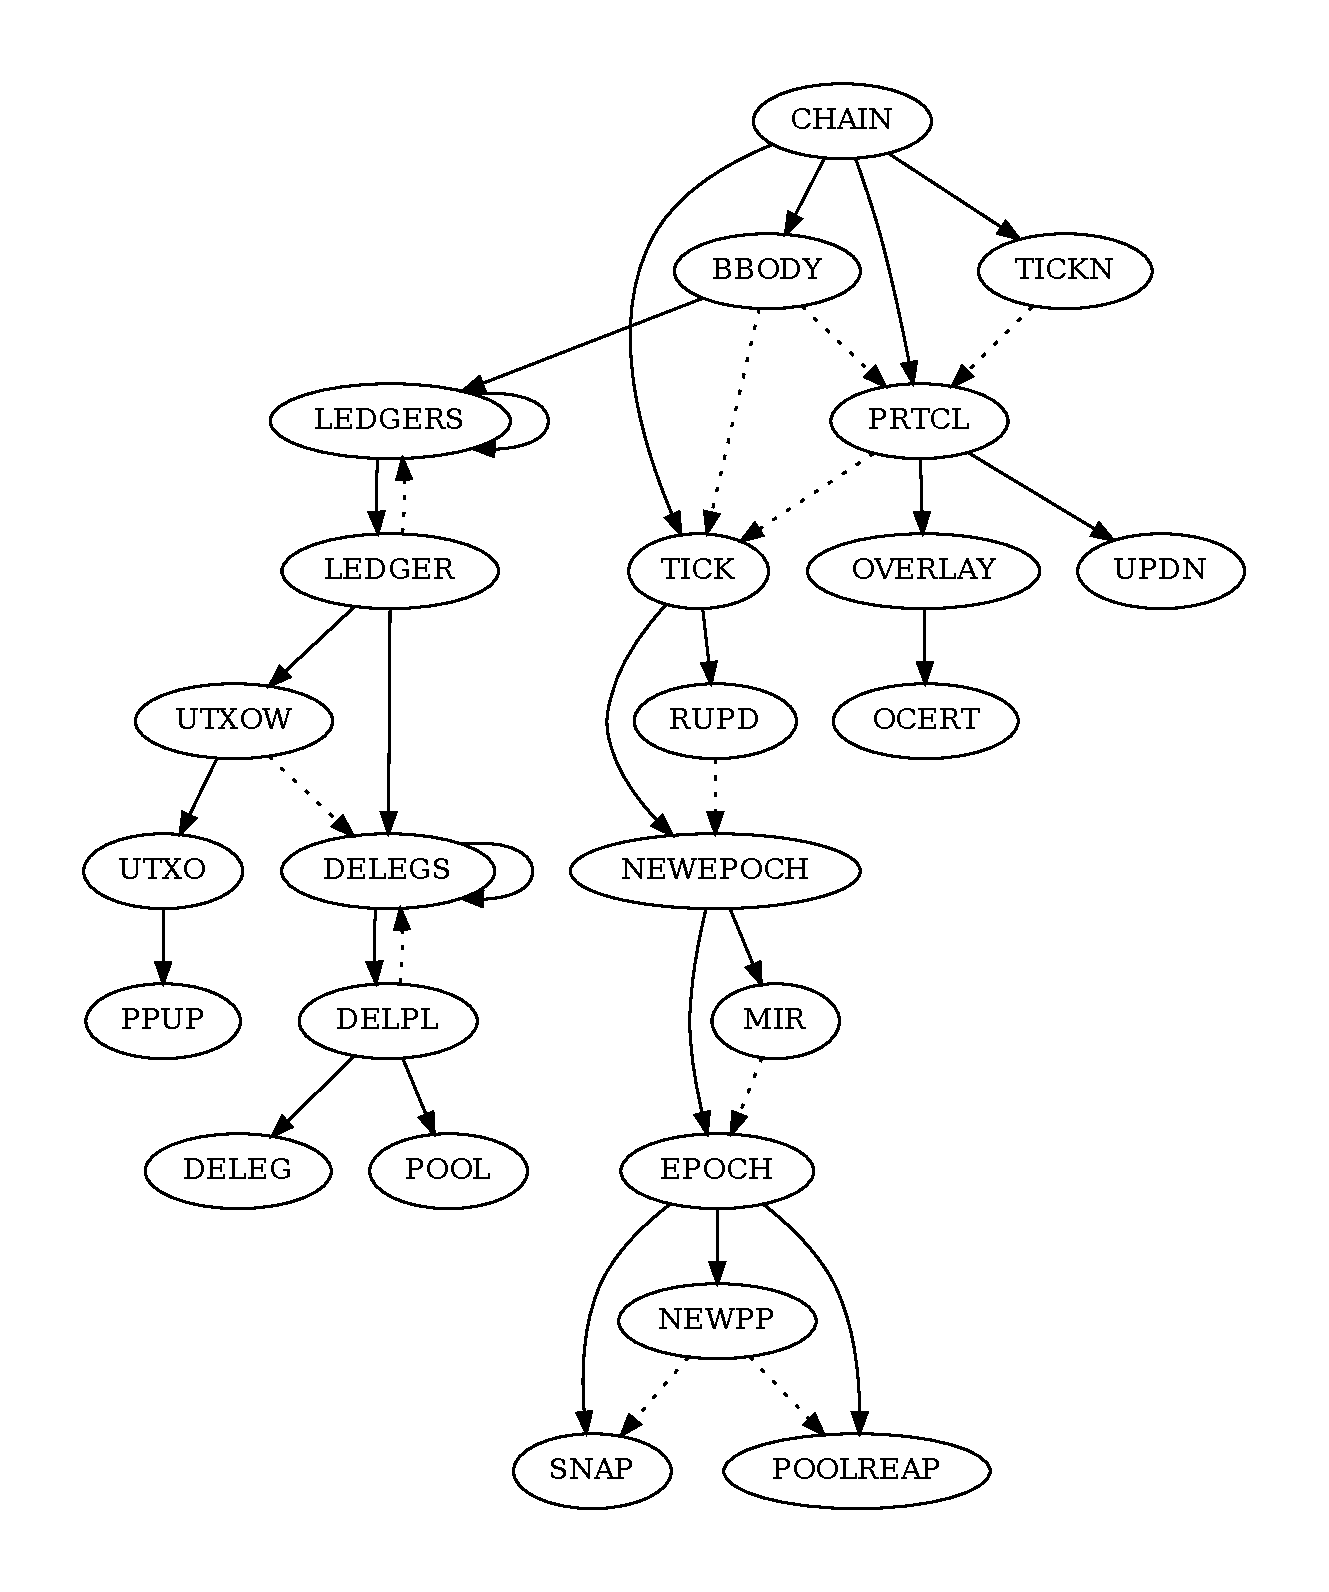
\includegraphics[width=\textwidth]{rules}
  \caption{STS Rules, Sub-Rules and Dependencies}
  \label{fig:sts-rules-dependencies}
\end{figure}

%%% Local Variables:
%%% mode: latex
%%% TeX-master: "ledger-spec"
%%% End:

\newcommand{\Val}{\fun{Val}}
\newcommand{\POV}[1]{\ensuremath{\mathsf{PresOfVal}(\mathsf{#1})}}
\newcommand{\DBE}[2]{\ensuremath{\mathsf{DBE}({#1},~{#2})}}
\newcommand{\DGO}[2]{\ensuremath{\mathsf{DGO}({#1},~{#2})}}
\newcommand{\transtar}[2]{\xlongrightarrow[\textsc{#1}]{#2}\negthickspace^{*}}

\section{Properties}
\label{sec:properties}

This section describes the properties that the ledger should have. The goal is to
to include these properties in the executable specification to enable e.g.
property-based testing or formal verification.

% TODO - the hand proofs of preservation of ada and non-negative deposit
% pot are woefully out of date, mostly due to the removal of decaying deposits.
%
\subsection{Preservation of Value}
\label{sec:preservation-of-value}

As visualized in Figure~\ref{fig:fund-preservation},
the total amount of lovelace in any given chain state
$\var{s}\in\ChainState$ is completely contained within the values of the six
variables:

\begin{tabular}{||l|l|l|l||}\hline\hline

  \textbf{Variable} & \textbf{Name in Figure~\ref{fig:fund-preservation}}
                    & \textbf{Nesting Inside Chain State} & \textbf{Kind} \\ \hline
  utxo & circulation & s.nes.es.ls.utxoSt & Map over Lovelace Values  \\ \hline
  deposits & deposits &  s.nes.es.ls.utxoSt & Lovelace Value ($\Coin$) \\ \hline
  fees & fees &  s.nes.es.ls.utxoSt & Lovelace Value ($\Coin$) \\ \hline
  rewards & reward accounts & s.nes.es.ls.dpstate.dstate  & Lovelace Value ($\Coin$)  \\ \hline
  treasury & treasury &  s.nes.es.acnt  & Lovelace Value ($\Coin$) \\ \hline
  reserves & reserves & s.nes.es.acnt & Map over Lovelace Values \\ \hline
  \hline
\end{tabular}

\noindent
Notice that $\var{deposits}$, $\var{fees}$, $\var{treasury}$, and $\var{reserves}$
are all single lovelace values, while $\var{utxo}$, and $\var{rewards}$ are
maps whose values are lovelace.

We define the \emph{Lovelace Value} of a given chain state as:
\begin{definition}[Lovelace Value]
  \label{def:val}
  \begin{equation*}
    \Val(s~\in~\var{State}) =
        \Val(\var{utxo}) +
            \Val(\var{deposits}) +
            \Val(\var{fees}) +
            \Val(\var{reserves}) +
            \Val(\var{treasury}) +
            \Val(\var{rewards})
  \end{equation*}
  where
  \begin{equation*}
      \Val(x \in \Coin) = x
  \end{equation*}
  \begin{equation*}
      \Val((\wcard\mapsto (y \in \Coin))^{*}) = \sum y
  \end{equation*}
\end{definition}

\noindent
For any state that is used in a given subtransition of $\mathsf{CHAIN}$,
we define $\Val{}$ in an analogous way, setting the value of any variable that is not explicitly
represented in the state to zero.
For example, given $\var{utxoSt}\in\UTxOState$,
\begin{equation*}
  \Val(\var{utxoSt}) =
  \left(\sum_{\wcard\mapsto(\wcard,~v)\in\var{utxo}}v\right) + \var{deposits} + \var{fees}
\end{equation*}

\noindent
The key property that we want to prove is that no semantic transition changes the value that
is captured in the state ($\Val{s}$).
This property is easy to state: intuitively,
the \emph{Lovelace Value}before the transition is the same as the
\emph{Lovelace Value} after that transition.

\begin{theorem}[Preservation of Value]
  \label{thm:chain-pres-of-value}
  For all environments $e$, blocks $b$, and states $s$, $s'$, if
  \begin{equation*}
    e\vdash s\trans{\hyperref[fig:rules:chain]{chain}}{b}s'
  \end{equation*}
  then
  \begin{equation*}
    \Val(s) = \Val(s')
  \end{equation*}
\end{theorem}

\noindent
We will prove the soundness of Theorem~\ref{thm:chain-pres-of-value} via a few lemmas.

\begin{lemma}
  \label{lemma:value-sum-pres-1}
  For any mapping $m:A\mapsto\Coin$ and set $s\in\powerset{A}$,
  \begin{equation*}
    \Val(\var{m}) = \Val(s\subtractdom m) + \Val(s\restrictdom m)
  \end{equation*}
\end{lemma}
\begin{proof}
  easy
\end{proof}

\begin{lemma}
  \label{lemma:value-sum-pres-2}
  For any mappings $m_1, m_2:A\mapsto\Coin$,
  if $\dom{m_1}\cap\dom{m_2}=\emptyset$,
  then
  \begin{equation*}
    \Val(m_1\cup m_2) = \Val(m_1) + \Val(m_2)
  \end{equation*}
\end{lemma}
\begin{proof}
  easy
\end{proof}

\begin{lemma}
  \label{lemma:utxo-pres-of-value}
  For all environments $e$, transactions $t$, and states $s$, $s'$, if
  \begin{equation*}
    e\vdash s\trans{\hyperref[fig:rules:utxo-shelley]{utxo}}{t}s'
  \end{equation*}
  then
  \begin{equation*}
    \Val(s) + w = \Val(s')
  \end{equation*}
  where $w = \fun{wbalance}~(\fun{txwdrls}~{t})$.
\end{lemma}

\begin{proof}
  The proof is essentially unfolding the definition of the predicate
  \begin{equation}
    \label{cons-is-prod}
    \consumed{pp}{utxo}{t} = \produced{pp}{stpools}{t}
  \end{equation}
  and applying a little algebra.
%
If we let:
  \begin{equation*}
    \begin{array}{r@{~=~}l}
      k & \keyRefunds{pp}{stkCreds}{t} \\
      f & \txfee{t} \\
      d & \totalDeposits{pp}{stpools}{(\txcerts{t})} \\
    \end{array}
  \end{equation*}
  then equation~\ref{cons-is-prod} can be rewritten as:
  \begin{equation*}
    \Val(\txins{t} \restrictdom{\var{utxo}}) + w + k = \Val(\outs{t}) + f + d
  \end{equation*}
  where $\outs{}$ is defined in Figure~\ref{fig:functions:utxo} and returns a value of type $\UTxO$.
  Therefore, moving $k$ to the right and adding $\txins{t} \subtractdom{\var{utxo}}$ to each side,
  \begin{equation*}
    \Val(\txins{t} \restrictdom{\var{utxo}}) + \Val(\txins{t} \subtractdom{\var{utxo}}) + w
    = \Val(\outs{t}) + f + d - k + \Val(\txins{t} \subtractdom{\var{utxo}})
  \end{equation*}
  (Though not needed for the proof at hand,
  note that $d-k$ is non-negative since the deposits will always be large enough to cover
  the current obligation. See Theorem~\ref{thm:non-neg-deposits}.)
%
  It then follows that:
  \begin{equation*}
    \begin{array}{r@{~=~}lr}
      \Val(\var{utxo}) + w
    & \Val(\outs{t}) + f + d - k + \Val(\txins{t} \subtractdom{\var{utxo}})
    & \text{(by Lemma~\ref{lemma:value-sum-pres-1})}
    \\
    & \Val((\txins{t} \subtractdom{\var{utxo}})\cup\outs{t}) + (d - k) + f
    & \text{(by Lemma~\ref{lemma:value-sum-pres-2})}
    \end{array}
  \end{equation*}
  Note that in order to apply Lemma~\ref{lemma:value-sum-pres-2} above,
  it must be true that $(\txins{t} \subtractdom{\var{utxo}})$ and $(\outs{t})$
  have disjoint domains, which follows from the uniqueness of the transaction IDs.

  Therefore, by adding the deposits and fees from $s$ to the equality above,
  it follows that $\Val(s) + w = \Val(s')$.
\end{proof}

\begin{lemma}
  \label{lemma:deleg-pres-of-value}
  For all environments $e$, transactions $c$, and states $s$, $s'$, if
  \begin{equation*}
    e\vdash s\trans{\hyperref[fig:delegation-rules]{deleg}}{c}s'
  \end{equation*}
  then
  \begin{equation*}
    \Val(s) = \Val(s')
  \end{equation*}
\end{lemma}

\begin{proof}
  The only variable with value in this transition is \var{rewards}.
  Only two of the rules in $\mathsf{DELEG}$ can change \var{rewards},
  namely $\mathsf{Deleg{-}Reg}$ and $\mathsf{Deleg{-}Dereg}$.
  However, $\mathsf{Deleg{-}Reg}$ only adds a zero value,
  and $\mathsf{Deleg{-}Dereg}$ only removes a zero value.
\end{proof}

\begin{lemma}
  \label{lemma:delegs-pres-of-value}
  For all environments $e$, certificates $\Gamma$, and states $s$, $s'$, if
  \begin{equation*}
    e\vdash s\trans{\hyperref[fig:rules:delegation-sequence]{delegs}}{\Gamma}s'
  \end{equation*}
  then
  \begin{equation*}
    \Val(s) = \Val(s') + w
  \end{equation*}
  where $w = \fun{wbalance}~(\fun{txwdrls}~{t})$,
  and $t$ is the transaction in the environment $e$.
\end{lemma}

\begin{proof}
  The proof is by induction on the length of $\Gamma$.
  Note that the only variable with value in this transition is \var{rewards}.

  \vspace{2ex}
  \noindent
  \emph{In the base case}, we look at the rule $\mathsf{Seq{-}delg{-}base}$.
  Since $\var{wdrls}\subseteq\var{rewards}$, then
  $\var{rewards} = \var{wdrls}\cup\var{(\var{rewards}\setminus\var{wdrls})}$.
%
  Therefore
  \begin{equation*}
    \begin{array}{r@{~=~}lr}
      \Val{(\var{rewards})}
      & \Val{(\var{rewards}\setminus\var{wdrls})} + \Val{(\var{wdrls})}
      & \text{by Lemma~\ref{lemma:value-sum-pres-2}}
      \\
      & \Val{(\var{rewards}\setminus\var{wdrls})} + w
      & \text{by definition}
      \\
      & \Val\left(\var{rewards}\unionoverrideRight\{(w, 0) \mid w \in \dom \var{wdrls}\}\right) + w
    \end{array}
  \end{equation*}
  Therefore $\Val(s) = \Val(s')$.

  \vspace{2ex}
  \noindent
  \emph{In the inductive case}, we look at the rule $\mathsf{Seq{-}delg{-}ind}$.
  In this case, the lemma then follows directly from Lemma~\ref{lemma:deleg-pres-of-value}.
\end{proof}

\begin{lemma}
  \label{lemma:poolreap-pres-of-value}
  For all environments $e$, epoch $\epsilon$, and states $s$, $s'$, if
  \begin{equation*}
    e\vdash s\trans{\hyperref[fig:rules:pool-reap]{poolreap}}{\epsilon}s'
  \end{equation*}
  then
  \begin{equation*}
    \Val(s) = \Val(s')
  \end{equation*}
\end{lemma}

\begin{proof}
  The $\mathsf{POOLREAP}$ value is contained in
  $\var{deposits}$, $\var{treasury}$, and $\var{rewards}$.
  Notice that $\var{unclaimed}$ is added to $\var{treasury}$
  and subtracted from the $\var{deposits}$.
  Moreover, $\var{refunded}$ is subtracted from $\var{deposits}$.
  (Note that $\var{deposits}-(\var{unclaimed}+\var{refunded})$
  is non-negative by Theorem~\ref{thm:non-neg-deposits}.)
  It therefore suffices to show that
  \begin{equation*}
    \begin{array}{r@{~=~}l}
    \Val(\var{rewards}\unionoverridePlus\var{refunds})
    & \Val(\var{rewards}) + \Val(\var{refunds})
    \\
    & \Val(\var{rewards}) + \var{refunded}
    \end{array}
  \end{equation*}
  But this is clear from the definition of $\unionoverridePlus$.
\end{proof}

\begin{lemma}
  \label{lemma:ru-pres-of-value}
  For every $(\Delta t,~\Delta r,~\var{rs},~\Delta f)$ in the range of $\fun{createRUpd}$,
  \begin{equation*}
    \Delta t + \Delta r + \Val(rs) + \Delta f = 0
  \end{equation*}
\end{lemma}

\begin{proof}
  In the definition of $\fun{createRUpd}$ in Figure~\ref{fig:functions:reward-update-creation},
  We see that:
  \begin{equation*}
    \begin{array}{r@{~=~}l}
      \var{rewardPot} & \var{feeSS} + \Delta r \\
      \var{R} & \var{rewardPot} - \Delta t_1 \\
      \Delta t_2 & R - \Val(\var{rs})\\
      \Delta t & \Delta t_1 + \Delta t_2 \\
    \end{array}
  \end{equation*}
  Therefore
  \begin{equation*}
    \begin{array}{r@{~=~}l}
      (\var{feeSS} + \Delta r) & \var{rewardPot} = R + \Delta t_1 = \Delta t_2 + \Val(rs) + \Delta t_1  \\
      0 & (\Delta t_1 + \Delta t_2 ) - \Delta r + \Val(rs)- \var{feeSS} \\
      0 & \Delta t - \Delta r + \Val(rs)- \var{feeSS} \\
    \end{array}
  \end{equation*}
  It then suffices to notice that $\fun{createRUpd}$ returns
  $(\Delta t,-~\Delta r,~\var{rs},~-\var{feeSS})$.
\end{proof}

\noindent

Note that Lemma~\ref{lemma:ru-pres-of-value} is not strictly need for the proof of
Theorem~\ref{thm:chain-pres-of-value}, since the $\mathsf{NEWEPOCH}$ transition
requires that $\Delta t + \Delta r + \Val(rs) + \Delta f = 0$ holds.
It does, however, give us confidence that the $\mathsf{CHAIN}$ transition can proceed.

We are now ready to prove Theorem~\ref{thm:chain-pres-of-value}.

\begin{proof}
  For a given transition $\mathsf{TR}$, let \POV{TR}
  be the statement:

  \begin{tabular}{l}
    for all environments $e$, signals $\sigma$, and states $s$, $s'$,
    $$
    $e\vdash s\trans{tr}{\sigma}s'~\implies~\Val(s) = \Val(s')$.
    $$
  \end{tabular}

  \noindent
  Our goal is to prove \POV{CHAIN}.
  Lemmas~\ref{lemma:utxo-pres-of-value} and \ref{lemma:delegs-pres-of-value} imply \POV{LEDGER},
  since $\mathsf{UTXOW}$ transforms state exactly as $\mathsf{UTXO}$ does.
  \POV{LEDGERS} then follows by straightforward induction on the length of $\Gamma$:
  the base case is trivial;
  and the inductive case follows directly from \POV{LEDGER}.
%
  \POV{SNAP} holds trivially, since it contains no value.
  Similarly, \POV{NEWPP} holds since $\var{diff}$ is added to $\var{reserves}$
  and subtracted from $\var{deposits}$.
  Therefore \POV{EPOCH} holds by Lemma~\ref{lemma:poolreap-pres-of-value}.
  \POV{MIR} holds since
  $\Val{i_{rwd}'}=\var{tot}$ in Figure~\ref{fig:rules:mir}.
  Morover, \POV{NEWEPOCH} holds in the presence of $\fun{applyRUpd}$
  since the transition requires $\Delta t + \Delta r + \Val(rs) + \Delta f = 0$.
  \POV{CHAIN} easily follows from this.
\end{proof}

\subsection{Non-negative Deposit Pot}  % TODO - this section is out of date due to no decaying deposits
\label{sec:non-negative-deposit-pot}

The \emph{deposit pot} (the variable $\var{deposits}$ in the UTxO State)
represents the amount of \emph{lovelace} that is set aside by the system as a whole for refunding deposits.
Deposits are added to this pot, which then decays exponentially over time,
and is also depleted by any refunded deposits.
At an epoch boundary, the decayed parts of any deposits (including, possibly, deposits for any transactions that will complete in future epochs)
will be distributed as additional \emph{rewards}, as described in~\cite{delegation_design}.
Since $\var{deposits}$ is only used to record the value of future refunds or rewards whose costs have
already been incurred, both it and any reward value will always be non-negative.
Note that there are two types of deposits which are recorded in the same pot: those for stake keys; and those for stake pools.
Stake keys are deregistered in the slot in which the deregistration certificates
is processed. Stake pools, however, are staged for retirement on epoch boundaries.
%
The following theorem ensures that the deposit pot is properly maintained
and will always be large enough to meet all of its obligations.


\begin{figure}[h!]
  \begin{tabular}{||l|l|l|l||}\hline\hline

    \textbf{Variable} & \textbf{Value}
                      & \textbf{Nesting Inside Chain State} & \textbf{Kind} \\ \hline
    deposits & 0 &  s.nes.es.ls.utxoSt & $\Coin$ \\ \hline
    stkCreds & $\emptyset$ & s.nes.es.ls.dpstate.dstate.stkCreds
             & $\StakeCreds$ ($\Credential\mapsto\Slot$)  \\ \hline
    stpools & $\emptyset$ & s.nes.es.ls.dpstate.pstate.stpools
            & $\StakePools$ ($\KeyHash\mapsto\Slot$)  \\ \hline
  \end{tabular}
  \caption{Initial Chain State}
  \end{figure}

\begin{theorem}[Non-negative Deposit Pot]
  \label{thm:non-neg-deposits}
  Let $n\in\N$ and $c_0\in\ChainState$ be a chain state in which $\var{deposits} ~=~0$, $\var{stkCreds}~=~\emptyset$ and $\var{stPools}~=~\emptyset$, as shown above:
%  \\~\\
  If
  \begin{equation*}
    s_0\vdash c_0\trans{\hyperref[fig:rules:chain]{chain}}{b_0}c_1,~~
    s_1\vdash c_1\trans{\hyperref[fig:rules:chain]{chain}}{b_1}c_2,~~
    \ldots,~~
    s_n\vdash c_n\trans{\hyperref[fig:rules:chain]{chain}}{b_n}c_{n+1},~~n \ge 0
  \end{equation*}
  is a sequence of valid $\mathsf{CHAIN}$ transitions,
  then $\forall i, 0 \le i \le n, \var{deposits} ~(c_{n+1}) \ge 0$.
\end{theorem}

\begin{proof}

  We will prove a slightly stronger condition, namely that some stronger invariants hold
  most of the time, and that when they do fail to hold, then $\var{deposits}$ is still non-negative.
  These stronger invariants will require a few additional definitions.
%
  Given a slot $s$, let $\ell(s)$ be the first slot of the epoch that $s$ occurs in,
  that is $\ell = \fun{firstSlot}\circ\fun{epoch}$.
  Given a mapping $m\in\mathsf{T}\to\Slot$ and a slot $s\in\Slot$,
  let $\fun{sep}$ be the function that separates $m$ into two maps,
  those whose value is strictly less than $s$ and those whose value is at least $s$.
  So,
  \begin{equation*}
    \fun{sep}~m~s = \forall x\mapsto t~\in~m,~~
    \left(\{x\mapsto t~\mid~t<s\},~\{x\mapsto t~\mid~t\geq s\}\right)
  \end{equation*}


  \noindent
  If we assume that the \emph{protocol parameters}, $pp$, are fixed\footnote{Note that the
    protocol parameters can only change in the $\mathsf{NEWPP}$ transition.}, then we can provide convenience functions
  $R_c$ and $R_p$ for the \emph{stake credential} and \emph{stake pool} refunds, respectively:
  \begin{equation*}
    \begin{array}{r@{~=~}l}
      R_c~s_0~s_1 & \refund{d_{val}}{d_{min}}{\lambda_d}{s_1-s_0} \\
      R_p~s_0~s_1 & \refund{p_{val}}{p_{min}}{\lambda_p}{s_1-s_0} \\
    \end{array}
  \end{equation*}
  where $d_{val}$, $d_{min}$, $\lambda_d$, $p_{val}$, $p_{min}$, $\lambda_p$
  are the protocol parameter values from $pp$, and $\fun{refund}$ is defined in
  Figure~\ref{fig:functions:deposits-refunds}.
  We let \DBE{c}{s} (``Deposits (precisely) Big Enough"), be the following property:
  \begin{equation}\tag{DBE}\label{DBE}
    \var{deposits}
    = \left(\sum_{\wcard\mapsto t\in C_{old}}R_c~t~\ell(s)\right)
    + |C_{new}|\cdot d_{val}
    + \left(\sum_{\wcard\mapsto t\in P_{old}}R_p~t~\ell(s)\right)
    + |P_{new}|\cdot p_{val}
  \end{equation}
  where
  \begin{equation*}
    \begin{array}{r@{~=~}l}
      C_{old},~C_{new} & \fun{sep}~\var{stkCreds}~{\ell(s)} \\
      P_{old},~P_{new} & \fun{sep}~\var{stpools}~{\ell(s)},
    \end{array}
  \end{equation*}
  for some slot, $s$, where $\var{pp}$, $\var{stkCreds}$, $\var{stpools}$ are in the corresponding chain state, $c$.
%
  In other words, \DBE{c}{s} asserts that the deposit pot is equal to the
  sum of the deposit refunds that were available at the previous epoch boundary,
  plus the sum of the initial deposit values for all the deposits from the current epoch.

  Notice that for a chain state $c$ and slot $s$, if the range of
  $\var{stkCreds}$ and $\var{stpools}$ contains only slots from the previous epoch,
  then \DBE{c}{s} is equivalent to
  \begin{equation}\tag{DEO}\label{DEO}
    \var{deposits} = \obligation{pp}{stkCreds}{stpools}{\ell(s)}
  \end{equation}
  where $\fun{obligation}$ is defined in Figure~\ref{fig:funcs:epoch-helper-rewards}.
%
  It is generally true that \DBE{c'}{s_i} holds after each subtransition of
  $s_i\vdash c_i\trans{\hyperref[fig:rules:chain]{chain}}{b_i}c_{i+1}$.
  However, this invariant can fail to hold after the
  $\hyperref[fig:delegation-transitions]{\mathsf{DELEG}}$ transition,
  since this transition can add and remove stake credentials, and can also add stake pools,
  but the deposit pot is not adjusted accordingly
  until the next subtransiton of $\hyperref[fig:rules:ledger]{\mathsf{LEDGER}}$,
  namely $\hyperref[fig:rules:utxo-shelley]{\mathsf{UTXO}}$.
%
  The invariant can also fail to hold if the slot increases while the chain state remains the same.
  That is, if \DBE{c_{i+1}}{s_i} holds, then \DBE{c_{i+1}}{s_{i+1}} can fail to hold if
  $\epoch{s_i} < \epoch{s_{i+1}}$, since the value of the deposit
  in the left hand side of equation~\ref{DBE} remains the same, but the
  refunded values become smaller\footnote{Note that if $\epoch{s_i} = \epoch{s_{i+1}}$, then \DBE{c_{i+1}}{s_{i+1}} is trivially true.}.
  Therefore, in this situation we can consider the slightly weaker constraint:
  \begin{equation}\tag{DGO}\label{DGTO}
    \var{deposits} \geq \obligation{pp}{stkCreds}{stpools}{\ell(s)}
  \end{equation}
  The difference between the left and right hand sides of the inequality
  corresponds to the lovelace value in $c_{i+1}$ that decays between $s_i$ and $s_{i+1}$.

  There are four sub-transitions where $\var{deposits}$ is changed:
  $\mathsf{SNAP}$ (Figure~\ref{fig:rules:snapshot}),
  $\mathsf{POOLREAP}$ (Figure~\ref{fig:rules:pool-reap}),
  $\mathsf{NEWPP}$ (Figure~\ref{fig:rules:new-proto-param}),
  $\mathsf{UTXO}$ (Figure~\ref{fig:rules:utxo-shelley}).
  This ordering is also the order in which $\var{deposits}$ is changed.
  Of these sub-transitions, only $\mathsf{UTXO}$ actually changes the value of $\var{deposits}$
  when $s_i$ is in the same epoch as $s_i$.
  (We say that $s_i$ \emph{crosses the epoch boundary} if the precondition of
  Rule~\ref{eq:new-epoch} in Figure~\ref{fig:rules:new-epoch} is met,
  namely if $\epoch{s_i} \ge e_\ell+1$.)
%
  The proof then proceeds by induction on $n$, showing the following:
  \begin{itemize}
    \item
      Let $c$ be the chain state after the $\mathsf{SNAP}$ transition
      in $s_i\vdash c_i\trans{\hyperref[fig:rules:chain]{chain}}{b_i}c_{i+1}$.
      If \DGO{c_i}{s_i}, then \DBE{c}{s_i} holds.
    \item $\mathsf{POOLREAP}$ preserves \ref{DBE}.
    \item $\mathsf{NEWPP}$ preserves \ref{DBE}.
    \item The property for $\mathsf{UTXO}$ requires a bit of explanation.
      Let $\var{nes}\in\NewEpochState$ be the new epoch state in $c_i$.
      Note that the property \ref{DBE} makes sense for values of $\NewEpochState$
      since it contains all the relevant variables.
      Similarly, \ref{DBE} also makes sense for values of $\UTxOState\times\PParams$.
      Let
      $$
        {\begin{array}{c}
           \var{gkeys} \\
         \end{array}}
        \vdash\var{nes}\trans{\hyperref[fig:rules:tick]{tick}}{\var{bh}}\var{nes'}
      $$
      be the first sub-transition of
      $s_i\vdash c_i\trans{\hyperref[fig:rules:chain]{chain}}{b_i}c_{i+1}$.
      If \DBE{\var{nes'}}{s_i} holds, then \DBE{(us', pp)}{s_i} holds for every transaction
      $tx$ in $b_i$, where:
      $$
      \var{env}\vdash \var{us} \trans{\hyperref[fig:rules:utxow-shelley]{utxo}}{tx} \var{us'},
      $$
      is a sub-transition of
      $s_i\vdash c_i\trans{\hyperref[fig:rules:chain]{chain}}{b_i}c_{i+1}$,
      and $\var{pp}$ is the protocol parameters in $\var{nes'}$.
  \end{itemize}

  \noindent
  Case $\hyperref[fig:rules:snapshot]{\mathsf{SNAP}}$.
  We must show that
  if $c$ is the chain state after the $\mathsf{SNAP}$ transition
  in $s_i\vdash c_i\trans{\hyperref[fig:rules:chain]{chain}}{b_i}c_{i+1}$,
  and \DGO{c_i}{s_i} holds, then so does \DBE{c}{s_i}.
%
  We can assume that $s_i$ crosses the epoch boundary,
  since otherwise the $\mathsf{SNAP}$ transition will not occur.
  Since the $\mathsf{SNAP}$ transition only happens within the $\mathsf{TICK}$ transition
  on the epoch boundary, it follows that
  $c_i$ does not contain any stake credentials or pools from the current epoch,
  and so \ref{DBE} will be equivalent to \ref{DEO} (the current epoch is $\epoch{s_i}$).
  However, \DBE{c}{s_i} holds trivially, since it is determined from the $\fun{obligation}$ value.
  \\~\\
  Case $\hyperref[fig:rules:pool-reap]{\mathsf{POOLREAP}}$.
  We must show that \ref{DBE} is preserved.
%
  We again assume that $s_i$ crosses the epoch boundary.
  The $\mathsf{POOLREAP}$ transition does the following:
  \begin{enumerate}
    \item leaves $\var{stkCreds}$ unchanged,
    \item removes $\var{retired}$ from $\var{stpools}$,
    \item subtracts $\var{unclaimed}+\var{refunded}$ from $\var{deposits}$.
  \end{enumerate}
%
  Notice that the domain of the $\var{pr}$ is $\var{retired}$,
  and similarly the domain of the $\var{rewardAcnts}$ is also $\var{retired}$
  since the domains of $\var{stpools}$ and $\var{poolParams}$ are the same.
  Therefore $\var{retired}$ is the disjoint union of
  $\dom({\var{refunds}})$ and $\dom({\var{mRefunds}})$, so that
  \begin{equation*}
    \begin{array}{r@{~=~}l}
      \var{unclaimed}+\var{refunded}
      &
      \left(
        \sum\limits_{\wcard\mapsto t\in\var{refunds}}R_p~t~\ell(s)
      \right)+
      \left(
        \sum\limits_{\wcard\mapsto t\in\var{mRefunds}}R_p~t~\ell(s)
      \right)
      \\
      &
      \sum\limits_{\wcard\mapsto t\in\var{rewardAcnts'}}R_p~t~\ell(s)
      \\
      &
      \left(
        \sum\limits_{\wcard\mapsto t\in\var{stpools}}R_p~t~\ell(s)
      \right)-
      \left(
        \sum\limits_{\wcard\mapsto t\in\var{retired}\subtractdom\var{stpools}}R_p~t~\ell(s)
      \right)
    \end{array}
  \end{equation*}
  Therefore, it follows that if \ref{DEO} holds before $\mathsf{POOLREAP}$, then it also holds afterwards.
  \\~\\
  Case $\hyperref[fig:rules:new-proto-param]{\mathsf{NEWPP}}$.
  We must show that \ref{DBE} is preserved.
%
  We again assume that $s_i$ crosses the epoch boundary.
  In this transition $\var{pp}$ can change, but $\var{stkCreds}$, $\var{stpools}$,
  and $\var{deposits}$ do not change.
  As in the $\mathsf{SNAP}$ case, \DBE{c}{s_i} holds trivially,
  since it is set to the value that is determined by $\fun{obligation}$.
  \\~\\
  Case $\hyperref[fig:rules:utxo-shelley]{\mathsf{UTXO}}$.
  We assume that \DBE{\var{nes'}}{s_i} holds, where $\var{nes'}$
  is the new epoch state after the $\mathsf{TICK}$ transition.
  We must show that \ref{DBE} is preserved after each $\mathsf{UTXO}$ transition.
%
  The $\mathsf{DELEGS}$ transition can result in values being
  added to or deleted from $\var{stkCreds}$, and added to $\var{stpools}$.
  Let $A_s$ be the added stake credentials, $D_s$ be the deleted credentials, and
  $A_p$ be the added stake pools, where $\var{stkCreds}'$ is the stake credential mapping
   $\var{stpools}'$ is the stake pools, and $\var{deposits}'$ is the deposit pot  after $\mathsf{DELEGS}$.
  We have that
  \begin{equation*}
    \begin{array}{rcl}
      \var{D_s} & \subseteq & \var{\var{stkCreds}\cup\var{A_s}} \\
      \var{stkCreds}' & = & (\var{stkCreds}\cup\var{A_s})\setminus\var{D_s} \\
      \var{stpools}' & = & \var{stpools}\cup\var{A_p} \\
    \end{array}
  \end{equation*}
  The slots in the range of $A_s$ will all be equal to $s_i$,
  but the slots in the range of $D_s$
may either be from the current epoch or an earlier one, so we split them using $\fun{sep}$:
  \begin{equation*}
    (\var{D_{s\_old}},~\var{D_{s\_new}}) = \fun{sep}~\var{D_s}~\ell(s_i)
  \end{equation*}
  We must then show that
  \begin{equation*}
    \var{deposits}' = \var{deposits}
    + |A_s|\cdot d_{val}
    + |P_c|\cdot p_{val}
    - |D_{s\_new}|\cdot d_{val}
    - \left(\sum_{\wcard\mapsto t\in D_{s\_old}}R_c~t~\ell(s_i)\right)
  \end{equation*}
  Looking at the $\mathsf{UTXO}$ transition in Figure~\ref{fig:rules:utxo-shelley},
  \begin{equation*}
    \var{deposits}' = \var{deposits} + \totalDeposits{pp}{stpools}{(\txcerts{tx})}
    - (\var{refunded} + \var{decayed})
  \end{equation*}
  The function $\fun{totalDeposits}$ is defined in Figure~\ref{fig:functions:deposits-refunds}
  and it is clear that here it is equal to
  $$|A_s|\cdot d_{val} + |P_c|\cdot p_{val.}$$
  Recall that
  \begin{equation*}
    \begin{array}{r@{~=~}l}
      \var{refunded} & \keyRefunds{pp}{stkCreds}~{tx} \\
      \var{decayed} & \decayedTx{pp}{stkCreds}~{tx}
    \end{array}
  \end{equation*}
  where $\fun{keyRefunds}$ is defined in Figure~\ref{fig:functions:deposits-refunds}.
  This iterates $\fun{keyRefund}$ from the same figure,
  which in turn just looks up the creation slot for a transaction and returns $R_c$.
  The function to calculate the value of decayed deposits, $\fun{decayedTx}$, is defined in Figure~\ref{fig:functions:deposits-decay}.
  This iterates $\fun{decayedKey}$ from the same figure.
  Therefore, to show that
  \begin{equation}\label{deleted-is-refunds-plus-decayed}
    |D_{s\_new}|\cdot d_{val} + \sum_{\wcard\mapsto t\in D_{s\_old}}R_c~t~\ell(s_i)
    = \var{refunded} + \var{decayed},
  \end{equation}
  and thus complete the proof for the $\mathsf{UTXO}$ case,
  it suffices to show that for a given $\var{c}\mapsto s\in D_s$,
  the $R_c$ value plus the $\fun{decayedKey}$ value that is associated with the stake
  credential $c$ is equal to $d_{val}$ if $\epoch(s)=\epoch(s_i)$, and is otherwise equal to $R_c~s~\ell(s_i)$.
  Looking at the definition of $\fun{decayedKey}$, observe that if $\epoch(s)=\epoch(s_i)$
  then $\var{start}=\var{created}$ and so the decayed value is $(R_c~s~s)-(R_c~s~s_i)$.
  However, $R_c~s~s = d_{val}$, so the refund plus the decayed value is
  $d_{val}-(R_c~s~s_i)+(R_c~s~s_i)=d_{val}$.
  Otherwise, if $s$ is from a previous epoch, then $\var{start}=\ell(s_i)$, and so
  the decayed value is $(R_c~s~\ell(s_i))-(R_c~s~s_i)$.
  The refund plus the decayed value is thus
  $(R_c~s~\ell(s_i))-(R_c~s~s_i)+(R_c~s~s_i)=(R_c~s~\ell(s_i))$.
  Therefore, equation~\ref{deleted-is-refunds-plus-decayed} holds, and
  consequently so also does \DBE{c'}{s_i}.

\end{proof}



\subsection{Header-Only Validation}
\label{sec:header-only-validation}
The header-only validation properties of the Shelley Ledger are the analogs
of those from Section 8.1 of \cite{byron_chain_spec}.

In any given chain state, the consensus layer needs to be able to validate the
block headers without having to download the block bodies.
Property~\ref{prop:header-only-validation} states that if an extension of a
chain that spans less than $\StabilityWindow$ slots is valid, then validating the
headers of that extension is also valid. This property is useful for its
converse: if the header validation check for a sequence of headers does not
pass, then we know that the block validation that corresponds to those headers
will not pass either.

First we define the header-only version of the $\mathsf{CHAIN}$ transition,
which we call $\mathsf{CHAINHEAD}$.
It is very similar to $\mathsf{CHAIN}$, the differences being:
\begin{itemize}
  \item The $\mathsf{CHAINHEAD}$ signal is not a block, but a block header ($\BHeader$).
  \item $\mathsf{CHAINHEAD}$ does not call $\mathsf{BBODY}$.
  \item $\mathsf{CHAINHEAD}$ does not call $\mathsf{TICK}$, but instead
    calls the similar $\mathsf{TICKF}$, which differs by
    not calling the reward update transition $\mathsf{RUPD}$.
  \item $\mathsf{CHAINHEAD}$ does not store the new epoch state $\var{nes}$ in
    its state, but rather contains it in the environment.
    We will conveniently \textbf{abuse the tuple notation} and write
    $(nes, \tilde{s}) = s$
    for splitting the chain state into the new epoch state and the remaiing fields.
\end{itemize}

\begin{figure}[ht]
  \begin{equation}\label{eq:tickf}
    \inference[TickForecast]
    {
      {
        \vdash
        \var{nes}
        \trans{\hyperref[fig:rules:new-epoch]{newepoch}}{\epoch{slot}}
        \var{nes}'
      }
      \\~\\
      (\var{e_\ell'},~\var{b_{prev}'},~\var{b_{cur}'},~\var{es'},~\var{ru'},~\var{pd'})
      \leteq\var{nes'}
      \\
      \var{es''}\leteq\fun{adoptGenesisDelegs}~\var{es'}~\var{slot}
      \\
      \var{forecast}\leteq
      (\var{e_\ell'},~\var{b_{prev}'},~\var{b_{cur}'},~\var{es''},~\var{ru'},~\var{pd'})
      \\~\\
    }
    {
      \vdash\var{nes}\trans{tickf}{\var{slot}}\varUpdate{\var{forecast}}
    }
  \end{equation}
  \caption{Tick Forecast rules}
  \label{fig:rules:tickf}
\end{figure}

\clearpage

\begin{figure}[ht]
  \begin{equation}\label{eq:chain-head}
    \inference[ChainHead]
    {
      \var{bhb} \leteq \bhbody{bh}
      &
      \var{s} \leteq \bslot{bhb}
      \\~\\
      \fun{prtlSeqChecks}~\var{lab}~\var{bh}
      \\~\\
      {
        \vdash\var{nes}\trans{\hyperref[fig:rules:tickf]{tickf}}{\var{s}}\var{forecast}
      } \\~\\
      (\var{e_1},~\wcard,~\wcard,~\wcard,~\wcard,~\wcard)
        \leteq\var{nes} \\
      (\var{e_2},~\wcard,~\wcard,~\var{es},~\wcard,~\wcard,~\var{pd})
        \leteq\var{forecast} \\
        (\var{acnt},~\wcard,\var{ls},~\wcard,~\var{pp})\leteq\var{es}\\
        ( \wcard,
          ( (\wcard,~\wcard,~\wcard,~\wcard,~\var{genDelegs},~\wcard),~
          (\wcard,~\wcard,~\wcard)))\leteq\var{ls}\\
          \var{ne} \leteq  \var{e_1} \neq \var{e_2}\\
          \eta_{ph} \leteq \prevHashToNonce{(\lastAppliedHash{lab})} \\~\\
      \fun{chainChecks}~
        \MaxMajorPV~(\fun{maxHeaderSize}~\var{pp},~\fun{maxBlockSize}~\var{pp},~\fun{pv}~\var{pp})~
        \var{bh}\\~\\
      {
        {\begin{array}{c}
        \var{pp} \\
        \eta_c \\
        \eta_\var{ph} \\
        \end{array}}
        \vdash
        {\left(\begin{array}{c}
        \eta_0 \\
        \eta_h \\
        \end{array}\right)}
        \trans{\hyperref[fig:rules:tick-nonce]{tickn}}{\var{ne}}
        {\left(\begin{array}{c}
        \eta_0' \\
        \eta_h' \\
        \end{array}\right)}
      }\\~\\~\\
      {
        {\begin{array}{c}
            (\fun{d}~\var{pp}) \\
            \var{pd} \\
            \var{genDelegs} \\
            \eta_0' \\
         \end{array}}
        \vdash
        {\left(\begin{array}{c}
              \var{cs} \\
              \eta_v \\
              \eta_c \\
        \end{array}\right)}
        \trans{\hyperref[fig:rules:prtcl]{prtcl}}{\var{bh}}
        {\left(\begin{array}{c}
              \var{cs'} \\
              \eta_v' \\
              \eta_c' \\
        \end{array}\right)}
      } \\~\\~\\
      \var{lab'}\leteq (\bblockno{bhb},~\var{s},~\bhash{bh} ) \\
    }
    {
      \var{nes}
      \vdash
      {\left(\begin{array}{c}
            \var{cs} \\
            \eta_0 \\
            \eta_v \\
            \eta_c \\
            \eta_h \\
            \var{lab} \\
      \end{array}\right)}
      \trans{chainhead}{\var{bh}}
      {\left(\begin{array}{c}
            \varUpdate{\var{cs}'} \\
            \varUpdate{\eta_0'} \\
            \varUpdate{\eta_v'} \\
            \varUpdate{\eta_c'} \\
            \varUpdate{\eta_h'} \\
            \varUpdate{\var{lab}'} \\
      \end{array}\right)}
    }
  \end{equation}
  \caption{Chain-Head rules}
  \label{fig:rules:chainhead}
\end{figure}

\begin{property}[Header only validation]\label{prop:header-only-validation}
  For all states $s$ with slot number $t$\footnote{i.e. the
    component $\var{s_\ell}$ of the last applied block of $s$ equals $t$},
    and chain extensions $E$ with corresponding headers $H$ such that:
  %
  $$
  0 \leq t_E - t  \leq \StabilityWindow
  $$
  %
  we have:
  %
  $$
  \vdash s \transtar{\hyperref[fig:rules:chain]{chain}}{E} s'
  \implies
  \var{nes} \vdash \tilde{s} \transtar{\hyperref[fig:rules:chainhead]{chainhead}}{H} s''
  $$
  where $s=(\var{nes},~\tilde{s})$,
  $t_E$ is the maximum slot number appearing in the blocks contained in
  $E$, and $H$ is obtained from $E$ by applying $\fun{bheader}$ to each block in $E$.
\end{property}

\begin{property}[Body only validation]\label{prop:body-only-validation}
  For all states $s$ with slot number $t$, and chain
  extensions $E = [b_0, \ldots, b_n]$ with corresponding headers $H$ such that:
  $$
  0 \leq t_E - t  \leq \StabilityWindow
  $$
  we have that for all $i \in [1, n]$:
  $$
  \var{nes} \vdash \tilde{s} \transtar{\hyperref[fig:rules:chainhead]{chainhead}}{H} s_{h}
  \wedge
  \vdash (\var{nes},~\tilde{s}) \transtar{\hyperref[fig:rules:chain]{chain}}{[b_0 \ldots b_{i-1}]} s_{i-1}
  \implies
  \var{nes'} \vdash \tilde{s}_{i-1}\trans{\hyperref[fig:rules:chainhead]{chainhead}}{h_i} s'_{h}
  $$
  where $s_{i-1}=(\var{nes'},~\tilde{s}_{i-1})$,
  $t_E$ is the maximum slot number appearing in the blocks contained in $E$.
\end{property}

Property~\ref{prop:body-only-validation} states that if we validate a sequence
of headers, we can validate their bodies independently and be sure that the
blocks will pass the chain validation rule. To see this, given an environment
$e$ and initial state $s$, assume that a sequence of headers
$H = [h_0, \ldots, h_n]$ corresponding to blocks in $E = [b_0, \ldots, b_n]$ is
valid according to the $\mathsf{chainhead}$ transition system:
%
$$
\var{nes} \vdash \tilde{s} \transtar{\hyperref[fig:rules:chainhead]{chainhead}}{H} \tilde{s'}
$$
%
Assume the bodies of $E$ are valid
according to the $\mathsf{bbody}$ rules, but $E$ is not valid according to
the $\mathsf{chain}$ rule. Assume that there is a $b_j \in E$ such that it is
\textbf{the first block} such that does not pass the $\mathsf{chain}$
validation. Then:
%
$$
\vdash (\var{nes},~\tilde{s}) \transtar{\hyperref[fig:rules:chain]{chain}}{[b_0, \ldots b_{j-1}]} s_j
$$
But by Property~\ref{prop:body-only-validation} we know that
%
$$
\var{nes}_j \vdash \tilde{s}_j \trans{\hyperref[fig:rules:chainhead]{chainhead}}{h_j} \tilde{s}_{j+1}
$$
which means that block $b_j$ has valid headers, and this in turn means that the
validation of $b_j$ according to the chain rules must have failed because it
contained an invalid block body. But this contradicts our assumption that the
block bodies were valid.

\begin{property}[Existence of roll back function]\label{prop:roll-back-funk}
  There exists a function $\fun{f}$ such that for all chains
  $$C = C_0 ; b; C_1$$
  we have that if for all alternative chains $C'_1$, $\size{C'_1} \leq \frac{\StabilityWindow}{2}$, with
  corresponding headers $H'_1$
  $$
  \vdash s_0 \transtar{\hyperref[fig:rules:chain]{chain}}{C_0;b} s_1 \transtar{\hyperref[fig:rules:chain]{chain}}{C_1} s_2
  \wedge
  \vdash s_1 \transtar{\hyperref[fig:rules:chain]{chain}}{C_1'} s'_1
  \implies
  \var{nes} \vdash \tilde{s} \transtar{\hyperref[fig:rules:chainhead]{chainhead}}{H'_1} s_h
  $$
\end{property}
where $\fun{f}~(\bheader{b})~s_2=(\var{nes},~\tilde{s})$.

Property~\ref{prop:roll-back-funk} expresses the fact the there is a function
that allow us to recover the header-only state by rolling back at most $k$
blocks, and use this state to validate the headers of an alternate chain. Note
that this property is not inherent to the $\mathsf{chain}$ rules and can be
trivially satisfied by any function that keeps track of the history of the
intermediate chain states up to $k$ blocks back. This property is stated here
so that it can be used as a reference for the tests in the consensus layer,
which uses the rules presented in this document.


\subsection{Validity of a Ledger State}
\label{sec:valid-ledg-state}

Many properties only make sense when applied to a valid ledger state. In
informal terms, a valid ledger state $l$ can only be reached when starting from
an initial state $l_{0}$ (ledger in the genesis state) and only executing LEDGER
state transition rules as specified in Section~\ref{sec:ledger-trans} which
changes either the UTxO or the delegation state.

\begin{figure}[ht]
  \centering
  \begin{align*}
    \genesisId & \in & \TxId \\
    \genesisTxOut & \in & \TxOut \\
    \genesisUTxO & \coloneqq & (\genesisId, 0) \mapsto \genesisTxOut
    \\
    \ledgerState & \in & \left(
                         \begin{array}{c}
                           \UTxOState \\
                           \DPState
                         \end{array}
    \right)\\
               && \\
    \fun{getUTxO} & \in & \UTxOState \to \UTxO \\
    \fun{getUTxO} & \coloneqq & (\var{utxo}, \wcard, \wcard, \wcard) \mapsto \var{utxo}
  \end{align*}
  \caption{Definitions and Functions for Valid Ledger State}
  \label{fig:valid-ledger}
\end{figure}

In Figure~\ref{fig:valid-ledger} \genesisId{} marks the transaction identifier
of the initial coin distribution, where \genesisTxOut{} represents the initial
UTxO. It should be noted that no corresponding inputs exists, i.e., the
transaction inputs are the empty set for the initial transaction. The function
\fun{getUTxO} extracts the UTxO from a UTxO state.

\begin{definition}[\textbf{Valid Ledger State}]
  \begin{multline*}
    \forall l_{0},\ldots,l_{n} \in \LState, lenv_{0},\ldots,lenv_{n} \in \LEnv,
    l_{0} = \left(
      \begin{array}{c}
        \genesisUTxOState \\
        \left(
        \begin{array}{c}
          \emptyset\\
          \emptyset
        \end{array}
        \right)
      \end{array}
    \right)  \\
    \implies \forall 0 < i \leq n, (\exists tx_{i} \in \Tx,
    lenv_{i-1}\vdash l_{i-1} \trans{ledger}{tx_{i}} l_{i}) \implies
    \applyFun{validLedgerState} l_{n}
  \end{multline*}
  \label{def:valid-ledger-state}
\end{definition}

Definition~\ref{def:valid-ledger-state} defines a valid ledger state reachable
from the genesis state via valid LEDGER STS transitions. This gives a
constructive rule how to reach a valid ledger state.

\subsection{Ledger Properties}
\label{sec:ledger-properties}

The following properties state the desired features of updating a valid ledger
state.

\begin{property}[\textbf{Preserve Balance}]
  \begin{multline*}
    \forall \var{l}, \var{l'} \in \LState: \applyFun{validLedgerstate}{l},
    l=(u,\wcard,\wcard,\wcard), l' = (u',\wcard,\wcard,\wcard)\\
    \implies \forall \var{tx} \in \Tx, lenv \in\LEnv, lenv \vdash\var{u} \trans{utxow}{tx} \var{u'} \\
    \implies \applyFun{destroyed}{pc~utxo~stkCreds~rewards~tx} =
    \applyFun{created}{pc~stPools~tx}
  \end{multline*}
  \label{prop:ledger-properties-1}
\end{property}

Property~\ref{prop:ledger-properties-1} states that for each valid ledger $l$,
if a transaction $tx$ is added to the ledger via the state transition rule UTXOW
to the new ledger state $l'$, the balance of the UTxOs in $l$ equals the balance
of the UTxOs in $l'$ in the sense that the amount of created value in $l'$
equals the amount of destroyed value in $l$. This means that the total amount of
value is left unchanged by a transaction.

\begin{property}[\textbf{Preserve Balance Restricted to TxIns in Balance of
    TxOuts}]
  \begin{multline*}
    \forall \var{l}, \var{l'} \in \ledgerState: \applyFun{validLedgerstate}{l},
    l=(u,\wcard,\wcard,\wcard), l' = (u',\wcard,\wcard,\wcard)\\
    \implies \forall \var{tx} \in \Tx, lenv \in\LEnv, lenv \vdash \var{u}
    \trans{utxow}{tx} \var{u'} \\
    \implies \fun{ubalance}(\applyFun{txins}{tx} \restrictdom
    \applyFun{getUTxO}{u}) = \fun{ubalance}(\applyFun{outs}{tx}) +
    \applyFun{txfee}{tx} + depositChange
  \end{multline*}
  \label{prop:ledger-properties-2}
\end{property}

Property~\ref{prop:ledger-properties-2} states a slightly more detailed relation
of the balances change. For ledgers $l, l'$ and a transaction $tx$ as above, the
balance of the UTxOs of $l$ restricted to those whose domain is in the set of
transaction inputs of $tx$ equals the balance of the transaction outputs of $tx$
minus the transaction fees and the change in the deposit
$depositChange$~(cf.~Fig.~\ref{fig:rules:utxo-shelley}).

\begin{property}[\textbf{Preserve Outputs of Transaction}]
  \begin{multline*}
    \forall \var{l}, \var{l'} \in \ledgerState: \applyFun{validLedgerstate}{l},
    l=(u,\wcard,\wcard,\wcard), l' = (u',\wcard,\wcard,\wcard)\\
    \implies \forall \var{tx} \in \Tx, lenv \in\LEnv, lenv \vdash \var{u}
    \trans{utxow}{tx} \var{u'} \implies \forall \var{out} \in
    \applyFun{outs}{tx}, out \in \applyFun{getUTxO}{u'}
  \end{multline*}
  \label{prop:ledger-properties-3}
\end{property}

Property~\ref{prop:ledger-properties-3} states that for all ledger states
$l, l'$ and transaction $tx$ as above, all output UTxOs of $tx$ are in the UTxO
set of $l'$, i.e., they are now available as unspent transaction output.

\begin{property}[\textbf{Eliminate Inputs of Transaction}]
  \begin{multline*}
    \forall \var{l}, \var{l'} \in \ledgerState: \applyFun{validLedgerstate}{l},
    l=(u,\wcard,\wcard,\wcard), l' = (u',\wcard,\wcard,\wcard)\\
    \implies \forall \var{tx} \in \Tx, lenv \in\LEnv, lenv \vdash \var{u}
    \trans{utxow}{tx} \var{u'} \implies \forall \var{in} \in
    \applyFun{txins}{tx}, in \not\in \fun{dom}(\applyFun{getUTxO}{u'})
  \end{multline*}
  \label{prop:ledger-properties-4}
\end{property}

Property~\ref{prop:ledger-properties-4} states that for all ledger states
$l, l'$ and transaction $tx$ as above, all transaction inputs $in$ of $tx$ are
not in the domain of the UTxO of $l'$, i.e., these are no longer available to
spend.

\begin{property}[\textbf{Completeness and Collision-Freeness of new Transaction
    Ids}]
  \begin{multline*}
    \forall \var{l}, \var{l'} \in \ledgerState: \applyFun{validLedgerstate}{l},
    l=(u,\wcard,\wcard,\wcard), l' = (u',\wcard,\wcard,\wcard)\\
    \implies \forall \var{tx} \in \Tx, lenv \in\LEnv, lenv \vdash \var{u}
    \trans{utxow}{tx} \var{u'} \\ \implies \forall ((txId', \wcard) \mapsto
    \wcard) \in \applyFun{outs}{tx}, ((txId, \wcard) \mapsto \wcard)
    \in\applyFun{getUTxO}{u} \implies \var{txId'} \neq \var{txId}
  \end{multline*}
  \label{prop:ledger-properties-5}
\end{property}

Property~\ref{prop:ledger-properties-5} states that for ledger states $l, l'$
and a transaction $tx$ as above, the UTxOs of $l'$ contain all newly created
UTxOs and the referred transaction id of each new UTxO is not used in the UTxO
set of $l$.

\begin{property}[\textbf{Absence of Double-Spend}]
  \begin{multline*}
    \forall l_{0},\ldots,l_{n} \in \ledgerState, l_{0} =
    \left(
      \begin{array}{c}
        \left\{
        \genesisUTxO
        \right\} \\
        \left(
        \begin{array}{c}
          \emptyset\\
          \emptyset
        \end{array}
        \right)
      \end{array}
    \right) \wedge \applyFun{validLedgerState} l_{n}, l_{i}=(u_{i},\wcard,\wcard,\wcard)\\
    \implies \forall 0 < i \leq n, tx_{i} \in \Tx, lenv_{i}\in\LEnv,
    lenv_{i} \vdash u_{i-1}
    \trans{ledger}{tx_{i}} u_{i} \wedge \applyFun{validLedgerState} l_{i} \\
    \implies \forall j < i, \applyFun{txins}{tx_{j}} \cap
    \applyFun{txins}{tx_{i}} = \emptyset
  \end{multline*}
  \label{prop:ledger-properties-no-double-spend}
\end{property}

Property~\ref{prop:ledger-properties-no-double-spend} states that for each valid
ledger state $l_{n}$ reachable from the genesis state, each transaction $t_{i}$
does not share any input with any previous transaction $t_{j}$. This means that
each output of a transition is spent at most once.

\subsection{Ledger State Properties for Delegation Transitions}
\label{sec:ledg-prop-deleg}

\begin{figure}[ht]
  \centering
  \begin{align*}
    \fun{getStDelegs} & \in & \DState \to \powerset \Credential \\
    \fun{getStDelegs} & \coloneqq &
                                    (\var{stkCreds}, \wcard,
                                    \wcard,\wcard,\wcard,\wcard) \to \var{stkCreds} \\
                      &&\\
    \fun{getRewards} & \in & \DState \to (\AddrRWD \mapsto \Coin) \\
    \fun{getRewards} & \coloneqq & (\wcard, \var{rewards},
                                   \wcard,\wcard,\wcard,\wcard)
                                   \to \var{rewards} \\
                      &&\\
    \fun{getDelegations} & \in & \DState \to (\Credential \mapsto \KeyHash) \\
    \fun{getDelegations} & \coloneqq & (\wcard, \wcard,
                                       \var{delegations},\wcard,\wcard,\wcard) \to
                                       \var{delegations} \\
                      &&\\
    \fun{getStPools} & \in & \LState \to (\KeyHash \mapsto \DCertRegPool) \\
    \fun{getStPools} & \coloneqq & (\wcard, (\wcard,
                                   (\var{stpools},\wcard,\wcard,\wcard))) \to \var{stpools} \\
                      &&\\
    \fun{getRetiring} & \in & \LState \to (\KeyHash \mapsto \Epoch) \\
    \fun{getRetiring} & \coloneqq & (\wcard, (\wcard,
                                    (\wcard, \wcard, \var{retiring},\wcard))) \to \var{retiring} \\
  \end{align*}
  \caption{Definitions and Functions for Stake Delegation in Ledger States}
  \label{fig:stake-delegation-functions}
\end{figure}


\begin{property}[\textbf{Registered Staking Credential with Zero Rewards}]
  \begin{multline*}
    \forall \var{l}, \var{l'} \in \ledgerState: \applyFun{validLedgerstate}{l},
    l = (\wcard, ((d, \wcard), \wcard)), l' = (\wcard, ((d',\wcard), \wcard)), dEnv\in\DEnv \\
    \implies \forall \var{c} \in \DCertRegKey, dEnv\vdash \var{d}
    \trans{deleg}{c} \var{d'} \implies \applyFun{cwitness}{c} = \var{hk}\\
    \implies hk\not\in \fun{getStDelegs}~\var{d} \implies \var{hk} \in
    \applyFun{getStDelegs}{d'} \wedge
    (\applyFun{getRewards}\var{d'})[\fun{addr_{rwd}}{hk}] = 0
  \end{multline*}
  \label{prop:ledger-properties-6}
\end{property}

Property~\ref{prop:ledger-properties-6} states that for each valid ledger state
$l$, if a delegation transaction of type $\DCertRegKey$ is executed, then in the
resulting ledger state $l'$, the set of staking credential of $l'$ includes the
credential $hk$ associated with the key registration certificate and the
associated reward is set to 0 in $l'$.

\begin{property}[\textbf{Deregistered Staking Credential}]
  \begin{multline*}
    \forall \var{l}, \var{l'} \in \ledgerState: \applyFun{validLedgerstate}{l},
    l = (\wcard, (d, \wcard)), l' = (\wcard, (d', \wcard)), dEnv\in\DEnv \\
    \implies \forall \var{c} \in \DCertDeRegKey, dEnv\vdash\var{d}
    \trans{deleg}{c} \var{d'} \implies \applyFun{cwitness}{c} = \var{hk}\\
    \implies \var{hk} \not\in \applyFun{getStDelegs}{d'} \wedge hk\not\in
    \left\{ \fun{stakeCred_{r}}~sc\vert
      sc\in\fun{dom}(\applyFun{getRewards}{d'})
    \right\}\\
    \wedge hk \not\in \fun{dom}(\applyFun{getDelegations}{d'}))
  \end{multline*}
  \label{prop:ledger-properties-7}
\end{property}

Property~\ref{prop:ledger-properties-7} states that for $l, l'$ as above but
with a delegation transition of type $\DCertDeRegKey$, the staking credential
$hk$ associated with the deregistration certificate is not in the set of staking
credentials of $l'$ and is not in the domain of either the rewards or the
delegation map of $l'$.

\begin{property}[\textbf{Delegated Stake}]
  \begin{multline*}
    \forall \var{l}, \var{l'} \in \ledgerState: \applyFun{validLedgerstate}{l},
    l = (\wcard, (d,\wcard)), l' = (\wcard, (d',\wcard)), dEnv\in\DEnv \\
    \implies \forall \var{c} \in \DCertDeleg, dEnv \vdash\var{d}
    \trans{deleg}{c} \var{d'} \implies \applyFun{cwitness}{c} = \var{hk}\\
    \implies \var{hk} \in \applyFun{getStDelegs}{d'} \wedge
    (\applyFun{getDelegations}{d'})[hk] = \applyFun{dpool}{c}
  \end{multline*}
  \label{prop:ledger-properties-8}
\end{property}

Property~\ref{prop:ledger-properties-8} states that for $l, l'$ as above but
with a delegation transition of type $\DCertDeleg$, the staking credential $hk$
associated with the deregistration certificate is in the set of staking
credentials of $l$ and delegates to the staking pool associated with the
delegation certificate in $l'$.

\begin{property}[\textbf{Genesis Keys are Always All Delegated}]
  \label{prop:genkeys-delegated}
  \begin{multline*}
    \forall \var{l}, \var{l'} \in \LState: \applyFun{validLedgerstate}{l},\\
    \implies \forall \Gamma \in \seqof{\Tx}, env \in (\Slot \times \PParams), \\
    env \vdash\var{l} \trans{ledgers}{\Gamma} \var{l'} \implies |genDelegs| = 7
  \end{multline*}
\end{property}

Property \ref{prop:genkeys-delegated} states that all seven of the genesis keys
are constantly all delegated after applying a list of transactions to a valid ledger
state.

\subsection{Ledger State Properties for Staking Pool Transitions}
\label{sec:ledg-state-prop}

\begin{property}[\textbf{Registered Staking Pool}]
  \begin{multline*}
    \forall \var{l}, \var{l'} \in \ledgerState: \applyFun{validLedgerstate}{l},
    l = (\wcard, (\wcard, p)), l' = (\wcard, (\wcard, p')), pEnv\in\PEnv \\
    \implies \forall \var{c} \in \DCertRegPool, \var{p} \trans{pool}{c} \var{p'}
    \implies \applyFun{cwitness}{c} = \var{hk}\\ \implies
    \var{hk}\in\applyFun{getStPools}{p'} \wedge \var{hk} \not\in
    \applyFun{getRetiring}{p'}
  \end{multline*}
  \label{prop:ledger-properties-9}
\end{property}

Property~\ref{prop:ledger-properties-9} states that for $l, l'$ as above but
with a delegation transition of type $\DCertRegPool$, the key $hk$ is associated
with the author of the pool registration certificate in $\var{stpools}$ of $l'$
and that $hk$ is not in the set of retiring stake pools in $l'$.

\begin{property}[\textbf{Start Staking Pool Retirement}]
  \begin{multline*}
    \forall \var{l}, \var{l'} \in \ledgerState, \var{cepoch} \in \Epoch:
    \applyFun{validLedgerstate}{l},
    l = (\wcard, (\wcard,p)), l' = (\wcard, (\wcard,p')), pEnv\in\PEnv \\
    \implies \forall \var{c} \in \DCertRetirePool, pEnv\vdash\var{p}
    \trans{POOL}{c} \var{p'} \\ \implies e = \applyFun{retire}{c} \wedge
    \var{cepoch} < e < \var{cepoch} + \emax \wedge \applyFun{cwitness}{c} =
    \var{hk}\\ \implies (\applyFun{getRetiring}{p'})[\var{hk}] = e \wedge
    \var{hk} \in
    \fun{dom}(\applyFun{getStPools}{p})\wedge\fun{dom}(\applyFun{getStPools}{p'}
    )
  \end{multline*}
  \label{prop:ledger-properties-10}
\end{property}

Property~\ref{prop:ledger-properties-10} states that for $l, l'$ as above but
with a delegation transition of type $\DCertRetirePool$, the key $hk$ is
associated with the author of the pool registration certificate in
$\var{stpools}$ of $l'$ and that $hk$ is in the map of retiring staking pools of
$l'$ with retirement epoch $e$, as well as that $hk$ is in the map of stake
pools in $l$ and $l'$.

\begin{property}[\textbf{Stake Pool Reaping}]
  \begin{multline*}
    \forall \var{l}, \var{l'} \in \ledgerState, \var{e} \in \Epoch:
    \applyFun{validLedgerstate}{l},\\
    l = (\wcard, (d, p)), l' = (\wcard, (d', p')), pp\in\PParams, acnt, acnt'\in\Acnt \\
    \implies pp\vdash\var{(acnt, d, p} \trans{poolreap}{e} \var{(acnt, d', p')}
    \implies \forall \var{retire}\in{(\fun{getRetiring}~p)}^{-1}[e], retire \neq
    \emptyset \\ \wedge \var{retire} \subseteq
    \fun{dom}(\applyFun{getStPool}{p}) \wedge
    \var{retire} \cap\fun{dom}(\applyFun{getStPool}{p'})=\emptyset \\
    \wedge\var{retire} \cap \fun{dom}(\applyFun{getRetiring}{p'}) = \emptyset
  \end{multline*}
  \label{prop:ledger-properties-11}
\end{property}

Property~\ref{prop:ledger-properties-11} states that for $l, l'$ as above but
with a delegation transition of type POOLREAP, there exist registered stake
pools in $l$ which are associated to stake pool registration certificates and
which are to be retired at the current epoch $\var{e}$. In $l'$ all those stake
pools are removed from the maps $stpools$ and $retiring$.

\subsection{Properties of Numerical Calculations}
\label{sec:prop-numer-calc}

The numerical calculations for refunds and rewards in
(see Section~\ref{sec:epoch}) are also required to have certain properties. In
particular we need to make sure that the functions that use non-integral
arithmetic have properties which guarantee consistency of the system. Here, we
state those properties and formulate them in a way that makes them usable in
properties-based testing for validation in the executable spec.

\begin{property}[\textbf{Minimal Refund}]
  \label{prop:minimal-refund}

  The function $\fun{refund}$ takes a value, a minimal percentage, a decay
  parameter and a duration. It must guarantee that the refunded amount is within
  the minimal refund (off-by-one for rounding / floor) and the original value.

  \begin{multline*}
    \forall d_{val} \in \mathbb{N}, d_{min} \in [0,1], \lambda \in (0, \infty),
    \delta \in \mathbb{N} \\
    \implies \max(0,d_{val}\cdot d_{min} - 1) \leq \floor*{d_{val}\cdot(d_{min} +
      (1-d_{min})\cdot e^{-\lambda\cdot\delta})} \leq d_{val}
  \end{multline*}
\end{property}

\begin{property}[\textbf{Maximal Pool Reward}]
  \label{prop:maximal-pool-reward}

  The maximal pool reward is the expected maximal reward paid to a stake
  pool. The sum of all these rewards cannot exceed the total available reward,
  let $Pool$ be the set of active stake pools:

  \begin{equation*}
    \forall R \in Coin:\sum_{p \in Pools} \floor*{\frac{R}{1+p_{a_{0}}}\cdot
      \left(
        p_{\sigma'}+p_{p'}\cdotp_{a_{0}}\cdot\frac{p_{\sigma'}-p_{p'}\cdot\frac{p_{z_{0}}-p_{\sigma'}}{p_{z_{0}}}}{p_{z_{0}}}
      \right)}\leq R
  \end{equation*}
\end{property}

\begin{property}[\textbf{Actual Reward}]
  \label{prop:actual-reward}

  The actual reward for a stake pool in an epoch is calculated by the function
  $\fun{poolReward}$. The actual reward per stake pool is non-negative and
  bounded by the maximal reward for the stake pool, with $\overline{p}$ being
  the relation $\frac{n}{\max(1, \overline{N})}$ of the number of produced
  blocks $n$ of one pool to the total number $\overline{N}$ of produced blocks
  in an epoch and $maxP$ being the maximal reward for the stake pool. This gives
  us:

  \begin{equation*}
    \forall \gamma \in [0,1] \implies 0\leq \floor*{\overline{p}\cdot maxP} \leq maxP
  \end{equation*}
\end{property}

The two functions $\fun{r_{operator}}$ and $\fun{r_{member}}$ are closely related as
they both split the reward between the pool leader and the members.

\begin{property}[\textbf{Reward Splitting}]
  \label{prop:reward-splitting}

  The reward splitting is done via $\fun{r_{operator}}$ and $\fun{r_{member}}$, i.e.,
  a split between the pool leader and the pool members using the pool cost $c$
  and the pool margin $m$. Therefore the property relates the total reward
  $\hat{f}$ to the split rewards in the following way:

  \begin{multline*}
    \forall m\in [0,1], c\in Coin \implies c + \floor*{(\hat{f} - c)\cdot (m +
      (1 - m)) \cdot \frac{s}{\sigma}} + \sum_{j}\floor*{(\hat{f} -
      c)\cdot(1-m)\cdot\frac{t_{j}}{\sigma}} \leq \hat{f}
  \end{multline*}

\end{property}

\clearpage

%%% Local Variables:
%%% mode: latex
%%% TeX-master: "ledger-spec"
%%% End:

\section{Leader Value Calculation}
\label{sec:leader-value-calc}

This section details how we determine whether a node is entitled to lead (under
the Praos protocol) given the output of its verifiable random function
calculation.

\begin{figure}
  \emph{Values associated with the leader value calculations}
  \begin{equation*}
  \begin{array}{r@{~\in~}lr}
    \var{certNat} & \{n | n \in \N, n \in [0,2^{512})\} & \text{Certified natural value from VRF} \\
    \var{f} & [0,1] & \text{Active slot coefficient} \\
    \sigma & [0,1] & \text{Stake proportion}
  \end{array}
  \end{equation*}
\end{figure}

\subsection{Computing the leader value}

The verifiable random function gives us a 64-byte random output. We interpret
this as a natural number $\var{certNat}$ in the range $[0,2^{512})$.

\subsection{Node eligibility}

As per \cite{ouroboros_praos}, a node is eligible to lead when its leader value
$p < 1 - (1 - f)^\sigma$. We have

\begin{align*}
  p & < 1 - (1 -f)^\sigma \\
  \iff \left(\frac{1}{1-p}\right) & < \exp{(-\sigma \cdot \ln{(1-f)})}
\end{align*}

The latter inequality can be efficiently computed through use of its Taylor
expansion and error estimation to stop computing terms once we are certain that
the result will be either above or below the target value.

We carry out all computations using fixed precision arithmetic (specifically, we
use 34 decimal bits of precision, since this is enough to represent the fraction
of a single lovelace.)

As such, we define the following:

\begin{align*}
  p & = \frac{\var{certNat}}{2^{512}} \\
  q & = 1 - p \\
  c & = \ln{(1 - f)}
\end{align*}

and define the function \textit{checkLeaderVal} as follows:

\begin{equation*}
  \fun{checkLeaderVal}~\var{certNat}~\sigma~\var{f} =
    \left\{
      \begin{array}{l@{~}r}
        \mathsf{True}, & f = 1 \\
        \frac{1}{q} < \exp{(-\sigma \cdot c)}, & \text{ otherwise}
      \end{array}
    \right.
\end{equation*}

\section{Errata}
\label{sec:errata}

We list issues found within the Shelley ledger which will be corrected in future eras.

\subsection{Total stake calculation}
\label{sec:errata:total-stake}

As described in \cite[3.4.3]{delegation_design}, stake is sometimes considered
relative to all the delegated stake, and sometimes relative to the
totally supply less the amount held by the reserves.
The former is called active stake, the latter total stake.


The $\fun{createRUpd}$ function from Figure~\ref{fig:rules:reward-update} uses the
current value of the reserve pot, named $\var{reserves}$, to calculate the total stake.
It should, however, use the value of the reserve pot as it was during the previous
epoch, since $\fun{createRUpd}$ is creating the rewards earned during the previous epoch
(see the overview in Section~\ref{sec:reward-overview}).

\subsection{Active stake registrations and the Reward Calculation}
\label{sec:errata:active-accounts-and-reward-calc}

The reward calculation takes the set of active reward accounts as a parameter
(the forth parameter of $\fun{reward}$ in Figure~\ref{fig:functions:reward-calc}).
It is only used at the end of the calculation for filtering out unregistered accounts.
Therefore, if a stake credential is deregistered just before the reward calculation starts,
it cannot reregister before the end of the epoch in order to get the rewards.
The time within the epoch when the reward calculation starts should not make any difference.
Note that this does not affect the earnings that stake pools make from their margin,
since each pool's total stake is summed before filtering.
The solution is to not filter by the current active reward accounts, since rewards for
unregistered accounts go to the treasury already anyway.

\subsection{Stability Windows}
\label{sec:errata:stability-windows}

The constant $RandomnessStabilisationWindow$ was intended to be used only
for freezing the candidate nonce in the $\mathsf{UPDN}$ rule
from Figure~\ref{fig:rules:update-nonce}.
This was chosen as a good value for both Ouroboros Praos and Ouroboros Genesis.
The implementation mistakenly used the constant in the $\mathsf{RUPD}$ rule
from Figure~\ref{fig:rules:reward-update}, and used $\StabilityWindow$
in for the $\mathsf{UPDN}$ transition.

The constant $\StabilityWindow$ is a good choice for the $\mathsf{UPDN}$
transition while we remain using Ouroboros Praos, but it will be changed before
adopting Ouroboros Genesis in the consensus layer.

There is no problem with using $RandomnessStabilisationWindow$ for the
$\mathsf{RUPD}$ transition, since anything after $\StabilityWindow$ would work,
but there is no reason to do so.

\subsection{Reward aggregation}
\label{sec:errata:reward-aggregation}

On any given epoch, a reward account can earn rewards by being a member of a stake pool,
and also by being the registered reward account for a stake pool (to receive leader rewards).
A reward account can be registered to receive leader rewards from multiple stake pools.
It was intended that reward accounts receive the sum of all such rewards,
but a mistake caused reward accounts to receive at most one of them.

In Figure~\ref{fig:functions:reward-calc}, the value of $\var{potentialRewards}$ in the
$\fun{rewardOnePool}$ function should be computed using an aggregating union
$\unionoverridePlus$, so that member rewards are not overridden by leader rewards.
Similarly, the value of $\var{rewards}$ in the $\fun{reward}$ function should be computed
using an aggregating union so that leader rewards from multiple sources are aggregated.

This was corrected at the Allegra hard fork.
There were sixty-four stake addresses that were affected,
each of which was reimbursed for the exact amount lost using a MIR certificate.
Four of the stake address were unregistered and had to be re-registered.
The unregistered addresses were reimbursed in transaction
\newline
$a01b9fe136e5703668c9c7776a76cc8541b84824635d237e270670a8ca56a392$,
and the registered addresses were reimbursed in transaction
\newline
$8cab8049e3b8c4802d7d11277b21afc74056223a596c39ef00e002c2d1f507ad$.

\subsection{Byron redeem addresses}
\label{sec:errata:byron-redeem-addresses}

The bootstrap addresses from Figure~\ref{fig:defs:addresses} were not intended
to include the Byron era redeem addresses
(those with addrtype 2, see the Byron CDDL spec).
These addresses were, however, not spendable in the Shelley era.
At the Allegra hard fork they were removed from the UTxO
and the Ada contained in them was returned to the reserves.


\clearpage

\addcontentsline{toc}{section}{References}
\bibliographystyle{habbrv}
\bibliography{references}

\clearpage
\begin{appendix}
  \section{Cryptographic Details}
\label{sec:crypto-details}

\subsection{Hashing}
We present the (informal) properties of cryptographically safe hash functions:
\begin{description}
\item[Preimage resistance] It should be hard to find a message with a given hash value.
\item[Second preimage resistance] Given one message, it should be hard to find another message with the same hash value.
\item[Collision resistance] It should be hard to find two messages with the same hash value. 
\end{description}

\noindent In practice, several cryptographic protocols use hash functions as random oracles. 
However, the properties of our scheme do not depend on it.  

The hashing algorithm we use for all verification keys and multi-signature scripts is BLAKE2b-224\footnote{Note that for the signature 
and verification algorithms, as well as the proving and verification algorithms of VRFs, we use the hash function as defined in the IETF standard (see Section~\ref{sec:app-addresses} and Section~\ref{sec:app-vrf}).}.
Explicitly, this is the payment and stake credentials (Figure~\ref{fig:defs:addresses}),
the genesis keys and their delegates (Figure~\ref{fig:ts-types:pp-update}),
stake pool verification keys (Figure~\ref{fig:delegation-transitions}),
and VRF verification keys (Figure~\ref{fig:delegation-defs}). 
The only property we require of this hash function is that of Second Preimage resistance. Given the hash of verification key or multi-signature script, it should be hard to find a different key or script with the same hash. 

Everywhere else we use BLAKE2b-256. In this case we do require second preimage resistance and collision resistance. We use the output of these hash functions to produce signatures (see Figure~\ref{fig:rules:utxow-shelley}), meaning that if an adversary can find two messages with the same hash, it could break the intended EUF-CMA (Existentially UnForgeable against a Chosen Plaintext Attack) property of the underlying signature scheme. 
 
In the CDDL specification in Appendix~\ref{sec:cddl},
$\mathsf{hash28}$ refers to BLAKE2b-224 and
and $\mathsf{hash32}$ refers to BLAKE2b-256.
BLAKE2 is specified in RFC 7693 \cite{rfcBLAKE2}.

\subsection{Addresses}
\label{sec:app-addresses}
The \fun{sign} and \fun{verify} functions from Figure~\ref{fig:crypto-defs-shelley}
use Ed25519. See \cite{rfcEdDSA}.

\subsection{KES}
The \fun{sign_{ev}} and \fun{verify_{ev}} functions from Figure~\ref{fig:kes-defs-shelley}
use the iterated sum construction from Section 3.1 of \cite{cryptoeprint:2001:034}.
We allow up to $2^7$ key evolutions, which is larger than the maximum number
of evolutions allow by the spec, \MaxKESEvo, which will be set to $90$.
See Figure~\ref{fig:rules:ocert}.

\subsection{VRF}
\label{sec:app-vrf}
The \fun{verifyVrf} function from Figure~\ref{fig:defs-vrf}
uses ECVRF-ED25519-SHA512-Elligator2 as described in the draft IETF specification
\cite{rfcVRFDraft}.

More generally, we expect the following properties from a Verifyable Random Function: 
\begin{description}
\item[Full uniqueness] For any fixed public VRF key and for \textit{any} input seed, there is a unique VRF output that can be proved valid. 
\item[Full collision resistance] It should be computationally infeasible to find two distinct VRF inputs that have the same VRF output, even if the adversary knows the private key. 
\item[Pseudorandomness] Assuming the public-private key pair has been generated honestly, the VRF hash output on any adversarially-chosen VRF input looks indistinguishable from random for a computationally bounded adversary who does not know the private key. 
\end{description}

\subsection{Multi-Signatures}
As presented in Figure~\ref{fig:types-msig}, Shelley realizes multi-signatures 
in a native way, via a script-like DSL. One defines the conditions required to 
validate a multi-signature, and the script takes care of verifying the 
correctness of the request. It does so in a na\"ive way, i.e. checking every 
signature individually. For instance, if the requirement is to have $n$ valid 
signatures out of some set $\mathcal{V}$ of public keys, the na\"ive 
script-based solution checks if: (i) the number of submitted signatures is 
greater or equal to $n$, (ii) the distinct verification keys are part of the set 
$\mathcal{V}$, and (iii) at least $n$ signatures are valid. However, there are 
more efficient ways to achieve this using more advanced multi-signature schemes, 
that allow for aggregating both the signatures and the verification procedure. 
This results in less data to be stored on-chain, and a cheaper verification 
procedure. Several schemes provide these properties~\cite{musigBoneh, musig, 
musig2, pixel}, and we are currently investigating which would be the best fit 
for the Cardano ecosystem. We formally introduce multi-signature schemes.

\sloppy
A multi-signature scheme~\cite{musigs} is defined as a tuple of algorithms 
$\textsf{MS} = (\textsf{MS-Setup}, \textsf{MS-KG}, \textsf{MS-AVK}, 
\allowbreak\textsf{MS-Sign}, \textsf{MS-ASign}, \textsf{MS-Verify)}$ such that 
$\Pi\leftarrow\textsf{MS-Setup}(1^k)$ generates public parameters---where $k$ is 
the security parameter. Given the public parameters, one can generate a 
verification-signing key pair calling, 
$(\mathsf{vk,sk})\leftarrow\textsf{MS-KG}(\Pi)$. A multi-signature scheme 
provides a signing and an aggregate functionality. Mainly
\begin{itemize}
\item $\sigma\leftarrow\textsf{MS-Sign}(\Pi, \mathsf{sk}, m)$, produces a 
signature, $\sigma$, over a message $m$ using signing key $\mathsf{sk}$, and
\item $\tilde{\sigma}\leftarrow\textsf{MS-ASig}(\Pi, m, \mathcal{V, S)}$, where 
given a message $m$, a set of signatures, $\mathcal{S}$, over the message $m$, 
and the corresponding set of verification keys, $\mathcal{V}$, aggregates all 
signatures into a single, aggregate signature $\tilde{\sigma}$. 
\end{itemize}

To generate an aggregate verification key, the verifier calls the function 
$\mathsf{avk}\leftarrow\textsf{MS-AVK}(\Pi, \mathcal{V})$, which given input a 
set of verification keys, $\mathcal{V}$, returns an aggregate verification key 
that can be used for the verification of the aggregate siganture: 
$\textsf{MS-Verify}(\Pi, \mathsf{avk}, m, 
\tilde{\sigma})\in\{\textsf{true},\textsf{false}\}$. 

Note the distinction between multi-signature schemes (as described above) and 
multi-signatures as defined in Figure~\ref{fig:types-msig}. In 
Figure~\ref{fig:types-msig} we allow scripts to consider valid the 
\type{RequireAllOf}, \type{RequireAnyOf} or \type{RequireMOfN} typed signatures. 
In the definition above, given a set of public keys $\mathcal{V}$, a signature 
is considered valid if \textit{all} key owners participate. However, such 
multi-signature schemes together with a simple script-like DSL can achieve the 
properties defined in Figure~\ref{fig:types-msig} while still providing the 
benefits of a simple verification procedure, and a smaller signature size. 

  \section{Binary Address Format}
\label{sec:address-binary}

\newcommand{\binary}[1]{\ensuremath{\mathsf{#1}}}

Excepting bootstrap addresses,
the binary format for every address has a 1-byte header, followed by a payload
(bootstrap addresses use the binary encoding from the Byron era).
The header is composed of two nibbles (two 4-bit segments),
indicating the address type and the network id.

$$
\begin{array}{r@{~=~}l}
    \mathsf{address} & \mathsf{header\_byte}|\mathsf{payload} \\
                     & \mathsf{addr\_type\_nibble}|\mathsf{network\_nibble}|\mathsf{payload}
\end{array}
$$

\subsection{Header, first nibble}
\label{sec:address-binary-header-first-nibble}

The first nibble of the header specifies the type of the address.
Bootstrap addresses can also be identified by the first nibble.

\begin{center}
\begin{tabular}{ |c|c|c|c| }
 \hline
 address type & payment credential & stake credential & header, first nibble \\
 \hline
 \hline
 base address & keyhash      & keyhash    & \binary{0000} \\
 base address & scripthash   & keyhash    & \binary{0001} \\
 base address & keyhash      & scripthash & \binary{0010} \\
 base address & scripthash   & scripthash & \binary{0011} \\
 \hline
 pointer address & keyhash    & ptr & \binary{0100} \\
 pointer address & scripthash & ptr & \binary{0101} \\
 \hline
 enterprise address & keyhash    & - & \binary{0110} \\
 enterprise address & scripthash & - & \binary{0111} \\
 \hline
 bootstrap address & keyhash    & - & \binary{1000} \\
 \hline
 stake address & - & keyhash & \binary{1110} \\
 stake address & - & scripthash & \binary{1111} \\
 \hline
 future formats & ? & ? & \binary{1001}-\binary{1101} \\
 \hline
\end{tabular}
\end{center}

\subsection{Header, second nibble}
\label{sec:address-binary-header-second-nibble}

Excepting bootstrap addresses, the second nibble of the header specifies the network.

\begin{center}
\begin{tabular}{ |c|c| }
 \hline
 network & header, second nibble \\
 \hline
 \hline
 testnets & \binary{0000} \\
 mainnet & \binary{0001} \\
 future networks & \binary{0010}-\binary{1111}\\
 \hline
\end{tabular}
\end{center}

\subsection{Header, examples}
\label{sec:address-binary-header-examples}

On a \textbf{testnet},
the header for a \textbf{pointer} address whose payment credential is a \textbf{keyhash} is:
$$\binary{00000100}$$

On \textbf{mainnet}, the header for a \textbf{pointer} address whose payment credential is a \textbf{keyhash} is:
$$\binary{00010100}$$

On \textbf{mainnet}, the header for a \textbf{pointer} address whose payment credential is a \textbf{scripthash} is:
$$\binary{00010101}$$

\subsection{Payloads}
\label{sec:address-binary-payloads}

The payload for the different address types are as follows:

\begin{center}
\begin{tabular}{ |c|c| }
 \hline
 address type & payload \\
 \hline
 \hline
 base address & two 28-byte bytestrings \\
 \hline
 pointer address & one 28-byte bytestring,
 and three variable-length unsigned integers \\
 \hline
 enterprise address & one 28-byte bytestrings \\
 \hline
 stake address & one 28-byte bytestrings \\
 \hline
\end{tabular}
\end{center}

The variable-length encoding used in pointers addresses is the base-128 representation
of the number, with the most significant bit of each byte indicating continuation
(this is sometimes called a variable-length quantity, or VLQ).
If the significant bit is $1$, then another byte follows.

  \section{Bootstrap Witnesses}
\label{sec:bootstrap-witnesses}

\subsection{Bootstrap Witnesses CBOR Specification}

In the Byron era of Cardano, public keys are transmitted
on chain as extended public keys as specified in \cite{bip32}.
The Shelley era of Cardano does not use extended public keys,
but does use the same cryptographic signing algorithm,
namely Ed25519.

The extended public key consists of 64 bytes,
the first 32 of which corresponds to the public key,
the second 32 of which correpsonds to something called the chain code:

$$\mathsf{extended\_pubkey} = \mathsf{pubkey}|\mathsf{chain\_code}$$

The chaincode is required for constructing bootstrap witnesses.

The CBOR specification of bootstrap witnesses,
named $\mathsf{bootstrap\_witness}$,
is given in
\url{https://github.com/input-output-hk/cardano-ledger-specs/tree/master/eras/shelley/impl/cddl-files}.

In the Shelley era, only pubkey address are supported,
and are named bootstrap addresses.

The bootstrap witness consists of the public key, the signature,
the chain code, and the address attributes.
As explained above, the public key and the signature format
are the same as for all other witnesses in the Shelley era.
The address attributes has the same format as from the Byron era address,
as specified by $\mathsf{addrattr}$ in
\url{https://github.com/input-output-hk/cardano-ledger-specs/blob/master/eras/byron/cddl-spec/byron.cddl}.


\subsection{Bootstrap Address ID Recovery}

The bootstrap address ID, named $\mathsf{addressid}$ in the Byron CDDL
specification above, can be computed as follows.

First construct the following byte string:

$$\mathsf{b} =
  \mathsf{0x830082005840}
  | \mathsf{pubkey\_bytes}
  | \mathsf{chain\_code\_bytes}
  | \mathsf{attributes\_bytes}
$$

The address ID is then obtained by first applying
sha3 256 to $\mathsf{b}$ and then applying blake2b44 to the result.
$$\mathsf{address\_id} =
  \mathsf{blake2b44}(\mathsf{sha3\_256}~\mathsf{b})
$$

  \section{CBOR Serialization Specification}
\label{sec:cddl}

Our CBOR (RFC 7049 \cite{rfcCBOR})
serialization scheme is specified using
CDDL (RFC 8610 \cite{rfcCDDL}).

The CDDL specification is located at
\url{https://github.com/input-output-hk/cardano-ledger-specs/tree/master/eras/shelley/test-suite/cddl-files}.

% TODO - Include the CDDL spec inline?
% \lstinputlisting[backgroundcolor = \color{lightgray}]{../impl/cddl-files/shelley.cddl}

  \section{Implementation of \fun{txSize}}
\label{sec:txSize}

The minimum fee calculation in Figure~\ref{fig:defs:protocol-parameters-helpers}
depends on an abstract $\fun{txSize}$ function.
We have implemented $\fun{txSize}$ as the number of bytes in the CBOR serialization
of the transaction, as defined in Appendix~\ref{sec:cddl}.

  \section{Proofs}
\label{sec:proofs}

\newif\ifproofs
% \proofstrue comment in to include generated proofs

For the proofs we use the automated theorem prover
MetiTarski~\cite{DBLP:journals/jar/AkbarpourP10} which is specialized for proofs
over real arithmetic, including elementary functions.

\begin{proof}
The property~(\ref{prop:minimal-refund}) (p.~\pageref{prop:minimal-refund}) for
the minimal refund can be proven automatically via

\begin{verbatim}
fof(minimal_refund, conjecture,
! [Dmin, Lambda, Delta, Dval] :
((Dmin : (=0,1=) & Lambda > 0 & Delta > 0 & Dval > 0
=>
Dval*Dmin >= 0 &
(Dval * (Dmin + (1 - Dmin) * exp(-Lambda * Delta))) : (=Dval * Dmin, Dval=)))).

fof(floor_lower_upper, conjecture,
! [X] :
(X >= 0 => X - 1 <= floor(X) & floor(X) <= X)).
\end{verbatim}
  \verb|minimal_refund| shows that the resulting value is within the interval
  $[d_{val}\cdot d_{min}, d_{val}]$ and that $d_{val}\cdot d_{min}$ is
  non-negative, while \verb|floor_lower_upper| shows that the floor of a value
  $x$ has an upper bound $x$ and lower bound $x - 1$.

\ifproofs
\begin{verbatim}
SZS output start CNFRefutation for minRefund.tptp
cnf(lgen_le_neg, axiom, (X <= Y | ~ lgen(0, X, Y))).

cnf(leq_left_divide_mul_pos, axiom, (Y * Z < X | X / Z <= Y | Z <= 0)).

cnf(interval_intro, axiom,
    (~ lgen(R, A, X) | ~ lgen(S, X, B) | interval(R, A, S, B, X))).

cnf(interval_elim1, axiom, (~ interval(R, A, S, B, X) | lgen(R, A, X))).

cnf(interval_elim2, axiom, (~ interval(R, A, S, B, X) | lgen(S, X, B))).

cnf(exp_upper_bound_cf2, axiom,
    (0 <= X | ~ lgen(R, (X ^ 2 + 6 * X + 12) / (X ^ 2 - 6 * X + 12), Y) |
     lgen(R, exp(X), Y))).

fof(minimal_refund, conjecture,
    (! [Dmin, Lambda, Delta, Dval] :
       ((interval(0, 0, 0, 1, Dmin) & 0 < Lambda & 0 < Delta & 0 < Dval) =>
        (0 <= Dval * Dmin &
         interval(0, Dval * Dmin, 0, Dval,
                  Dval * (Dmin + (1 - Dmin) * exp(-Lambda * Delta))))))).

fof(subgoal_0, plain,
    (! [Dmin, Lambda, Delta, Dval] :
       ((interval(0, 0, 0, 1, Dmin) & 0 < Lambda & 0 < Delta & 0 < Dval) =>
        0 <= Dval * Dmin)), inference(strip, [], [minimal_refund])).

fof(subgoal_1, plain,
    (! [Dmin, Lambda, Delta, Dval] :
       (((interval(0, 0, 0, 1, Dmin) & 0 < Lambda & 0 < Delta & 0 < Dval) &
         0 <= Dval * Dmin) =>
        interval(0, Dval * Dmin, 0, Dval,
                 Dval * (Dmin + (1 - Dmin) * exp(-Lambda * Delta))))),
    inference(strip, [], [minimal_refund])).

fof(negate_0_0, plain,
    (~ ! [Dmin, Lambda, Delta, Dval] :
         ((interval(0, 0, 0, 1, Dmin) & 0 < Lambda & 0 < Delta &
           0 < Dval) => 0 <= Dval * Dmin)),
    inference(negate, [], [subgoal_0])).

fof(normalize_0_0, plain,
    (? [Delta, Dmin, Dval, Lambda] :
       (0 < Delta & 0 < Dval & 0 < Lambda & Dval * Dmin < 0 &
        interval(0, 0, 0, 1, Dmin))),
    inference(canonicalize, [], [negate_0_0])).

fof(normalize_0_1, plain,
    (skoDvalC2 * skoDminC2 < 0 & 0 < skoDeltaC2 & 0 < skoDvalC2 &
     0 < skoLambdaC2 & interval(0, 0, 0, 1, skoDminC2)),
    inference(skolemize, [], [normalize_0_0])).

fof(normalize_0_2, plain, (interval(0, 0, 0, 1, skoDminC2)),
    inference(conjunct, [], [normalize_0_1])).

fof(normalize_0_3, plain, (skoDvalC2 * skoDminC2 < 0),
    inference(conjunct, [], [normalize_0_1])).

fof(normalize_0_4, plain, (0 < skoLambdaC2),
    inference(conjunct, [], [normalize_0_1])).

fof(normalize_0_5, plain, (0 < skoDvalC2),
    inference(conjunct, [], [normalize_0_1])).

fof(normalize_0_6, plain, (0 < skoDeltaC2),
    inference(conjunct, [], [normalize_0_1])).

cnf(refute_0_0, plain, (interval(0, 0, 0, 1, skoDminC2)),
    inference(canonicalize, [], [normalize_0_2])).

cnf(refute_0_1, plain,
    (~ interval(0, 0, 0, 1, skoDminC2) | lgen(0, 0, skoDminC2)),
    inference(subst, [], [interval_elim1])).

cnf(refute_0_2, plain, (lgen(0, 0, skoDminC2)),
    inference(resolve, [], [refute_0_0, refute_0_1])).

cnf(refute_0_3, plain, (0 <= skoDminC2),
    inference(arithmetic, [], [refute_0_2])).

cnf(refute_0_4, plain, (skoDvalC2 * skoDminC2 < 0),
    inference(canonicalize, [], [normalize_0_3])).

cnf(refute_0_5, plain, (0 < skoDvalC2 * (skoDminC2 * -1)),
    inference(arithmetic, [], [refute_0_4])).

cnf(refute_0_6, plain, (0 < skoLambdaC2),
    inference(canonicalize, [], [normalize_0_4])).

cnf(refute_0_7, plain, (0 < skoDvalC2),
    inference(canonicalize, [], [normalize_0_5])).

cnf(refute_0_8, plain, (0 < skoDeltaC2),
    inference(canonicalize, [], [normalize_0_6])).

cnf(refute_0_9, plain, (skoDminC2 < 0),
    inference(decision, [],
              [refute_0_5, refute_0_6, refute_0_7, refute_0_8])).

cnf(refute_0_10, plain, ($false),
    inference(resolve, [], [refute_0_3, refute_0_9])).

fof(negate_1_0, plain,
    (~ ! [Dmin, Lambda, Delta, Dval] :
         (((interval(0, 0, 0, 1, Dmin) & 0 < Lambda & 0 < Delta &
            0 < Dval) & 0 <= Dval * Dmin) =>
          interval(0, Dval * Dmin, 0, Dval,
                   Dval * (Dmin + (1 - Dmin) * exp(-Lambda * Delta))))),
    inference(negate, [], [subgoal_1])).

fof(normalize_1_0, plain,
    (? [Delta, Dmin, Dval, Lambda] :
       (0 < Delta & 0 < Dval & 0 < Lambda &
        ~ interval(0, Dval * Dmin, 0, Dval,
                   Dval * (Dmin + (1 - Dmin) * exp(-Lambda * Delta))) &
        0 <= Dval * Dmin & interval(0, 0, 0, 1, Dmin))),
    inference(canonicalize, [], [negate_1_0])).

fof(normalize_1_1, plain,
    (0 < skoDeltaC3 & 0 < skoDvalC3 & 0 < skoLambdaC3 &
     ~ interval(0, skoDvalC3 * skoDminC3, 0, skoDvalC3,
                skoDvalC3 *
                (skoDminC3 +
                 (1 - skoDminC3) * exp(-skoLambdaC3 * skoDeltaC3))) &
     0 <= skoDvalC3 * skoDminC3 & interval(0, 0, 0, 1, skoDminC3)),
    inference(skolemize, [], [normalize_1_0])).

fof(normalize_1_2, plain,
    (~ interval(0, skoDvalC3 * skoDminC3, 0, skoDvalC3,
                skoDvalC3 *
                (skoDminC3 +
                 (1 - skoDminC3) * exp(-skoLambdaC3 * skoDeltaC3)))),
    inference(conjunct, [], [normalize_1_1])).

fof(normalize_1_3, plain, (interval(0, 0, 0, 1, skoDminC3)),
    inference(conjunct, [], [normalize_1_1])).

fof(normalize_1_4, plain, (0 <= skoDvalC3 * skoDminC3),
    inference(conjunct, [], [normalize_1_1])).

fof(normalize_1_5, plain, (0 < skoLambdaC3),
    inference(conjunct, [], [normalize_1_1])).

fof(normalize_1_6, plain, (0 < skoDvalC3),
    inference(conjunct, [], [normalize_1_1])).

fof(normalize_1_7, plain, (0 < skoDeltaC3),
    inference(conjunct, [], [normalize_1_1])).

cnf(refute_1_0, plain,
    (1 *
     (12 +
      skoLambdaC3 *
      (skoDeltaC3 * 6 + skoLambdaC3 * (skoDeltaC3 * skoDeltaC3))) <
     12 +
     skoLambdaC3 *
     (skoDeltaC3 * -6 + skoLambdaC3 * (skoDeltaC3 * skoDeltaC3)) |
     12 +
     skoLambdaC3 *
     (skoDeltaC3 * 6 + skoLambdaC3 * (skoDeltaC3 * skoDeltaC3)) <= 0 |
     (12 +
      skoLambdaC3 *
      (skoDeltaC3 * -6 + skoLambdaC3 * (skoDeltaC3 * skoDeltaC3))) /
     (12 +
      skoLambdaC3 *
      (skoDeltaC3 * 6 + skoLambdaC3 * (skoDeltaC3 * skoDeltaC3))) <= 1),
    inference(subst, [], [leq_left_divide_mul_pos])).

cnf(refute_1_1, plain,
    (~ lgen(0, exp(X_000190), X_000191) | exp(X_000190) <= X_000191),
    inference(subst, [], [lgen_le_neg])).

cnf(refute_1_2, plain,
    (~ lgen(0,
            (X_000190 ^ 2 + 6 * X_000190 + 12) /
            (X_000190 ^ 2 - 6 * X_000190 + 12), X_000191) | 0 <= X_000190 |
     lgen(0, exp(X_000190), X_000191)),
    inference(subst, [], [exp_upper_bound_cf2])).

cnf(refute_1_3, plain,
    (~ lgen(0,
            (X_000190 ^ 2 + 6 * X_000190 + 12) /
            (X_000190 ^ 2 - 6 * X_000190 + 12), X_000191) | 0 <= X_000190 |
     exp(X_000190) <= X_000191),
    inference(resolve, [], [refute_1_2, refute_1_1])).

cnf(refute_1_4, plain,
    (X_000191 <
     (12 + X_000190 * (6 + X_000190)) / (12 + X_000190 * (-6 + X_000190)) |
     0 <= X_000190 | exp(X_000190) <= X_000191),
    inference(arithmetic, [], [refute_1_3])).

cnf(refute_1_5, plain,
    (1 <
     (12 +
      skoLambdaC3 * (skoDeltaC3 * -1) *
      (6 + skoLambdaC3 * (skoDeltaC3 * -1))) /
     (12 +
      skoLambdaC3 * (skoDeltaC3 * -1) *
      (-6 + skoLambdaC3 * (skoDeltaC3 * -1))) |
     0 <= skoLambdaC3 * (skoDeltaC3 * -1) |
     exp(skoLambdaC3 * (skoDeltaC3 * -1)) <= 1),
    inference(subst, [], [refute_1_4])).

cnf(refute_1_6, plain,
    (~ interval(0, skoDvalC3 * skoDminC3, 0, skoDvalC3,
                skoDvalC3 *
                (skoDminC3 +
                 (1 - skoDminC3) * exp(-skoLambdaC3 * skoDeltaC3)))),
    inference(canonicalize, [], [normalize_1_2])).

cnf(refute_1_7, plain,
    (~ interval(0, skoDvalC3 * skoDminC3, 0, skoDvalC3,
                skoDvalC3 * skoDminC3 +
                exp(skoLambdaC3 * (skoDeltaC3 * -1)) *
                (skoDvalC3 * (1 + skoDminC3 * -1)))),
    inference(arithmetic, [], [refute_1_6])).

cnf(refute_1_8, plain,
    (~ lgen(0, skoDvalC3 * skoDminC3,
            skoDvalC3 * skoDminC3 +
            exp(skoLambdaC3 * (skoDeltaC3 * -1)) *
            (skoDvalC3 * (1 + skoDminC3 * -1))) |
     ~ lgen(0,
            skoDvalC3 * skoDminC3 +
            exp(skoLambdaC3 * (skoDeltaC3 * -1)) *
            (skoDvalC3 * (1 + skoDminC3 * -1)), skoDvalC3) |
     interval(0, skoDvalC3 * skoDminC3, 0, skoDvalC3,
              skoDvalC3 * skoDminC3 +
              exp(skoLambdaC3 * (skoDeltaC3 * -1)) *
              (skoDvalC3 * (1 + skoDminC3 * -1)))),
    inference(subst, [], [interval_intro])).

cnf(refute_1_9, plain,
    (~ lgen(0, skoDvalC3 * skoDminC3,
            skoDvalC3 * skoDminC3 +
            exp(skoLambdaC3 * (skoDeltaC3 * -1)) *
            (skoDvalC3 * (1 + skoDminC3 * -1))) |
     ~ lgen(0,
            skoDvalC3 * skoDminC3 +
            exp(skoLambdaC3 * (skoDeltaC3 * -1)) *
            (skoDvalC3 * (1 + skoDminC3 * -1)), skoDvalC3)),
    inference(resolve, [], [refute_1_8, refute_1_7])).

cnf(refute_1_10, plain,
    (0 <
     exp(skoLambdaC3 * (skoDeltaC3 * -1)) *
     (skoDvalC3 * (-1 + skoDminC3)) |
     skoDvalC3 * (1 + skoDminC3 * -1) <
     exp(skoLambdaC3 * (skoDeltaC3 * -1)) *
     (skoDvalC3 * (1 + skoDminC3 * -1))),
    inference(arithmetic, [], [refute_1_9])).

cnf(refute_1_11, plain,
    (0 <
     exp(skoLambdaC3 * (skoDeltaC3 * -1)) *
     (skoDvalC3 * (-1 + skoDminC3)) |
     exp(skoLambdaC3 * (skoDeltaC3 * -1)) *
     (skoDvalC3 * (-1 + skoDminC3)) <= 0),
    introduced(tautology, [assume])).

cnf(refute_1_12, plain,
    (0 < 0 | skoDvalC3 * (-1 + skoDminC3) < 0 |
     0 < skoDvalC3 * (-1 + skoDminC3) |
     exp(skoLambdaC3 * (skoDeltaC3 * -1)) *
     (skoDvalC3 * (-1 + skoDminC3)) <= 0),
    inference(split, [], [refute_1_11])).

cnf(refute_1_13, plain,
    (0 < skoDvalC3 * (-1 + skoDminC3) |
     0 < skoDvalC3 * (1 + skoDminC3 * -1) |
     exp(skoLambdaC3 * (skoDeltaC3 * -1)) *
     (skoDvalC3 * (-1 + skoDminC3)) <= 0),
    inference(arithmetic, [], [refute_1_12])).

cnf(refute_1_14, plain,
    (exp(skoLambdaC3 * (skoDeltaC3 * -1)) <
     0 / (skoDvalC3 * (-1 + skoDminC3)) |
     0 <= skoDvalC3 * (-1 + skoDminC3) |
     exp(skoLambdaC3 * (skoDeltaC3 * -1)) *
     (skoDvalC3 * (-1 + skoDminC3)) <= 0),
    inference(split, [], [refute_1_11])).

cnf(refute_1_15, plain,
    (exp(skoLambdaC3 * (skoDeltaC3 * -1)) *
     (skoDvalC3 * (-1 + skoDminC3)) <= 0 |
     skoDvalC3 * (1 + skoDminC3 * -1) <= 0),
    inference(arithmetic, [], [refute_1_14])).

cnf(refute_1_16, plain,
    (0 < skoDvalC3 * (-1 + skoDminC3) |
     exp(skoLambdaC3 * (skoDeltaC3 * -1)) *
     (skoDvalC3 * (-1 + skoDminC3)) <= 0),
    inference(resolve, [], [refute_1_15, refute_1_13])).

cnf(refute_1_17, plain, (interval(0, 0, 0, 1, skoDminC3)),
    inference(canonicalize, [], [normalize_1_3])).

cnf(refute_1_18, plain,
    (~ interval(0, 0, 0, 1, skoDminC3) | lgen(0, skoDminC3, 1)),
    inference(subst, [], [interval_elim2])).

cnf(refute_1_19, plain, (lgen(0, skoDminC3, 1)),
    inference(resolve, [], [refute_1_17, refute_1_18])).

cnf(refute_1_20, plain, (skoDminC3 <= 1),
    inference(arithmetic, [], [refute_1_19])).

cnf(refute_1_21, plain, (0 <= skoDvalC3 * skoDminC3),
    inference(canonicalize, [], [normalize_1_4])).

cnf(refute_1_22, plain, (skoDvalC3 * (skoDminC3 * -1) <= 0),
    inference(arithmetic, [], [refute_1_21])).

cnf(refute_1_23, plain, (0 < skoLambdaC3),
    inference(canonicalize, [], [normalize_1_5])).

cnf(refute_1_24, plain, (0 < skoDvalC3),
    inference(canonicalize, [], [normalize_1_6])).

cnf(refute_1_25, plain, (0 < skoDeltaC3),
    inference(canonicalize, [], [normalize_1_7])).

cnf(refute_1_26, plain, (skoDvalC3 * (-1 + skoDminC3) <= 0),
    inference(decision, [],
              [refute_1_20, refute_1_22, refute_1_23, refute_1_24,
               refute_1_25])).

cnf(refute_1_27, plain,
    (exp(skoLambdaC3 * (skoDeltaC3 * -1)) *
     (skoDvalC3 * (-1 + skoDminC3)) <= 0),
    inference(resolve, [], [refute_1_26, refute_1_16])).

cnf(refute_1_28, plain,
    (skoDvalC3 * (1 + skoDminC3 * -1) <
     exp(skoLambdaC3 * (skoDeltaC3 * -1)) *
     (skoDvalC3 * (1 + skoDminC3 * -1))),
    inference(resolve, [], [refute_1_27, refute_1_10])).

cnf(refute_1_29, plain,
    (skoDvalC3 * (1 + skoDminC3 * -1) /
     (skoDvalC3 * (1 + skoDminC3 * -1)) <
     exp(skoLambdaC3 * (skoDeltaC3 * -1)) |
     skoDvalC3 * (1 + skoDminC3 * -1) <= 0),
    inference(split, [], [refute_1_28])).

cnf(refute_1_30, plain,
    (1 < exp(skoLambdaC3 * (skoDeltaC3 * -1)) |
     skoDvalC3 * (1 + skoDminC3 * -1) <= 0 | 1 = skoDminC3 |
     skoDvalC3 = 0), inference(arithmetic, [], [refute_1_29])).

cnf(refute_1_31, plain,
    (0 < skoDvalC3 * (1 + skoDminC3 * -1) | 1 = skoDminC3 | skoDvalC3 = 0),
    inference(decision, [],
              [refute_1_25, refute_1_24, refute_1_23, refute_1_22,
               refute_1_20])).

cnf(refute_1_32, plain,
    (1 < exp(skoLambdaC3 * (skoDeltaC3 * -1)) | 1 = skoDminC3 |
     skoDvalC3 = 0), inference(resolve, [], [refute_1_30, refute_1_31])).

cnf(refute_1_33, plain, (skoDvalC3 != 0 | 1 = skoDminC3),
    inference(decision, [],
              [refute_1_25, refute_1_24, refute_1_23, refute_1_22,
               refute_1_20])).

cnf(refute_1_34, plain,
    (1 < exp(skoLambdaC3 * (skoDeltaC3 * -1)) | 1 = skoDminC3),
    inference(resolve, [], [refute_1_32, refute_1_33])).

cnf(refute_1_35, plain,
    (1 <
     (12 +
      skoLambdaC3 * (skoDeltaC3 * -1) *
      (6 + skoLambdaC3 * (skoDeltaC3 * -1))) /
     (12 +
      skoLambdaC3 * (skoDeltaC3 * -1) *
      (-6 + skoLambdaC3 * (skoDeltaC3 * -1))) |
     0 <= skoLambdaC3 * (skoDeltaC3 * -1) | 1 = skoDminC3),
    inference(resolve, [], [refute_1_5, refute_1_34])).

cnf(refute_1_36, plain,
    (1 <
     (12 +
      skoLambdaC3 *
      (skoDeltaC3 * -6 + skoLambdaC3 * (skoDeltaC3 * skoDeltaC3))) /
     (12 +
      skoLambdaC3 *
      (skoDeltaC3 * 6 + skoLambdaC3 * (skoDeltaC3 * skoDeltaC3))) |
     skoLambdaC3 * skoDeltaC3 <= 0 | 1 = skoDminC3),
    inference(arithmetic, [], [refute_1_35])).

cnf(refute_1_37, plain,
    (skoDvalC3 * (1 + skoDminC3 * -1) < 0 |
     0 < skoDvalC3 * (1 + skoDminC3 * -1)),
    inference(split, [], [refute_1_28])).

cnf(refute_1_38, plain,
    (0 < skoDvalC3 * (-1 + skoDminC3) |
     0 < skoDvalC3 * (1 + skoDminC3 * -1)),
    inference(arithmetic, [], [refute_1_37])).

cnf(refute_1_39, plain,
    (0 < skoDvalC3 * (1 + skoDminC3 * -1) |
     skoDvalC3 * (-1 + skoDminC3) <= 0),
    inference(decision, [],
              [refute_1_25, refute_1_24, refute_1_23, refute_1_22,
               refute_1_20])).

cnf(refute_1_40, plain, (0 < skoDvalC3 * (1 + skoDminC3 * -1)),
    inference(resolve, [], [refute_1_39, refute_1_38])).

cnf(refute_1_41, plain, (0 < skoLambdaC3 * skoDeltaC3 | 1 = skoDminC3),
    inference(decision, [],
              [refute_1_40, refute_1_25, refute_1_24, refute_1_23,
               refute_1_22, refute_1_20])).

cnf(refute_1_42, plain,
    (1 <
     (12 +
      skoLambdaC3 *
      (skoDeltaC3 * -6 + skoLambdaC3 * (skoDeltaC3 * skoDeltaC3))) /
     (12 +
      skoLambdaC3 *
      (skoDeltaC3 * 6 + skoLambdaC3 * (skoDeltaC3 * skoDeltaC3))) |
     1 = skoDminC3), inference(resolve, [], [refute_1_36, refute_1_41])).

cnf(refute_1_43, plain, (1 != skoDminC3),
    inference(decision, [],
              [refute_1_40, refute_1_25, refute_1_24, refute_1_23,
               refute_1_22, refute_1_20])).

cnf(refute_1_44, plain,
    (1 <
     (12 +
      skoLambdaC3 *
      (skoDeltaC3 * -6 + skoLambdaC3 * (skoDeltaC3 * skoDeltaC3))) /
     (12 +
      skoLambdaC3 *
      (skoDeltaC3 * 6 + skoLambdaC3 * (skoDeltaC3 * skoDeltaC3)))),
    inference(resolve, [], [refute_1_42, refute_1_43])).

cnf(refute_1_45, plain,
    (1 *
     (12 +
      skoLambdaC3 *
      (skoDeltaC3 * 6 + skoLambdaC3 * (skoDeltaC3 * skoDeltaC3))) <
     12 +
     skoLambdaC3 *
     (skoDeltaC3 * -6 + skoLambdaC3 * (skoDeltaC3 * skoDeltaC3)) |
     12 +
     skoLambdaC3 *
     (skoDeltaC3 * 6 + skoLambdaC3 * (skoDeltaC3 * skoDeltaC3)) <= 0),
    inference(resolve, [], [refute_1_0, refute_1_44])).

cnf(refute_1_46, plain,
    (0 < skoLambdaC3 * (skoDeltaC3 * -12) |
     skoLambdaC3 *
     (skoDeltaC3 * 6 + skoLambdaC3 * (skoDeltaC3 * skoDeltaC3)) <= -12),
    inference(arithmetic, [], [refute_1_45])).

cnf(refute_1_47, plain,
    (0 < skoLambdaC3 * (skoDeltaC3 * -12) |
     -12 <
     skoLambdaC3 *
     (skoDeltaC3 * 6 + skoLambdaC3 * (skoDeltaC3 * skoDeltaC3))),
    inference(decision, [],
              [refute_1_40, refute_1_25, refute_1_24, refute_1_23,
               refute_1_22, refute_1_20])).

cnf(refute_1_48, plain, (0 < skoLambdaC3 * (skoDeltaC3 * -12)),
    inference(resolve, [], [refute_1_46, refute_1_47])).

cnf(refute_1_49, plain, (skoLambdaC3 * (skoDeltaC3 * -12) <= 0),
    inference(decision, [],
              [refute_1_40, refute_1_25, refute_1_24, refute_1_23,
               refute_1_22, refute_1_20])).

cnf(refute_1_50, plain, ($false),
    inference(resolve, [], [refute_1_49, refute_1_48])).
SZS output end CNFRefutation for minRefund.tptp
\end{verbatim}

\begin{verbatim}
SZS output start CNFRefutation for floor.tptp
cnf(lgen_le_neg, axiom, (X <= Y | ~ lgen(0, X, Y))).

cnf(floor_upper_bound, axiom, (~ lgen(R, X, Y) | lgen(R, floor(X), Y))).

cnf(floor_lower_bound, axiom, (X - 1 < Y | lgen(R, Y, floor(X)))).

fof(floor_lower_upper, conjecture,
    (! [X] : (0 <= X => (X - 1 <= floor(X) & floor(X) <= X)))).

fof(subgoal_0, plain, (! [X] : (0 <= X => X - 1 <= floor(X))),
    inference(strip, [], [floor_lower_upper])).

fof(subgoal_1, plain,
    (! [X] : ((0 <= X & X - 1 <= floor(X)) => floor(X) <= X)),
    inference(strip, [], [floor_lower_upper])).

fof(negate_0_0, plain, (~ ! [X] : (0 <= X => X - 1 <= floor(X))),
    inference(negate, [], [subgoal_0])).

fof(normalize_0_0, plain, (? [X] : (floor(X) < X - 1 & 0 <= X)),
    inference(canonicalize, [], [negate_0_0])).

fof(normalize_0_1, plain, (floor(skoXC2) < skoXC2 - 1 & 0 <= skoXC2),
    inference(skolemize, [], [normalize_0_0])).

fof(normalize_0_2, plain, (floor(skoXC2) < skoXC2 - 1),
    inference(conjunct, [], [normalize_0_1])).

cnf(refute_0_0, plain, (floor(skoXC2) < skoXC2 - 1),
    inference(canonicalize, [], [normalize_0_2])).

cnf(refute_0_1, plain, (floor(skoXC2) < -1 + skoXC2),
    inference(arithmetic, [], [refute_0_0])).

cnf(refute_0_2, plain,
    (~ lgen(0, X_000012, floor(X_000011)) | X_000012 <= floor(X_000011)),
    inference(subst, [], [lgen_le_neg])).

cnf(refute_0_3, plain,
    (X_000011 - 1 < X_000012 | lgen(0, X_000012, floor(X_000011))),
    inference(subst, [], [floor_lower_bound])).

cnf(refute_0_4, plain,
    (X_000011 - 1 < X_000012 | X_000012 <= floor(X_000011)),
    inference(resolve, [], [refute_0_3, refute_0_2])).

cnf(refute_0_5, plain,
    (-1 + X_000011 < X_000012 | X_000012 <= floor(X_000011)),
    inference(arithmetic, [], [refute_0_4])).

cnf(refute_0_6, plain,
    (-1 + skoXC2 < -1 + skoXC2 | -1 + skoXC2 <= floor(skoXC2)),
    inference(subst, [], [refute_0_5])).

cnf(refute_0_7, plain, (-1 + skoXC2 < -1 + skoXC2),
    inference(resolve, [], [refute_0_6, refute_0_1])).

cnf(refute_0_8, plain, ($false), inference(arithmetic, [], [refute_0_7])).

fof(negate_1_0, plain,
    (~ ! [X] : ((0 <= X & X - 1 <= floor(X)) => floor(X) <= X)),
    inference(negate, [], [subgoal_1])).

fof(normalize_1_0, plain,
    (? [X] : (X < floor(X) & 0 <= X & X - 1 <= floor(X))),
    inference(canonicalize, [], [negate_1_0])).

fof(normalize_1_1, plain,
    (skoXC3 < floor(skoXC3) & 0 <= skoXC3 & skoXC3 - 1 <= floor(skoXC3)),
    inference(skolemize, [], [normalize_1_0])).

fof(normalize_1_2, plain, (skoXC3 < floor(skoXC3)),
    inference(conjunct, [], [normalize_1_1])).

cnf(refute_1_0, plain, (skoXC3 < floor(skoXC3)),
    inference(canonicalize, [], [normalize_1_2])).

cnf(refute_1_1, plain,
    (~ lgen(0, floor(X_000034), X_000035) | floor(X_000034) <= X_000035),
    inference(subst, [], [lgen_le_neg])).

cnf(refute_1_2, plain,
    (~ lgen(0, X_000034, X_000035) | lgen(0, floor(X_000034), X_000035)),
    inference(subst, [], [floor_upper_bound])).

cnf(refute_1_3, plain,
    (~ lgen(0, X_000034, X_000035) | floor(X_000034) <= X_000035),
    inference(resolve, [], [refute_1_2, refute_1_1])).

cnf(refute_1_4, plain, (X_000035 < X_000034 | floor(X_000034) <= X_000035),
    inference(arithmetic, [], [refute_1_3])).

cnf(refute_1_5, plain, (skoXC3 < skoXC3 | floor(skoXC3) <= skoXC3),
    inference(subst, [], [refute_1_4])).

cnf(refute_1_6, plain, (skoXC3 < skoXC3),
    inference(resolve, [], [refute_1_5, refute_1_0])).

cnf(refute_1_7, plain, ($false), inference(arithmetic, [], [refute_1_6])).
SZS output end CNFRefutation for floor.tptp
\end{verbatim}
\fi
\end{proof}


\begin{proof}
  For the property~(\ref{prop:reward-splitting})
  (p.~\pageref{prop:reward-splitting}) for reward splitting we actually show a
  stronger one, by removing the floor function. Using the fractional values we
  get an upper bound for the real value and showing that this upper bound is
  bounded by $\hat{f}$ we show that the real value is also bounded by
  $\hat{f}$. To eliminate the sum, we use the identity $\frac{s +
    \sum_{j}t_{j}}{\sigma} = 1$, see the definition of
  $\sigma$ in~\cite{delegation_design}. Using this, we show for $\hat{f} > c$

  \begin{equation*}
    \begin{array}{cll}
      & 0 \leq c + (\hat{f} - c)\cdot (m + (1 - m))\cdot \frac{s}{\sigma} +
        \sum_{j}(\hat{f}-c)\cdot(1-m)\cdot\frac{t_{j}}{\sigma} & \leq \hat{f} \\
      \Leftrightarrow &
                        0\leq c + (\hat{f}-c)\cdot m \cdot \frac{s}{\sigma} + (\hat{f}
                        -c)\cdot(1-m)\cdot\frac{s + \sum_{j}t_{j}}{\sigma} & \leq \hat{f} \\
      \Leftrightarrow &
                        0\leq c + (\hat{f}-c)\cdot m \cdot \frac{s}{\sigma} + (\hat{f}
                        -c)\cdot(1-m) & \leq \hat{f} \\
    \end{array}
  \end{equation*}

  This can be proven automatically using

\begin{verbatim}
fof(reward_splitting, conjecture,
! [C, F, M, S, Sigma] :
(
M : (=0, 1=) & C >= 0 & F > C & Sigma : (0, 1=) & S : (=0, Sigma=)
=>
C + (F - C) * M * S / Sigma + (F - C) * (1 - M) <= F &
0 <= C + (F - C) * M * S / Sigma + (F - C) * (1 - M))).
\end{verbatim}

  \ifproofs
\begin{verbatim}
SZS output start CNFRefutation for rewardsplit.tptp
cnf(leq_left_divide_mul_pos, axiom, (Y * Z < X | X / Z <= Y | Z <= 0)).

cnf(leq_right_divide_mul_pos, axiom, (Y < X * Z | X <= Y / Z | Z <= 0)).

cnf(leq_left_divide_mul_neg, axiom, (Y * Z < X | Y <= X / Z | 0 <= Z)).

cnf(leq_right_divide_mul_neg, axiom, (Y < X * Z | Y / Z <= X | 0 <= Z)).

cnf(interval_elim1, axiom, (~ interval(R, A, S, B, X) | lgen(R, A, X))).

cnf(interval_elim2, axiom, (~ interval(R, A, S, B, X) | lgen(S, X, B))).

fof(reward_splitting, conjecture,
    (! [C, F, M, S, Sigma] :
       ((interval(0, 0, 0, 1, M) & 0 <= C & C < F &
         interval(1, 0, 0, 1, Sigma) & interval(0, 0, 0, Sigma, S)) =>
        (C + (F - C) * M * S / Sigma + (F - C) * (1 - M) <= F &
         0 <= C + (F - C) * M * S / Sigma + (F - C) * (1 - M))))).

fof(subgoal_0, plain,
    (! [C, F, M, S, Sigma] :
       ((interval(0, 0, 0, 1, M) & 0 <= C & C < F &
         interval(1, 0, 0, 1, Sigma) & interval(0, 0, 0, Sigma, S)) =>
        C + (F - C) * M * S / Sigma + (F - C) * (1 - M) <= F)),
    inference(strip, [], [reward_splitting])).

fof(subgoal_1, plain,
    (! [C, F, M, S, Sigma] :
       (((interval(0, 0, 0, 1, M) & 0 <= C & C < F &
          interval(1, 0, 0, 1, Sigma) & interval(0, 0, 0, Sigma, S)) &
         C + (F - C) * M * S / Sigma + (F - C) * (1 - M) <= F) =>
        0 <= C + (F - C) * M * S / Sigma + (F - C) * (1 - M))),
    inference(strip, [], [reward_splitting])).

fof(negate_0_0, plain,
    (~ ! [C, F, M, S, Sigma] :
         ((interval(0, 0, 0, 1, M) & 0 <= C & C < F &
           interval(1, 0, 0, 1, Sigma) & interval(0, 0, 0, Sigma, S)) =>
          C + (F - C) * M * S / Sigma + (F - C) * (1 - M) <= F)),
    inference(negate, [], [subgoal_0])).

fof(normalize_0_0, plain,
    (? [C, F, M, S, Sigma] :
       (C < F & F < C + (F - C) * M * S / Sigma + (F - C) * (1 - M) &
        0 <= C & interval(0, 0, 0, Sigma, S) & interval(0, 0, 0, 1, M) &
        interval(1, 0, 0, 1, Sigma))),
    inference(canonicalize, [], [negate_0_0])).

fof(normalize_0_1, plain,
    (skoFC2 <
     skoCC2 + (skoFC2 - skoCC2) * skoMC2 * skoSC2 / skoSigmaC2 +
     (skoFC2 - skoCC2) * (1 - skoMC2) & skoCC2 < skoFC2 & 0 <= skoCC2 &
     interval(0, 0, 0, 1, skoMC2) & interval(0, 0, 0, skoSigmaC2, skoSC2) &
     interval(1, 0, 0, 1, skoSigmaC2)),
    inference(skolemize, [], [normalize_0_0])).

fof(normalize_0_2, plain, (interval(0, 0, 0, skoSigmaC2, skoSC2)),
    inference(conjunct, [], [normalize_0_1])).

fof(normalize_0_3, plain, (interval(1, 0, 0, 1, skoSigmaC2)),
    inference(conjunct, [], [normalize_0_1])).

fof(normalize_0_4, plain, (interval(0, 0, 0, 1, skoMC2)),
    inference(conjunct, [], [normalize_0_1])).

fof(normalize_0_5, plain,
    (skoFC2 <
     skoCC2 + (skoFC2 - skoCC2) * skoMC2 * skoSC2 / skoSigmaC2 +
     (skoFC2 - skoCC2) * (1 - skoMC2)),
    inference(conjunct, [], [normalize_0_1])).

fof(normalize_0_6, plain, (0 <= skoCC2),
    inference(conjunct, [], [normalize_0_1])).

fof(normalize_0_7, plain, (skoCC2 < skoFC2),
    inference(conjunct, [], [normalize_0_1])).

cnf(refute_0_0, plain, (interval(0, 0, 0, skoSigmaC2, skoSC2)),
    inference(canonicalize, [], [normalize_0_2])).

cnf(refute_0_1, plain,
    (~ interval(0, 0, 0, skoSigmaC2, skoSC2) |
     lgen(0, skoSC2, skoSigmaC2)), inference(subst, [], [interval_elim2])).

cnf(refute_0_2, plain, (lgen(0, skoSC2, skoSigmaC2)),
    inference(resolve, [], [refute_0_0, refute_0_1])).

cnf(refute_0_3, plain, (skoSC2 <= skoSigmaC2),
    inference(arithmetic, [], [refute_0_2])).

cnf(refute_0_4, plain, (interval(1, 0, 0, 1, skoSigmaC2)),
    inference(canonicalize, [], [normalize_0_3])).

cnf(refute_0_5, plain,
    (~ interval(1, 0, 0, 1, skoSigmaC2) | lgen(1, 0, skoSigmaC2)),
    inference(subst, [], [interval_elim1])).

cnf(refute_0_6, plain, (lgen(1, 0, skoSigmaC2)),
    inference(resolve, [], [refute_0_4, refute_0_5])).

cnf(refute_0_7, plain, (0 < skoSigmaC2),
    inference(arithmetic, [], [refute_0_6])).

cnf(refute_0_8, plain,
    (~ interval(0, 0, 0, skoSigmaC2, skoSC2) | lgen(0, 0, skoSC2)),
    inference(subst, [], [interval_elim1])).

cnf(refute_0_9, plain, (lgen(0, 0, skoSC2)),
    inference(resolve, [], [refute_0_0, refute_0_8])).

cnf(refute_0_10, plain, (0 <= skoSC2),
    inference(arithmetic, [], [refute_0_9])).

cnf(refute_0_11, plain, (interval(0, 0, 0, 1, skoMC2)),
    inference(canonicalize, [], [normalize_0_4])).

cnf(refute_0_12, plain,
    (~ interval(0, 0, 0, 1, skoMC2) | lgen(0, 0, skoMC2)),
    inference(subst, [], [interval_elim1])).

cnf(refute_0_13, plain, (lgen(0, 0, skoMC2)),
    inference(resolve, [], [refute_0_11, refute_0_12])).

cnf(refute_0_14, plain, (0 <= skoMC2),
    inference(arithmetic, [], [refute_0_13])).

cnf(refute_0_15, plain,
    (skoFC2 <
     skoCC2 + (skoFC2 - skoCC2) * skoMC2 * skoSC2 / skoSigmaC2 +
     (skoFC2 - skoCC2) * (1 - skoMC2)),
    inference(canonicalize, [], [normalize_0_5])).

cnf(refute_0_16, plain,
    (skoMC2 * (skoCC2 * -1 + skoFC2) <
     skoSC2 * (skoMC2 * (skoCC2 * -1 + skoFC2)) / skoSigmaC2),
    inference(arithmetic, [], [refute_0_15])).

cnf(refute_0_17, plain,
    (skoSC2 * (skoMC2 * (skoCC2 * -1 + skoFC2)) <
     skoMC2 * (skoCC2 * -1 + skoFC2) * skoSigmaC2 | 0 <= skoSigmaC2 |
     skoSC2 * (skoMC2 * (skoCC2 * -1 + skoFC2)) / skoSigmaC2 <=
     skoMC2 * (skoCC2 * -1 + skoFC2)),
    inference(subst, [], [leq_right_divide_mul_neg])).

cnf(refute_0_18, plain,
    (skoSC2 * (skoMC2 * (skoCC2 * -1 + skoFC2)) <
     skoMC2 * (skoCC2 * -1 + skoFC2) * skoSigmaC2 | 0 <= skoSigmaC2),
    inference(resolve, [], [refute_0_17, refute_0_16])).

cnf(refute_0_19, plain,
    (skoSC2 * (skoMC2 * (skoCC2 * -1 + skoFC2)) <
     skoSigmaC2 * (skoMC2 * (skoCC2 * -1 + skoFC2)) | 0 <= skoSigmaC2),
    inference(arithmetic, [], [refute_0_18])).

cnf(refute_0_20, plain,
    (skoMC2 * (skoCC2 * -1 + skoFC2) * skoSigmaC2 <
     skoSC2 * (skoMC2 * (skoCC2 * -1 + skoFC2)) |
     skoSC2 * (skoMC2 * (skoCC2 * -1 + skoFC2)) / skoSigmaC2 <=
     skoMC2 * (skoCC2 * -1 + skoFC2) | skoSigmaC2 <= 0),
    inference(subst, [], [leq_left_divide_mul_pos])).

cnf(refute_0_21, plain,
    (skoMC2 * (skoCC2 * -1 + skoFC2) * skoSigmaC2 <
     skoSC2 * (skoMC2 * (skoCC2 * -1 + skoFC2)) | skoSigmaC2 <= 0),
    inference(resolve, [], [refute_0_20, refute_0_16])).

cnf(refute_0_22, plain,
    (skoSC2 * (skoMC2 * (skoCC2 + skoFC2 * -1)) <
     skoSigmaC2 * (skoMC2 * (skoCC2 + skoFC2 * -1)) | skoSigmaC2 <= 0),
    inference(arithmetic, [], [refute_0_21])).

cnf(refute_0_23, plain, (0 <= skoCC2),
    inference(canonicalize, [], [normalize_0_6])).

cnf(refute_0_24, plain, (skoCC2 < skoFC2),
    inference(canonicalize, [], [normalize_0_7])).

cnf(refute_0_25, plain, (skoSigmaC2 < skoSC2),
    inference(decision, [],
              [refute_0_7, refute_0_10, refute_0_14, refute_0_19,
               refute_0_22, refute_0_23, refute_0_24])).

cnf(refute_0_26, plain, ($false),
    inference(resolve, [], [refute_0_3, refute_0_25])).

fof(negate_1_0, plain,
    (~ ! [C, F, M, S, Sigma] :
         (((interval(0, 0, 0, 1, M) & 0 <= C & C < F &
            interval(1, 0, 0, 1, Sigma) & interval(0, 0, 0, Sigma, S)) &
           C + (F - C) * M * S / Sigma + (F - C) * (1 - M) <= F) =>
          0 <= C + (F - C) * M * S / Sigma + (F - C) * (1 - M))),
    inference(negate, [], [subgoal_1])).

fof(normalize_1_0, plain,
    (? [C, F, M, S, Sigma] :
       (C < F & C + (F - C) * M * S / Sigma + (F - C) * (1 - M) < 0 &
        0 <= C & C + (F - C) * M * S / Sigma + (F - C) * (1 - M) <= F &
        interval(0, 0, 0, Sigma, S) & interval(0, 0, 0, 1, M) &
        interval(1, 0, 0, 1, Sigma))),
    inference(canonicalize, [], [negate_1_0])).

fof(normalize_1_1, plain,
    (skoCC3 + (skoFC3 - skoCC3) * skoMC3 * skoSC3 / skoSigmaC3 +
     (skoFC3 - skoCC3) * (1 - skoMC3) < 0 & skoCC3 < skoFC3 & 0 <= skoCC3 &
     skoCC3 + (skoFC3 - skoCC3) * skoMC3 * skoSC3 / skoSigmaC3 +
     (skoFC3 - skoCC3) * (1 - skoMC3) <= skoFC3 &
     interval(0, 0, 0, 1, skoMC3) & interval(0, 0, 0, skoSigmaC3, skoSC3) &
     interval(1, 0, 0, 1, skoSigmaC3)),
    inference(skolemize, [], [normalize_1_0])).

fof(normalize_1_2, plain, (interval(0, 0, 0, 1, skoMC3)),
    inference(conjunct, [], [normalize_1_1])).

fof(normalize_1_3, plain, (interval(1, 0, 0, 1, skoSigmaC3)),
    inference(conjunct, [], [normalize_1_1])).

fof(normalize_1_4, plain, (interval(0, 0, 0, skoSigmaC3, skoSC3)),
    inference(conjunct, [], [normalize_1_1])).

fof(normalize_1_5, plain,
    (skoCC3 + (skoFC3 - skoCC3) * skoMC3 * skoSC3 / skoSigmaC3 +
     (skoFC3 - skoCC3) * (1 - skoMC3) < 0),
    inference(conjunct, [], [normalize_1_1])).

fof(normalize_1_6, plain, (0 <= skoCC3),
    inference(conjunct, [], [normalize_1_1])).

fof(normalize_1_7, plain, (skoCC3 < skoFC3),
    inference(conjunct, [], [normalize_1_1])).

cnf(refute_1_0, plain, (interval(0, 0, 0, 1, skoMC3)),
    inference(canonicalize, [], [normalize_1_2])).

cnf(refute_1_1, plain,
    (~ interval(0, 0, 0, 1, skoMC3) | lgen(0, skoMC3, 1)),
    inference(subst, [], [interval_elim2])).

cnf(refute_1_2, plain, (lgen(0, skoMC3, 1)),
    inference(resolve, [], [refute_1_0, refute_1_1])).

cnf(refute_1_3, plain, (skoMC3 <= 1),
    inference(arithmetic, [], [refute_1_2])).

cnf(refute_1_4, plain, (interval(1, 0, 0, 1, skoSigmaC3)),
    inference(canonicalize, [], [normalize_1_3])).

cnf(refute_1_5, plain,
    (~ interval(1, 0, 0, 1, skoSigmaC3) | lgen(1, 0, skoSigmaC3)),
    inference(subst, [], [interval_elim1])).

cnf(refute_1_6, plain, (lgen(1, 0, skoSigmaC3)),
    inference(resolve, [], [refute_1_4, refute_1_5])).

cnf(refute_1_7, plain, (0 < skoSigmaC3),
    inference(arithmetic, [], [refute_1_6])).

cnf(refute_1_8, plain, (interval(0, 0, 0, skoSigmaC3, skoSC3)),
    inference(canonicalize, [], [normalize_1_4])).

cnf(refute_1_9, plain,
    (~ interval(0, 0, 0, skoSigmaC3, skoSC3) | lgen(0, 0, skoSC3)),
    inference(subst, [], [interval_elim1])).

cnf(refute_1_10, plain, (lgen(0, 0, skoSC3)),
    inference(resolve, [], [refute_1_8, refute_1_9])).

cnf(refute_1_11, plain, (0 <= skoSC3),
    inference(arithmetic, [], [refute_1_10])).

cnf(refute_1_12, plain,
    (~ interval(0, 0, 0, 1, skoMC3) | lgen(0, 0, skoMC3)),
    inference(subst, [], [interval_elim1])).

cnf(refute_1_13, plain, (lgen(0, 0, skoMC3)),
    inference(resolve, [], [refute_1_0, refute_1_12])).

cnf(refute_1_14, plain, (0 <= skoMC3),
    inference(arithmetic, [], [refute_1_13])).

cnf(refute_1_15, plain,
    (skoCC3 + (skoFC3 - skoCC3) * skoMC3 * skoSC3 / skoSigmaC3 +
     (skoFC3 - skoCC3) * (1 - skoMC3) < 0),
    inference(canonicalize, [], [normalize_1_5])).

cnf(refute_1_16, plain,
    (skoSC3 * (skoMC3 * (skoCC3 * -1 + skoFC3)) / skoSigmaC3 <
     skoFC3 * -1 + skoMC3 * (skoCC3 * -1 + skoFC3)),
    inference(arithmetic, [], [refute_1_15])).

cnf(refute_1_17, plain,
    ((skoFC3 * -1 + skoMC3 * (skoCC3 * -1 + skoFC3)) * skoSigmaC3 <
     skoSC3 * (skoMC3 * (skoCC3 * -1 + skoFC3)) | 0 <= skoSigmaC3 |
     skoFC3 * -1 + skoMC3 * (skoCC3 * -1 + skoFC3) <=
     skoSC3 * (skoMC3 * (skoCC3 * -1 + skoFC3)) / skoSigmaC3),
    inference(subst, [], [leq_left_divide_mul_neg])).

cnf(refute_1_18, plain,
    ((skoFC3 * -1 + skoMC3 * (skoCC3 * -1 + skoFC3)) * skoSigmaC3 <
     skoSC3 * (skoMC3 * (skoCC3 * -1 + skoFC3)) | 0 <= skoSigmaC3),
    inference(resolve, [], [refute_1_17, refute_1_16])).

cnf(refute_1_19, plain,
    (skoSC3 * (skoMC3 * (skoCC3 + skoFC3 * -1)) <
     skoSigmaC3 * (skoFC3 + skoMC3 * (skoCC3 + skoFC3 * -1)) |
     0 <= skoSigmaC3), inference(arithmetic, [], [refute_1_18])).

cnf(refute_1_20, plain,
    (skoSC3 * (skoMC3 * (skoCC3 * -1 + skoFC3)) <
     (skoFC3 * -1 + skoMC3 * (skoCC3 * -1 + skoFC3)) * skoSigmaC3 |
     skoFC3 * -1 + skoMC3 * (skoCC3 * -1 + skoFC3) <=
     skoSC3 * (skoMC3 * (skoCC3 * -1 + skoFC3)) / skoSigmaC3 |
     skoSigmaC3 <= 0), inference(subst, [], [leq_right_divide_mul_pos])).

cnf(refute_1_21, plain,
    (skoSC3 * (skoMC3 * (skoCC3 * -1 + skoFC3)) <
     (skoFC3 * -1 + skoMC3 * (skoCC3 * -1 + skoFC3)) * skoSigmaC3 |
     skoSigmaC3 <= 0), inference(resolve, [], [refute_1_20, refute_1_16])).

cnf(refute_1_22, plain,
    (skoSC3 * (skoMC3 * (skoCC3 * -1 + skoFC3)) <
     skoSigmaC3 * (skoFC3 * -1 + skoMC3 * (skoCC3 * -1 + skoFC3)) |
     skoSigmaC3 <= 0), inference(arithmetic, [], [refute_1_21])).

cnf(refute_1_23, plain, (0 <= skoCC3),
    inference(canonicalize, [], [normalize_1_6])).

cnf(refute_1_24, plain, (skoCC3 < skoFC3),
    inference(canonicalize, [], [normalize_1_7])).

cnf(refute_1_25, plain, (1 < skoMC3),
    inference(decision, [],
              [refute_1_7, refute_1_11, refute_1_14, refute_1_19,
               refute_1_22, refute_1_23, refute_1_24])).

cnf(refute_1_26, plain, ($false),
    inference(resolve, [], [refute_1_3, refute_1_25])).
SZS output end CNFRefutation for rewardsplit.tptp
\end{verbatim}
  \fi
\end{proof}

%%% Local Variables:
%%% mode: latex
%%% TeX-master: "ledger-spec"
%%% End:

\end{appendix}


\end{document}
